\chapter{乘法器与逻辑综合技术基础}

大多数近似乘法器是基于精确乘法器优化得到的,在介绍有关近似乘法器的有关工作之前,对精确乘法器的不同实现方法做一个回顾是必要的。与浮点数相比,定点数消耗的存储资源更少,在硬件上也更容易实现,运算效率也更高,因此本文的研究集中在高能效定点数乘法器的设计及应用。

\section{精确乘法器} \label{精确乘法器}

计算机中的数值类型分为无符号数(Unsigned number)和有符号数(Signed number),不论基于哪种数值类型设计的精确乘法器,其运算过程均可以看作以下三个步骤: 部分积的生成、部分积的累加、以及最终相加。%
\begin{itemize}
    \item 对部分积的生成来说,与无符号数相比,采用补码表示的有符号数相乘时需要对部分积进行符号位扩展(Sign extension),并对最后一个部分积执行减法,这一方面增加了部分积的规模,不利于后续的累加操作,另一方面需要硬件支持减法,增加了设计的复杂度。
    安德鲁·唐纳德·布斯(Andrew Donald Booth)于1950年提出了用于二进制补码有符号数相乘的布斯算法\cite{EM:booth_orig},该算法把符号位和数值位统一进行编码,通过移位操作跳过对乘数(Multiplier)中连续的1进行计算,提高乘法的运算速度,但在某些特殊情况下反而会增加部分积的操作次数%
    \IfStrEq{\Version}{Open}{%
        \footnote{\url{https://www.quora.com/How-does-Booths-algorithm-work/answer/Raymond-Paseman}}。
    }{。}
    经过改进,基4的布斯编码(Radix-4 Booth encoding)在任何情况下都能将部分积的个数降低一半\cite{EM:booth_Macsorley,EM:booth_proof},提高了电路的性能,得到了广泛的应用。
    Baugh和Wooley于1973年提出了Baugh-Wooley算法\cite{EM:baugh-wooley},将补码乘法中所有部分积的权重转换为正数,避免符号位扩展和减法操作,有利于硬件实现。

    \item 与生成相比,部分积的累加方式复杂,优化空间大,因此,采用不同加法结构的累加阵列如华莱士树(Wallace tree)\cite{EM:Wallace}、达达树(Dadda tree)\cite{EM:Dadda}等被广泛研究。
   
    \item 部分积的最终相加所采取的加法器类型与累加阵列的结构强相关。比如,若累加阵列的所有输出同时到达,那么最终相加可采用超前进位加法器。若累加阵列的输出时间非常不一致,那么采用如进位选择加法器等结构,可以在硬件成本低很多的情况下达到媲美超前进位加法器的性能指标\cite{数字集成电路_第十一章_设计运算功能块}。
\end{itemize}


\subsection{部分积的生成}

\subsubsection{无符号乘法器}

一般地,一个任意的整数位宽为$n$、小数位宽为$m$的无符号$R$进制定点数($R$是正整数,$R \geq 2$):
\begin{equation}
\begin{split}
   A = a_{n-1} a_{n-2} \cdots a_1 a_0 . a_{-1} a_{-2} \cdots a_{-m+1} a_{-m}
\end{split}
\label{EM:Eq:unsigned_fixed_Binary}
\end{equation}
其十进制值为:
% \begin{equation}
\begin{align}
    % D(A_R) = \ & a_{n-1} \times R^{n-1} + a_{n-2} \times R^{n-2} + \cdots + a_1 \times R^1 + a_0 \times R^0 + \notag \\
    % & a_{-1} \times R^{-1} + a_{-2} \times R^{-2} + \cdots + a_{-m+1} \times R^{-m+1} + a_{-m} \times R^{-m} \notag \\
    % = & \sum_{i=-m}^{n-1} a_i \times R^i \ge 0
    V(A) = \ & a_{n-1}  R^{n-1} + a_{n-2}  R^{n-2} + \cdots + a_1  R^1 + a_0  R^0 + \notag \\
    & a_{-1}  R^{-1} + a_{-2}  R^{-2} + \cdots + a_{-m+1}  R^{-m+1} + a_{-m}  R^{-m} \notag \\
    = & \sum_{i=-m}^{n-1} a_i  R^i \ge 0
\label{EM:Eq:unsigned_fixed_Decimal}
\end{align}
% \end{equation}
其中$R$被称为基数,$R=2$时表示二进制;$a_i$是自然数且$a_i \in [0,R-1]$;$n,m$是自然数,$n+m \ge 1$,$n=0$和$m=0$时分别表示无符号纯小数和无符号整数。

计算机采用二进制进行计数,无符号二进制乘法器(Unsigned binary multiplier)是用来计算两个非负二进制定点数(0及正数)乘积的运算器件,部分积是通过被乘数(Multiplicand)和乘数(Multiplier)的逻辑与(AND)得到的,每个部分积的权重不同,图\ref{EM:Fig:unsigned_mul_PP_gen}展示了两个无符号二进制整数($6\times5$)的运算过程,共有三个部分积110、000、110,权重依次为$2^0$、$2^1$、$2^2$,X表示0。计算定点数时,由于硬件上并不存在小数点的概念,因此将数字视为整数直接相乘,最后计算缩放倍数。
\begin{figure}[!htb]
    \centering
    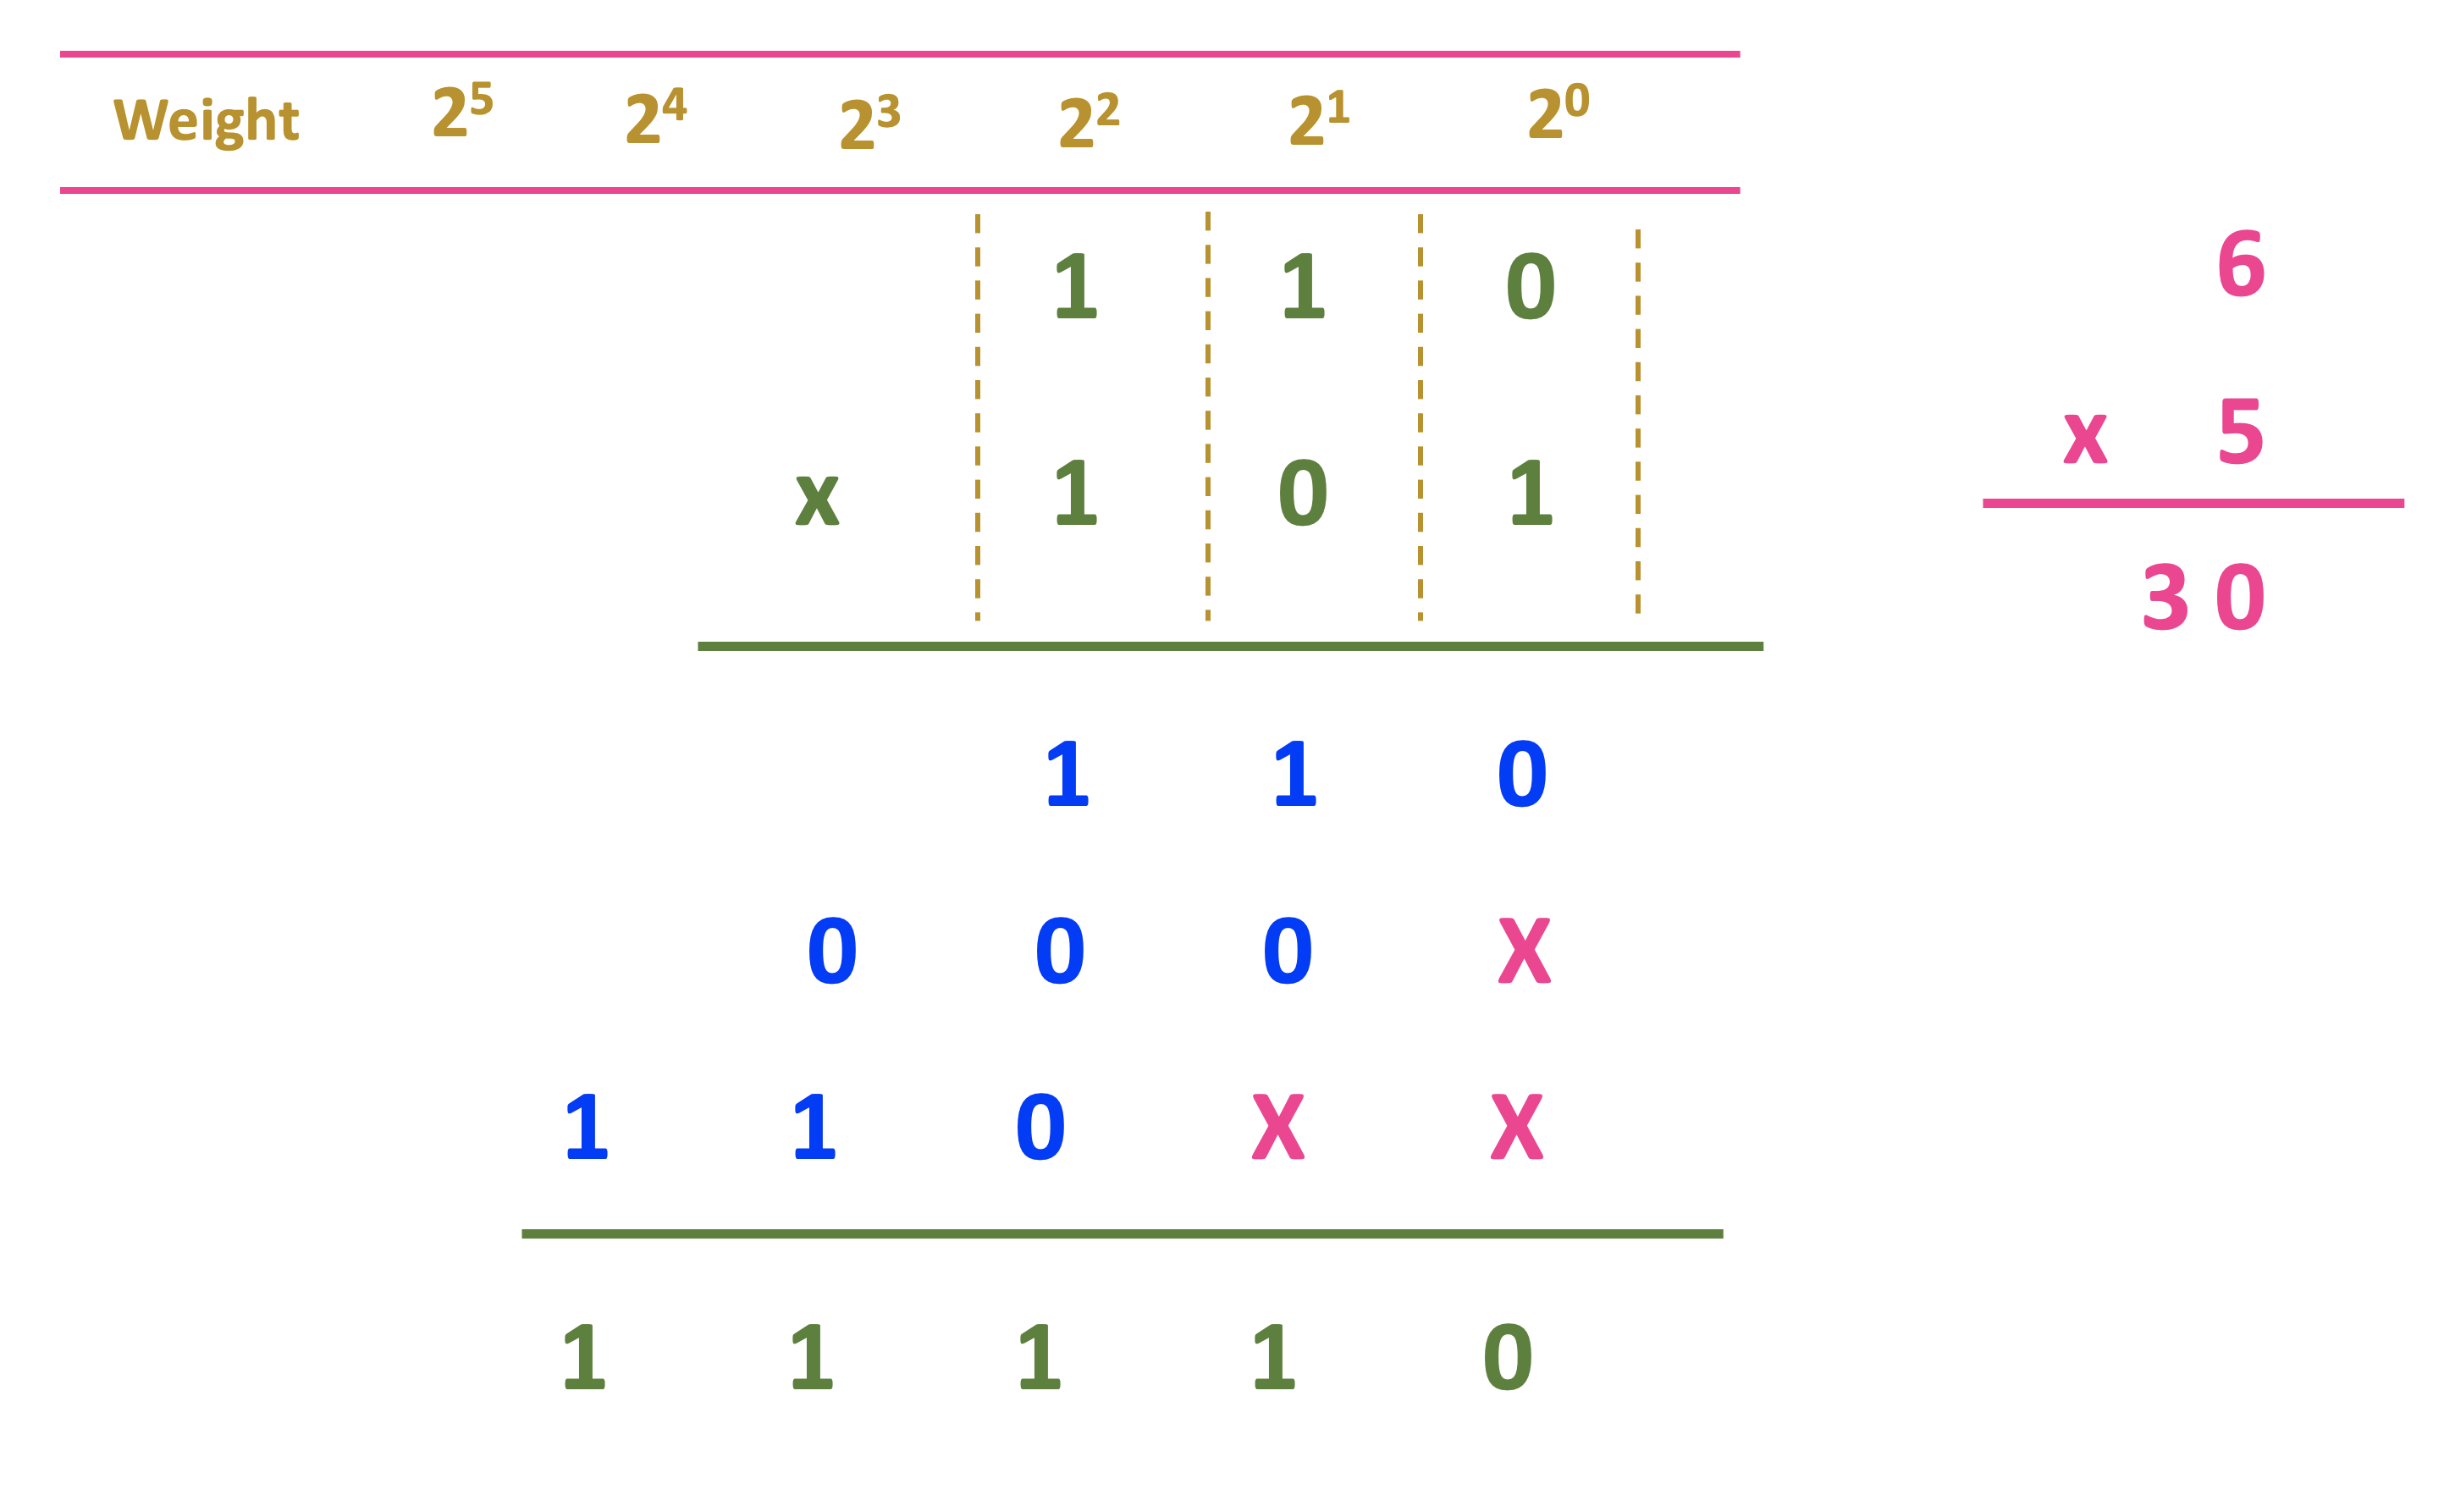
\includegraphics[width=0.8\textwidth]{figs/EM-Fig-unsigned_mul_PP.png}
    \caption{两个无符号整数的运算过程}
    \label{EM:Fig:unsigned_mul_PP_gen}
\end{figure}




\subsubsection{补码有符号乘法器}

无符号数不能表示负数,为了解决二进制下的问题,研究人员引入了原码(True form)、反码(1's complement)和补码(2's complement)来表示数据。
与无符号数相比,原码在最高位额外增加了一位符号位用来区分正负,0表示正数,1表示负数;在反码中,正数的反码就是其原码,负数的反码是将原码中,除符号位外,每一位按位取反;在补码中,正数的补码同样是其原码,负数的补码是其反码加一。
与原码和反码相比,补码避免了加减法不统一和存在两个零值的缺点,简化了硬件电路设计的复杂度,因此现代计算机底层采用补码的编码方式对数据进行存储和运算。
若式\eqref{EM:Eq:unsigned_fixed_Binary}为补码,$R=2$时,其最高位权重为$-2^{n-1}$,式\eqref{EM:Eq:unsigned_fixed_Decimal}变为:
% \begin{equation}
\begin{align}
    % V(A) = & \ D(A_2) \notag \\
    % = & \ ( \ \textcolor{red}{-}a_{n-1} \times R^{n-1} + a_{n-2} \times R^{n-2} + \cdots + a_1 \times R^1 + a_0 \times R^0 + \notag \\
    % & \ a_{-1} \times R^{-1} + a_{-2} \times R^{-2} + \cdots + a_{-m+1} \times R^{-m+1} + a_{-m} \times R^{-m} \ )_{10} \notag \\
    % = & \  ( \ \textcolor{red}{-}a_{n-1} \times 2^{n-1} + a_{n-2} \times 2^{n-2} + \cdots + a_1 \times 2^1 + a_0 \times 2^0 + \label{EM:Eq:signed_fixed_Decimal} \\
    % & \ a_{-1} \times 2^{-1} + a_{-2} \times 2^{-2} + \cdots + a_{-m+1} \times 2^{-m+1} + a_{-m} \times 2^{-m} \ )_{10} \notag \\
    % = & \ ( \textcolor{red}{-}a_{n-1} \times 2^{n-1} + \sum_{i=-m}^{n-2} a_i \times 2^i \ )_{10} \notag
    V(A) = & \ \textcolor{red}{-}a_{n-1}  R^{n-1} + a_{n-2}  R^{n-2} + \cdots + a_1  R^1 + a_0  R^0 + \notag \\
    & \ a_{-1}  R^{-1} + a_{-2}  R^{-2} + \cdots + a_{-m+1}  R^{-m+1} + a_{-m}  R^{-m} \notag \\
    = & \ \textcolor{red}{-}a_{n-1}  2^{n-1} + a_{n-2}  2^{n-2} + \cdots + a_1  2^1 + a_0  2^0 + \notag \\
    & \ a_{-1}  2^{-1} + a_{-2}  2^{-2} + \cdots + a_{-m+1}  2^{-m+1} + a_{-m}  2^{-m} \notag \\
    = & \ \textcolor{red}{-}a_{n-1}  2^{n-1} + \sum_{i=-m}^{n-2} a_i  2^i
\label{EM:Eq:signed_fixed_Decimal}
\end{align}
% \end{equation}

这里$n+m \ge 2$(引入了一位符号位),$n=1$和$m=0$时分别表示补码纯小数和补码整数。若不局限于二进制,式\eqref{EM:Eq:signed_fixed_Decimal}不一定成立%
\IfStrEq{\Version}{Open}{%
    \footnote{\url{https://blog.csdn.net/mydreamongo/article/details/8863502}},
}{,}
即任意$R$进制下,补码的最高位权重不一定是$-R^{n-1}$。
另外,一般地,对一个$N$位二进制定点数,忽略小数点,不同编码方式能够表示的数值范围为:
% \begin{equation}
% \begin{align}
%     & \text{无符号数:}  & [0, \ R^N-1] \ , \\
%     & \text{原码与反码:}  & [- \lfloor \frac{R^N-1}{2} \rfloor, \ \lfloor \frac{R^N-1}{2} \rfloor] \ , \\
%     & \text{补码:} & [- \lceil \frac{R^N-1}{2} \rceil, \ \lfloor \frac{R^N-1}{2} \rfloor] \ .
% \end{align}
% \end{equation}
\begin{align}
    & \text{无符号数:}  & [0, \ 2^N-1] \ , \\
    & \text{原码与反码:}  & [- \lfloor \frac{2^N-1}{2} \rfloor, \ \lfloor \frac{2^N-1}{2} \rfloor] \ , \\
    & \text{补码:} & [- \lceil \frac{2^N-1}{2} \rceil, \ \lfloor \frac{2^N-1}{2} \rfloor] \ .
\end{align}
式中$\lfloor \ \rfloor$和$\lceil \ \rceil$分别表示向下取整和向上取整。例如,$N=8$时,原码和反码的表示范围为[-127,127],补码的表示范围为[-128,127]。
% $R=3$,$N=4$时,原码、反码和补码的表示范围均为[-40,40]。
% \textcolor{red}{之后的内容,只要不特殊说明,均基于二进制($R=2$)。}

对于补码有符号二进制乘法器(Signed binary multiplier),目前常见的部分积生成方法有:符号位扩展、改进的Baugh–Wooley算法\cite{EM:baugh-wooley,EM:baugh-wooley_modified_PP_reorga,EM:baugh-wooley_diff}、以及基4的布斯编码\cite{EM:booth_orig,EM:booth_Macsorley,EM:booth_proof}。下面分别进行介绍:

(1)符号位扩展。

按照实现细节分类,符号位扩展方法分为两种:一种是操作数(Operand)符号位扩展,优点是硬件不需要支持减法,缺点是部分积的规模巨大,累加电路非常复杂;第二种是部分积符号位扩展,优点是不需要修改操作数,部分积的规模适中,缺点是需要对最后一个部分积执行减法。具体细节如下:
\begin{itemize}
    \item 操作数符号位扩展:首先根据乘数和被乘数确定乘积的位宽,然后将两个操作数的位宽扩展到乘积位宽,扩展方法为高位符号位扩展,即正数进行0扩展,负数进行1扩展;之后仿照无符号数二进制乘法通过逻辑与(AND)得到部分积;最后进行累加求和,注意求和后的结果应根据乘积的正确位宽进行截断。
    \item 部分积符号位扩展:同样先确定乘积所需要的位宽,不修改操作数,通过逻辑与(AND)得到部分积;然后对部分积进行高位符号位扩展(正数0扩展,负数1扩展),将每个部分积的位宽扩展到乘积位宽;最后对部分积进行累加,但对最后一个部分积执行减法。注意对于二进制补码来说, $-[A]_\text{补} = [-A]_\text{补}$,即可以通过“按位取反加1,符号位进位舍弃”的方法得到一个补码的相反数,将减法转换为加法。
\end{itemize}
% \begin{figure}[!htb]
%     \centering
%     \subfigure[操作数符号位扩展示意图。]{
%     \label{EM:Fig:操作数符号位扩展}
%     \begin{minipage}[t]{0.54\linewidth}
%     \centering
%     \includegraphics[width=\linewidth]{figs/EM:Fig:操作数符号位扩展.pdf}
%     \end{minipage}
%     }\ \ \ 
%     \subfigure[部分积符号位扩展示意图。]{
%     \label{EM:Fig:部分积符号位扩展}
%     \begin{minipage}[t]{0.4\linewidth}
%     \centering
%     \includegraphics[width=\linewidth]{figs/EM:Fig:部分积符号位扩展.pdf}
%     \end{minipage}
%     }
% \caption{补码乘法器的两种符号位扩展方法示意图}
% \label{EM:Fig:signed_mul_sign_extension}
% \end{figure}
\begin{figure}[!htb]
    \centering
    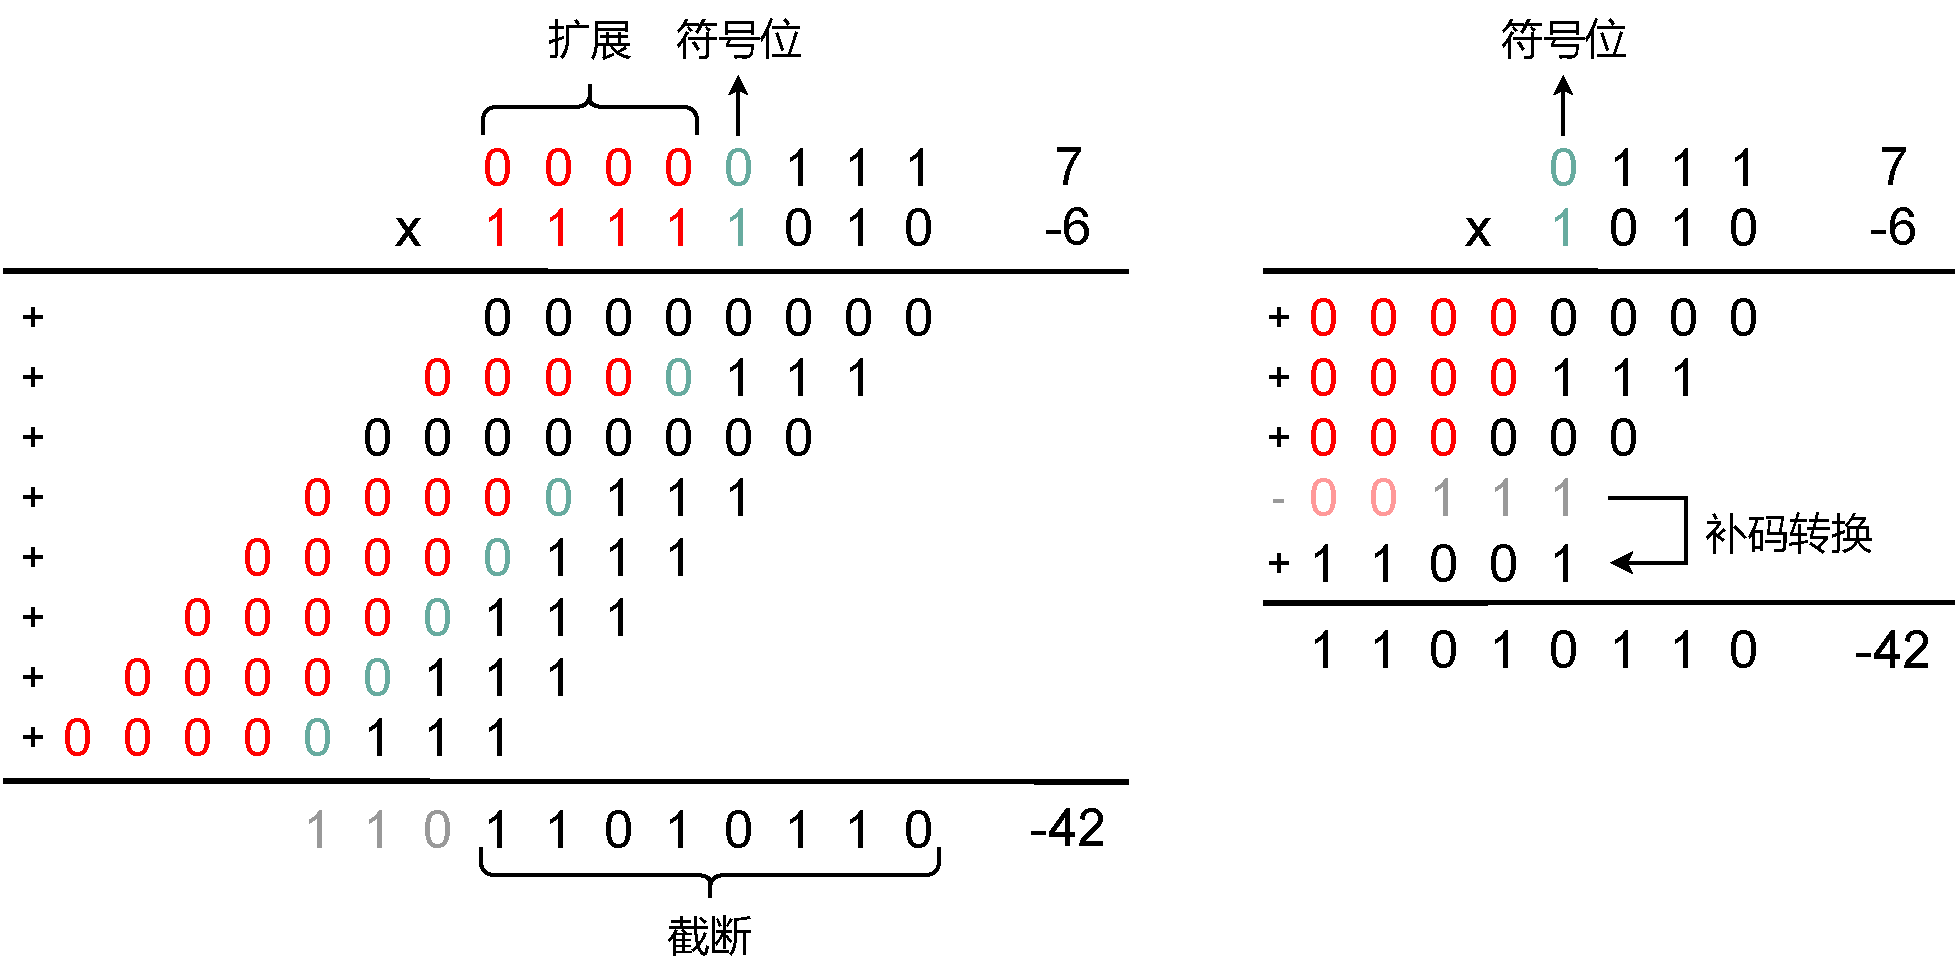
\includegraphics[width=\textwidth]{figs/EM-Fig-符号位扩展.pdf}
    \caption{补码乘法器的符号位扩展示例:左:操作数符号位扩展,右:部分积符号位扩展。}
    \label{EM:Fig:signed_mul_sign_extension}
\end{figure}

图\ref{EM:Fig:signed_mul_sign_extension}举例说明了两种符号位扩展方法的不同之处。可以看到,与操作数扩展相比,部分积扩展需要的加法更少,对应的硬件实现也更具有优势。然而,与无符号乘法相比,符号位扩展总会增大部分积的规模,使电路设计更复杂。有没有办法能够将其降低到和无符号乘法同一个水平?改进的Baugh-Wooley算法是一种解决方案\cite{EM:baugh-wooley,EM:baugh-wooley_modified_PP_reorga,EM:baugh-wooley_diff}。

(2)改进的Baugh-Wooley算法 \label{改进的Baugh-Wooley算法}

Baugh-Wooley算法是由Baugh和Wooley于1973年提出的用于二进制补码相乘的算法\cite{EM:baugh-wooley},该算法对权重为负的部分积进行修正,避免了符号位扩展,原理如下:

\noindent 设$m=0$,由式\eqref{EM:Eq:signed_fixed_Decimal}得两个$n$比特整数$X = x_{n-1} x_{n-2} \cdots x_1 x_0$和$Y = y_{n-1} y_{n-2} \cdots y_1 y_0$的十进制值:
\begin{equation}
    V(X) = -x_{n-1} 2^{n-1} + \sum_{i=0}^{n-2} x_i 2^i \ \ \ \ \ \ \ \
    V(Y) = -y_{n-1} 2^{n-1} + \sum_{i=0}^{n-2} y_i 2^i
\label{EM:Eq:signed_comp_XY}
\end{equation}
其乘积$P$:
% \begin{equation}
\begin{align}
    V(P) = & \ V(X)V(Y) \notag \\
    = & \ ( \textcolor{red}{-x_{n-1}  2^{n-1}} + \textcolor{magenta}{\sum_{i=0}^{n-2} x_i  2^i} ) \times
    ( \textcolor{blue}{-y_{n-1}  2^{n-1}} + \textcolor{cyan}{\sum_{i=0}^{n-2} y_i  2^i} ) \notag \\
%
    = & \ \textcolor{red}{x_{n-1}} \textcolor{blue}{y_{n-1}}  2^{2n-2} +
    \textcolor{magenta}{\sum_{i=0}^{n-2} x_i 2^i} \textcolor{cyan}{\sum_{j=0}^{n-2} y_j 2^j}
    \textcolor{red}{-x_{n-1}  2^{n-1}} \textcolor{cyan}{\sum_{i=0}^{n-2} y_i  2^i}
    \textcolor{blue}{-y_{n-1}  2^{n-1}} \textcolor{magenta}{\sum_{i=0}^{n-2} x_i  2^i} \notag \\
%
    = & \ \textcolor{red}{x_{n-1}} \textcolor{blue}{y_{n-1}}  2^{2n-2} +
    \textcolor{magenta}{\sum_{i=0}^{n-2}} \textcolor{cyan}{\sum_{j=0}^{n-2}} \textcolor{magenta}{x_i} \textcolor{cyan}{y_j} 2^{\textcolor{magenta}{i}+\textcolor{cyan}{j}} 
    \textcolor{red}{-2^{n-1}} \textcolor{cyan}{\sum_{i=0}^{n-2}} \textcolor{red}{x_{n-1}} \textcolor{cyan}{y_i 2^i}
    \textcolor{blue}{-2^{n-1}} \textcolor{magenta}{\sum_{i=0}^{n-2}} \textcolor{blue}{y_{n-1}} \textcolor{magenta}{x_i 2^i}
\label{EM:Eq:signed_comp_P}
\end{align}
% \end{equation}
$n=5$时,式\eqref{EM:Eq:signed_comp_P}对应的部分积阵列如图\ref{EM:Fig:signed_mul_PP_array}所示,其中红色部分积的权重为负数,对应式\eqref{EM:Eq:signed_comp_P}中结果的后两项:
\begin{figure}[!htb]
    \centering
    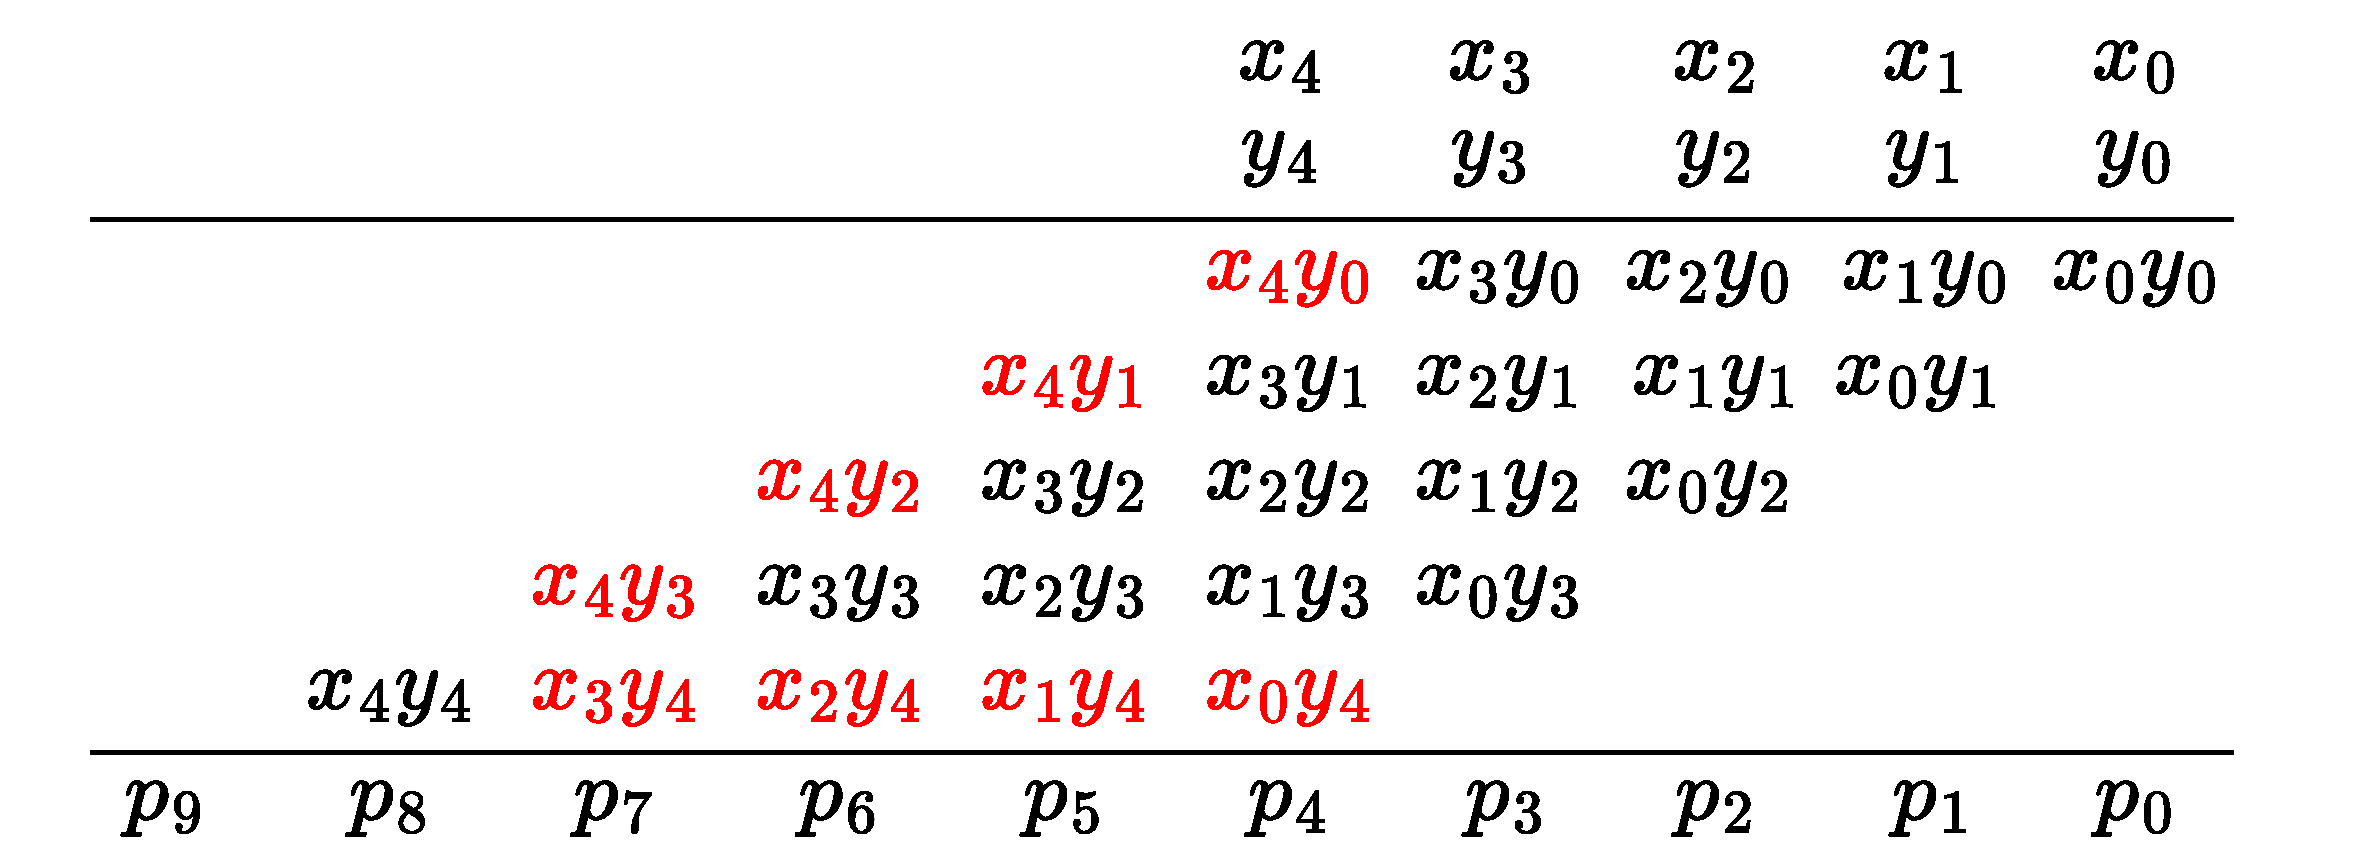
\includegraphics[width=0.85\textwidth]{figs/EM-Fig-补码部分积阵列.pdf}
    \caption{$5 \times 5$补码乘法器的部分积阵列示意图,红色部分积的权重为负}
    \label{EM:Fig:signed_mul_PP_array}
\end{figure}

\noindent 对于任意补码(不失一般性,假设是式\eqref{EM:Eq:signed_comp_XY}中的$X$):
\begin{equation}
    -V(X) = - \overline {x_{n-1}} 2^{n-1} + \sum_{i=0}^{n-2} \overline{x_i} 2^i +1 \ \ \text{(按位取反加1,符号位进位丢弃)}
    \label{EM:Eq:signed_comp_subtract}
\end{equation}
则式\eqref{EM:Eq:signed_comp_P}中结果的后两项变为:
% \begin{equation}
\begin{align}
& \textcolor{red}{-2^{n-1}} ( -0 \cdot 2^n + 0 \cdot 2^{n-1} + \textcolor{cyan}{\sum_{i=0}^{n-2}} \textcolor{red}{x_{n-1}} \textcolor{cyan}{y_i 2^i} )
\textcolor{blue}{-2^{n-1}} ( -0 \cdot 2^n + 0 \cdot 2^{n-1} + \textcolor{magenta}{\sum_{i=0}^{n-2}} \textcolor{blue}{y_{n-1}} \textcolor{magenta}{x_i 2^i} ) \notag \\
%
= & \textcolor{red}{+2^{n-1}} ( -1 \cdot 2^n + 1 \cdot 2^{n-1} + \textcolor{cyan}{\sum_{i=0}^{n-2}} \overline{ \textcolor{red}{x_{n-1}}  \textcolor{cyan}{y_i}}  \textcolor{cyan}{2^i} + 1 ) \
\textcolor{blue}{+2^{n-1}} ( -1 \cdot 2^n + 1 \cdot 2^{n-1} + \textcolor{magenta}{\sum_{i=0}^{n-2}} \overline{ \textcolor{blue}{y_{n-1}}  \textcolor{magenta}{x_i} } \textcolor{magenta}{2^i} + 1 ) \label{EM:Eq:signed_comp_P_Baugh-Wooley_positve}
\end{align}

\noindent 为了避免出现与非门(NAND),注意到式\eqref{EM:Eq:signed_comp_P_Baugh-Wooley_positve}中结果的第一项为:
\begin{equation}
    \left\{
    \begin{aligned}
        \ & 0 , & \ \ x_{n-1} = 0, \\
        \ & \textcolor{red}{+2^{n-1}} ( - 2^n + 2^{n-1} + \textcolor{cyan}{\sum_{i=0}^{n-2}} \overline{ \textcolor{cyan}{y_i}}  \textcolor{cyan}{2^i} + 1 ), & \ \ x_{n-1} = 1.
    \end{aligned}
    \right.
\end{equation}
即:
\begin{equation}
    \textcolor{red}{+2^{n-1}} ( - 2^n + 2^{n-1} + \overline{x_{n-1}} 2^{n-1} + x_{n-1} + \textcolor{cyan}{\sum_{i=0}^{n-2}} x_{n-1} \overline{ \textcolor{cyan}{y_i}}  \textcolor{cyan}{2^i} )
\label{EM:Eq:signed_comp_P_Baugh-Wooley_rNAND_x}
\end{equation}
同理第二项为:
\begin{equation}
    \left\{
    \begin{aligned}
        \ & 0 , & \ \ y_{n-1} = 0, \\
        \ & \textcolor{blue}{+2^{n-1}} ( - 2^n + 2^{n-1} + \textcolor{magenta}{\sum_{i=0}^{n-2}} \overline{ \textcolor{magenta}{x_i} } \textcolor{magenta}{2^i} + 1 ), & \ \ y_{n-1} = 1.
    \end{aligned}
    \right.
\end{equation}
即:
\begin{equation}
    \textcolor{blue}{+2^{n-1}} ( - 2^n + 2^{n-1} + \overline{y_{n-1}} 2^{n-1} + y_{n-1} + \textcolor{magenta}{\sum_{i=0}^{n-2}} y_{n-1} \overline{ \textcolor{magenta}{x_i} } \textcolor{magenta}{2^i} )
\label{EM:Eq:signed_comp_P_Baugh-Wooley_rNAND_y}
\end{equation}
结合式\eqref{EM:Eq:signed_comp_P}、式\eqref{EM:Eq:signed_comp_P_Baugh-Wooley_positve}、式\eqref{EM:Eq:signed_comp_P_Baugh-Wooley_rNAND_x}和式\eqref{EM:Eq:signed_comp_P_Baugh-Wooley_rNAND_y},$V(P)$变为:
\begin{equation}
\begin{aligned}
    V(P) = & \ \textcolor{red}{x_{n-1}} \textcolor{blue}{y_{n-1}}  2^{2n-2} +
    \textcolor{magenta}{\sum_{i=0}^{n-2}} \textcolor{cyan}{\sum_{j=0}^{n-2}} \textcolor{magenta}{x_i} \textcolor{cyan}{y_j} 2^{\textcolor{magenta}{i}+\textcolor{cyan}{j}} \\
%
    & \ \textcolor{red}{+2^{n-1}} ( - 2^n + 2^{n-1} + \overline{x_{n-1}} 2^{n-1} + x_{n-1} + \textcolor{cyan}{\sum_{i=0}^{n-2}} x_{n-1} \overline{ \textcolor{cyan}{y_i}}  \textcolor{cyan}{2^i} ) \\
%
    & \ \textcolor{blue}{+2^{n-1}} ( - 2^n + 2^{n-1} + \overline{y_{n-1}} 2^{n-1} + y_{n-1} + \textcolor{magenta}{\sum_{i=0}^{n-2}} y_{n-1} \overline{ \textcolor{magenta}{x_i} } \textcolor{magenta}{2^i} )
\end{aligned}
\label{EM:Eq:signed_comp_P_Baugh-Wooley}
\end{equation}
式\eqref{EM:Eq:signed_comp_P_Baugh-Wooley}被称为Baugh-Wooley算法,$n=5$时,该算法对应的部分积阵列如图\ref{EM:Fig:orig_Baugh-Wooley_PP}所示,所有比特权重均为正值(除了最高位的1)。与同位宽的无符号乘法器相比,不论$n$多大,由式\eqref{EM:Eq:signed_comp_P_Baugh-Wooley}得到的部分积阵列只会增加5个比特,大大优于符号位扩展方法。然而,原始的Baugh-Wooley方法会导致部分积阵列增加两层(如图\ref{EM:Fig:orig_Baugh-Wooley_PP}中的$x_4$与$y_4$),不利于后续的累加操作,注意到式\eqref{EM:Eq:signed_comp_P_Baugh-Wooley_positve}可变为:
\begin{equation}
\textcolor{red}{+2^{n-1}}  \textcolor{cyan}{\sum_{i=0}^{n-2}} \overline{ \textcolor{red}{x_{n-1}}  \textcolor{cyan}{y_i}}  \textcolor{cyan}{2^i}
\textcolor{blue}{+2^{n-1}} \textcolor{magenta}{\sum_{i=0}^{n-2}} \overline{ \textcolor{blue}{y_{n-1}}  \textcolor{magenta}{x_i} } \textcolor{magenta}{2^i} + 1 \cdot 2^n -1 \cdot 2^{2n-1}
\label{EM:Eq:signed_comp_P_Baugh-Wooley_modified}
\end{equation}
Hatamian等人根据式\eqref{EM:Eq:signed_comp_P_Baugh-Wooley_modified}对部分积进行了重新排列\cite{EM:baugh-wooley_modified_PP_reorga},得到了\ref{EM:Fig:modified_Baugh-Wooley_PP},被称为改进的Baugh-Wooley算法%
\IfStrEq{\Version}{Open}{%
    \footnote{\url{https://zhuanlan.zhihu.com/p/343133392}},
}{,}
只对部分积引入两个1,不增加部分积阵列的层数,得到了广泛的应用\cite{EM:baugh-wooley_diff}。

\begin{figure}[!htb]
    \centering
    \subfigure[原始的Baugh-Wooley乘法器部分积阵列]{
    \label{EM:Fig:orig_Baugh-Wooley_PP}
    \begin{minipage}[t]{0.48\linewidth}
    \centering
    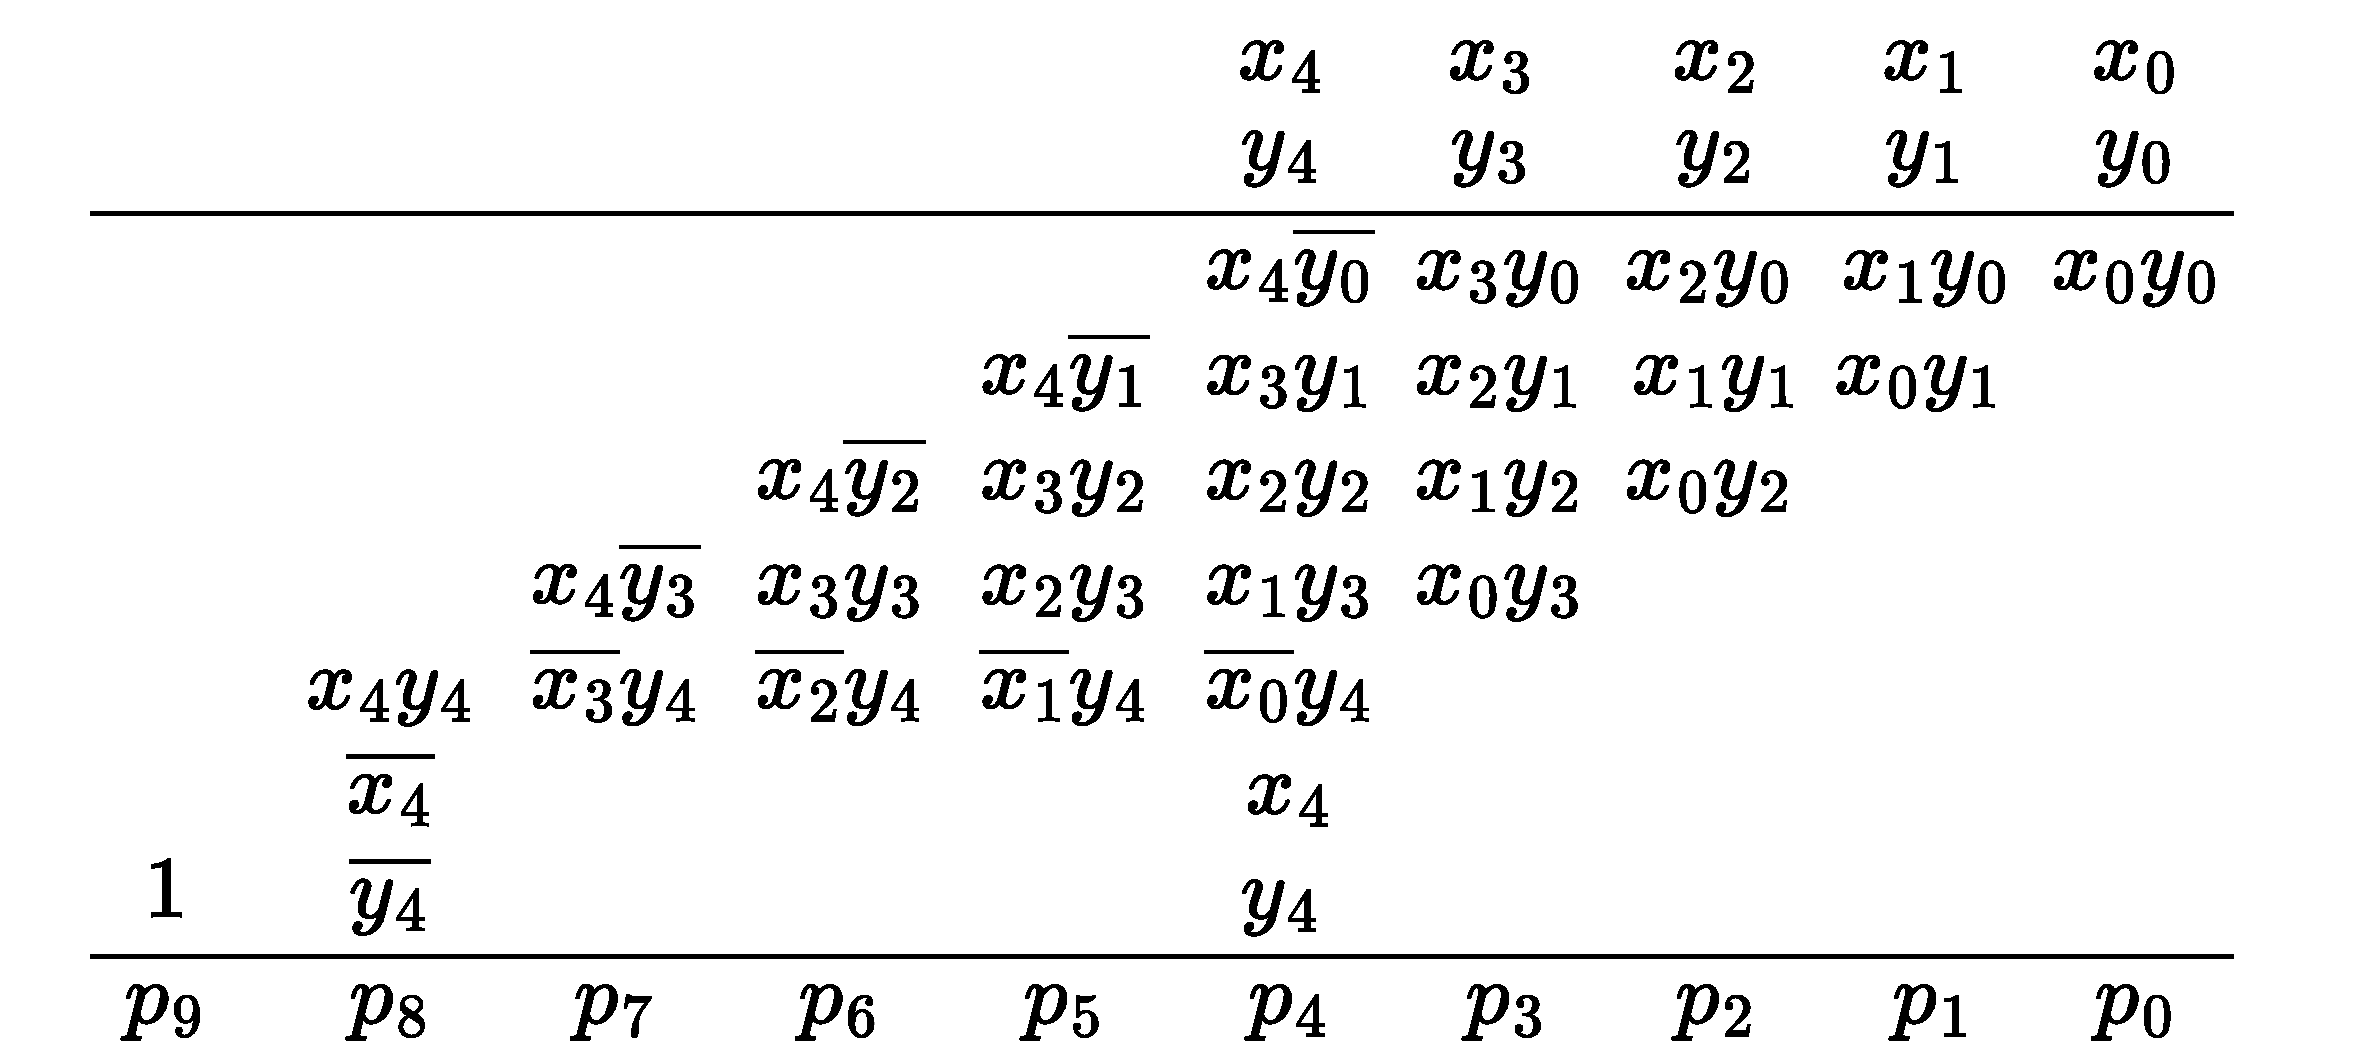
\includegraphics[width=\linewidth]{figs/EM-Fig-Baugh-Wooley.pdf}
    \end{minipage}
    }
    \subfigure[改进的Baugh-Wooley乘法器部分积阵列]{
    \label{EM:Fig:modified_Baugh-Wooley_PP}
    \begin{minipage}[t]{0.48\linewidth}
    \centering
    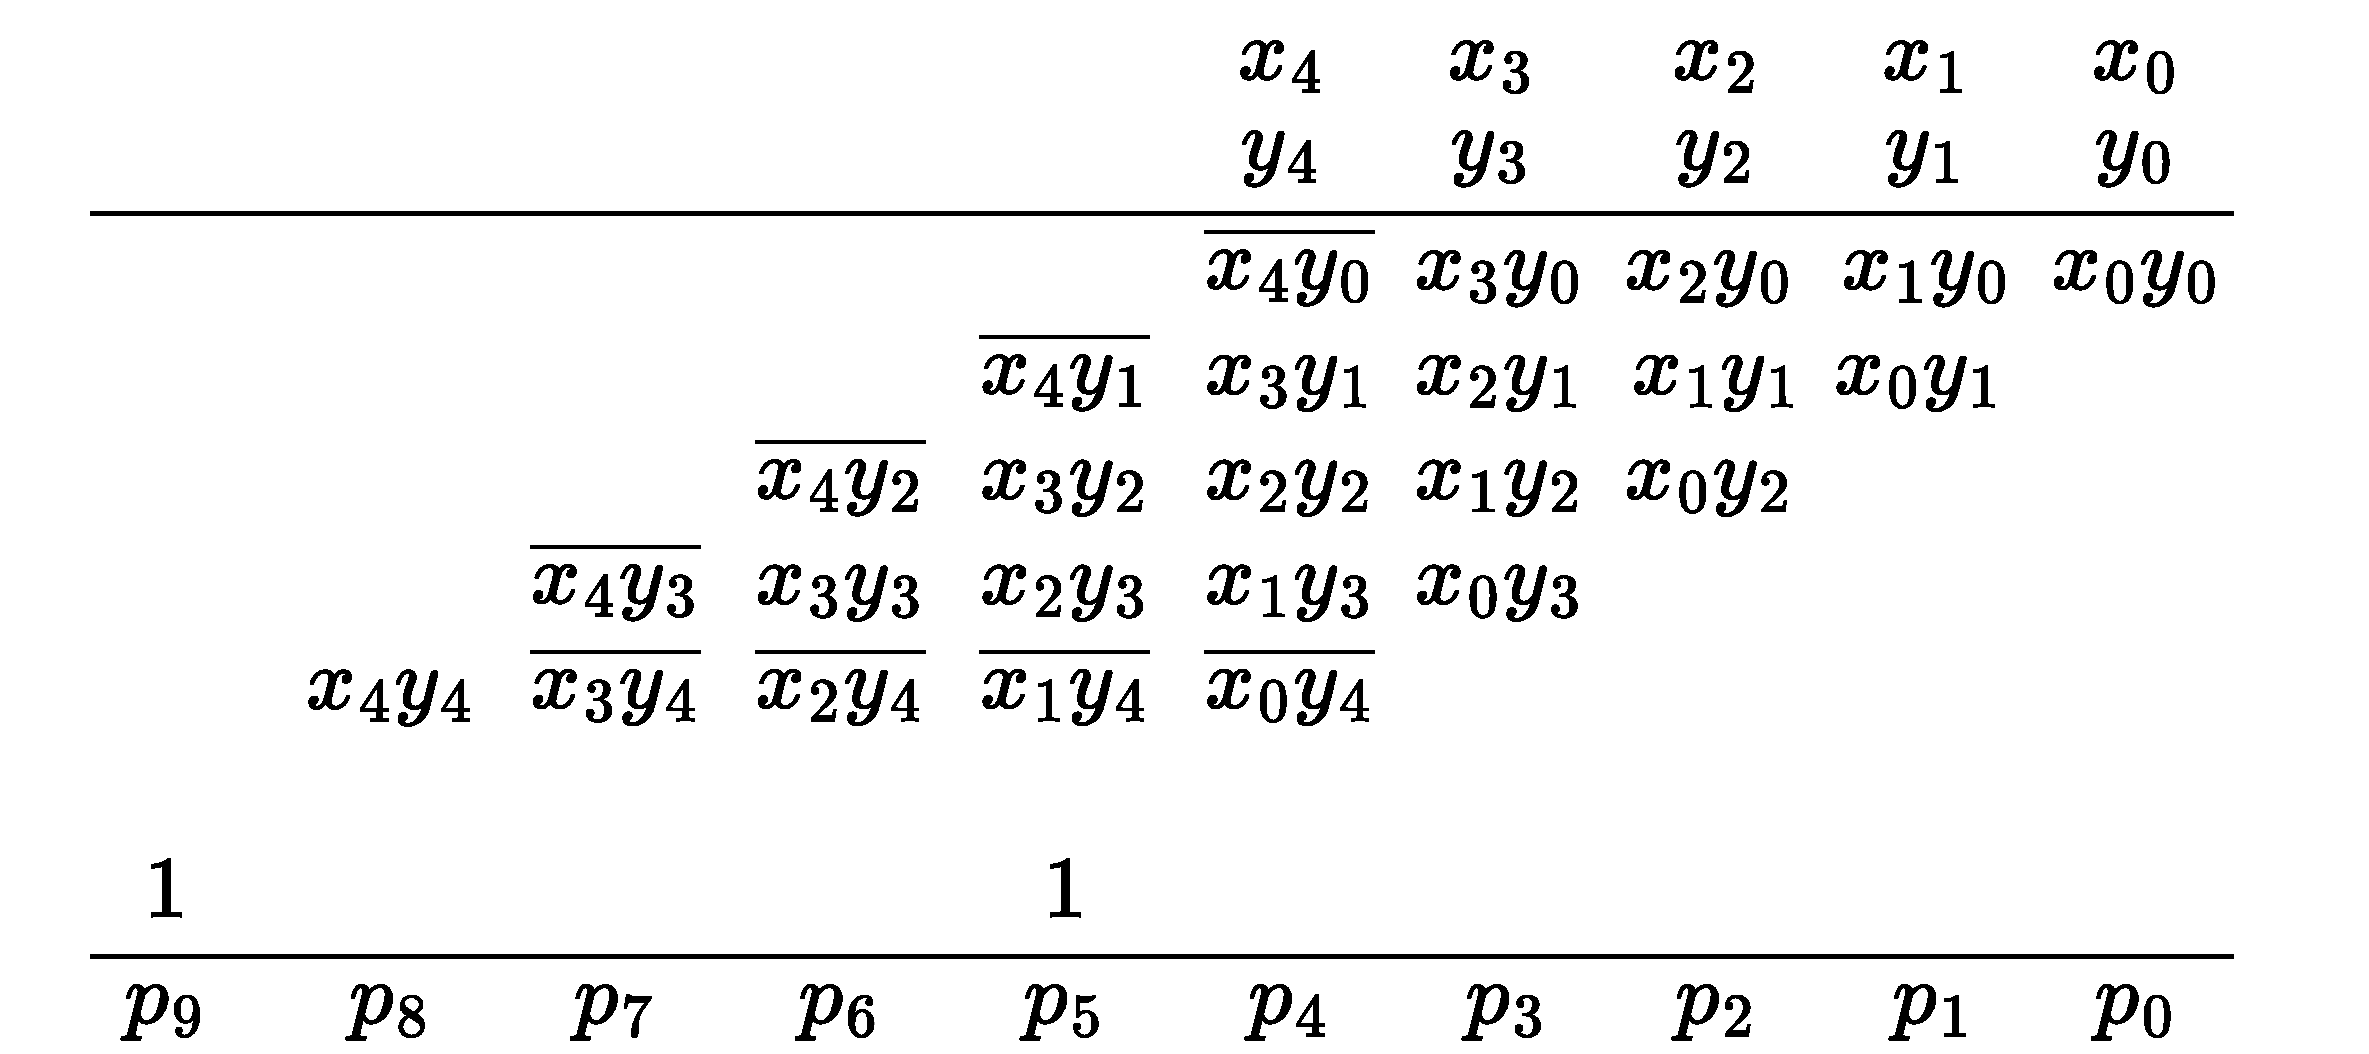
\includegraphics[width=\linewidth]{figs/EM-Fig-改进的Baugh-Wooley.pdf}
    \end{minipage}
    }
\caption{基于Baugh-Wooley算法设计的$5 \times 5$补码乘法器的部分积阵列示意图}
\label{EM:Fig:signed_comp_P_Baugh-Wooley}
\end{figure}

(3)基4的布斯编码

与Baugh-Wooley算法不同,布斯编码的意义在于能够减少乘法器中部分积的个数(行数),且基数越高效果越明显,比如基4和基8的布斯编码分别能够将部分积的个数降低一半和三分之二\cite{EM:booth_Macsorley,EM:booth_proof},大大减轻后续的累加压力。然而,高基的布斯编码电路实现复杂,目前最常用的基数是4,原理如下:

对于补码有符号乘法,假设$n$为偶数,$y_{-1} = 0$,式\eqref{EM:Eq:signed_comp_XY}中的$V(Y)$变为:
\begin{align}
    V(Y) = & \ - y_{n-1} 2^{n-1} + y_{n-2} 2^{n-2} + y_{n-3} 2^{n-3} + y_{n-4} 2^{n-4} + y_{n-5} 2^{n-5} + \cdots + \notag \\
%
    & y_5 2^5 + y_4 2^4 + y_3 2^3 + y_2 2^2 + y_1 2^1 + y_0 2^0 + \textcolor{red}{y_{-1} 2^{-1}} \notag \\
%
    = & \ ( -2 y_{n-1} + y_{n-2} + y_{n-3}) 2^{n-2} + (-2 y_{n-3} + y_{n-4} + y_{n-5}) 2^{n-4} + \cdots + \notag \\
%
    & \ (-2 y_5 + y_4 + y_3) 2^4 + (-2 y_3 + y_2 + y_1) 2^2 + (-2 y_1 + y_0 + \textcolor{red}{y_{-1}} ) 2^0
\label{EM:Eq:Radix-4-booth_VY}
\end{align}
式\eqref{EM:Eq:signed_comp_P}变为:
\begin{align}
    V(P) = & \ V(X)V(Y) \notag \\
    = & \ V(X) ( -2 y_{n-1} + y_{n-2} + y_{n-3}) 2^{n-2} + \notag \\
%
    & \ V(X) (-2 y_{n-3} + y_{n-4} + y_{n-5}) 2^{n-4} + \cdots + \notag \\
%
    & \ V(X) (-2 y_5 + y_4 + y_3) 2^4 + \notag \\
    & \ V(X) (-2 y_3 + y_2 + y_1) 2^2 + \notag \\
    & \ V(X) (-2 y_1 + y_0 + \textcolor{red}{y_{-1}} ) 2^0
    \label{EM:Eq:Radix-4-booth}
\end{align}
即是基4的布斯编码算法公式,其中$X$是被乘数,$Y$是乘数,对应的编码规则及部分积操作如表\ref{EM:Tab:Radix-4-booth}所示。该算法在进行前需要在乘数的最右侧隐含地补一个0,之后从最低有效位开始每次扫描3位乘数生成部分积,共$\dfrac{n}{2}$个,然后对部分积进行符号位扩展、累加并最终相加。由表\ref{EM:Tab:Radix-4-booth}可以看出,基4的布斯算法只涉及加法、减法和移位操作,硬件实现友好。
需要注意的是,式\eqref{EM:Eq:Radix-4-booth}仅适用于$n$是偶数的情况,若$n$是奇数,需先对乘数进行一位符号位扩展,将位宽变为偶数,之后再进行编码,此时部分积总数变为$\dfrac{n+1}{2}$个。布斯编码得到的部分积仍然需要符号位扩展,扩展后的累加电路复杂,可考虑采用改进的符号位扩展方法对其进行优化。

\begin{table}
\centering
\caption{基4布斯编码表}
\begin{tabular}{|c|c|c|c|c|} \hline
$y_{i+1}$ & $y_i$ & $y_{i-1}$ & $-2 y_{i+1} + y_i + y_{i-1}$ & \text{部分积操作} \\ \hline
0 & 0 & 0 & 0 & +0 \\ \hline
0 & 0 & 1 & 1 & $+[X]_{\text{补}}$ \\ \hline
0 & 1 & 0 & 1 & $+[X]_{\text{补}}$ \\ \hline
0 & 1 & 1 & 2 & $+2[X]_{\text{补}}$ \\ \hline
1 & 0 & 0 & -2 & $-2[X]_{\text{补}}$ \\ \hline
1 & 0 & 1 & -1 & $-[X]_{\text{补}}$ \\ \hline
1 & 1 & 0 & -1 & $-[X]_{\text{补}}$ \\ \hline
1 & 1 & 1 & 0 & +0 \\ \hline
\end{tabular}
\label{EM:Tab:Radix-4-booth}
\end{table}

除了补码有符号数乘法,布斯算法也可以用于无符号数相乘%
\IfStrEq{\Version}{Open}{%
    \footnote{\url{https://picture.iczhiku.com/resource/eetop/whKDFaTwqTZOkCxn.pdf}},
}{,}
为了支持布斯编码中需要的减法操作,无符号乘法的部分积也应采用补码格式。若基数取4,编码形式仍然是$-2 y_{i+1} + y_i + y_{i-1}$,但与补码乘法的区别在于:(a)$n$是偶数时需要添加的不仅是$y_{-1} = 0$,还有$y_{n+1} = y_n = 0$,此时$\{y_{n+1}, y_n, y_{n-1} \}$编码得到的部分积一定是0或正数,部分积总数为$\dfrac{n}{2} + 1$个;(b)$n$是奇数时需要添加$y_n = y_{-1} = 0$,部分积总数为$\dfrac{n+1}{2}$个;(c)改进的符号位扩展方法实现细节略有不同。

下面具体讲解基4布斯算法在无符号数乘法和补码有符号数乘法中,如何对部分积符号位扩展方法进行改进\cite{EM:booth_sign_extension}:


\begin{figure}[!htb]
    \centering
    \subfigure[部分积均为正数,省略了高位的0扩展]{
    \label{EM:Fig:booth_16x16_unsign_PP_positive}
    \begin{minipage}[t]{0.48\linewidth}
    \centering
    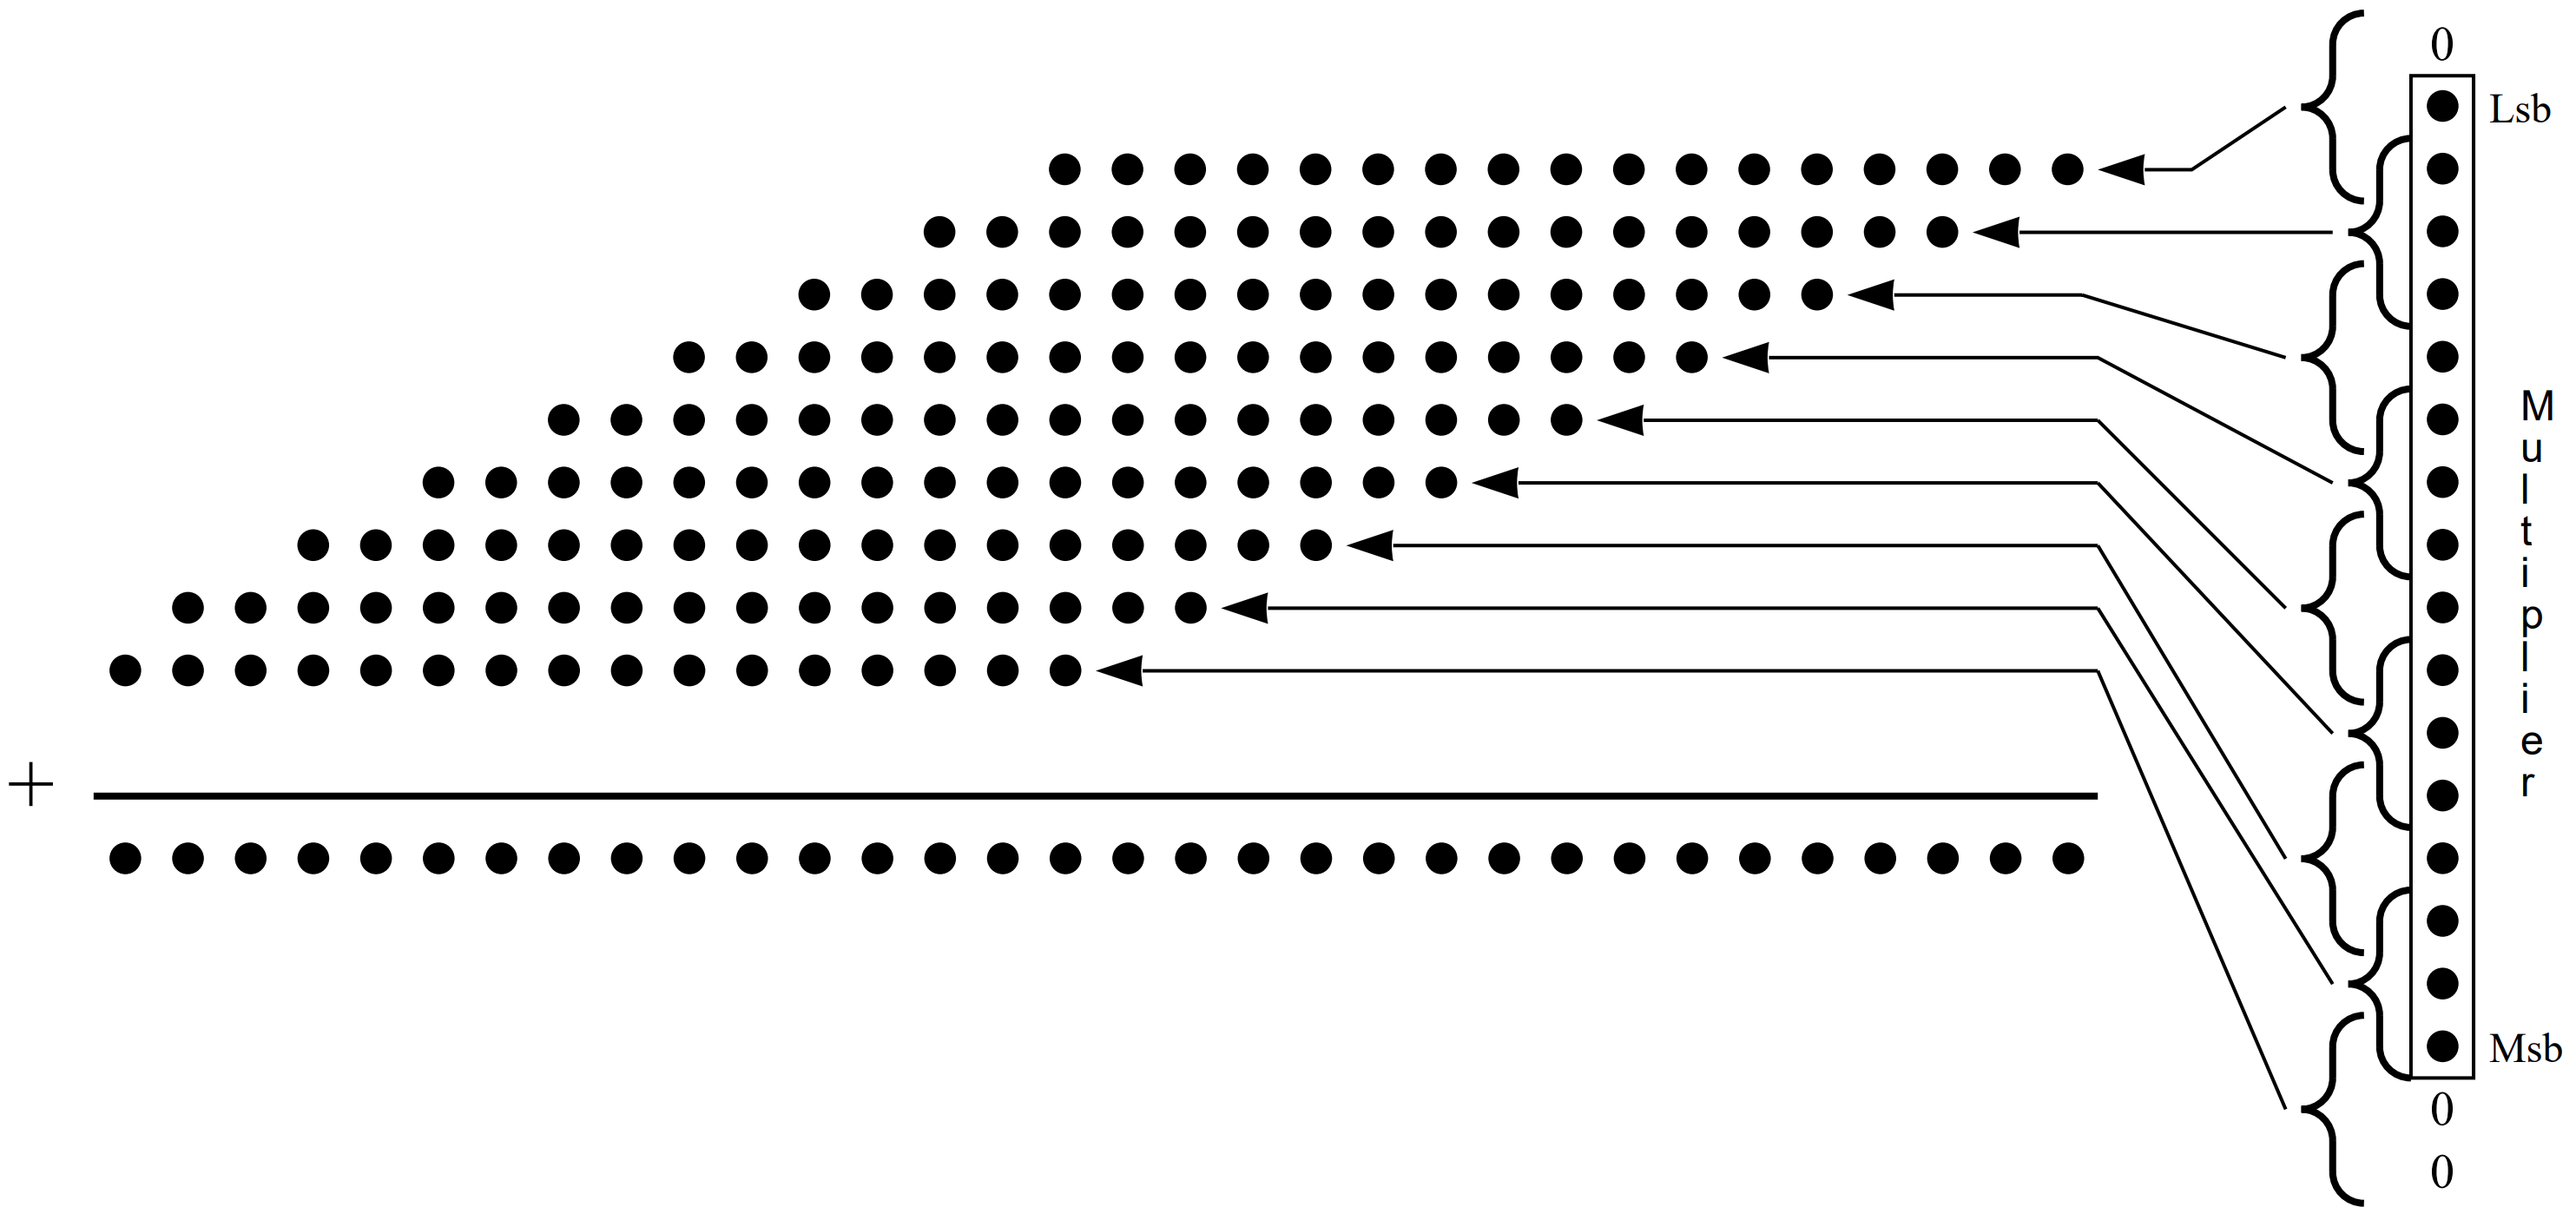
\includegraphics[width=\linewidth]{figs/EM-Fig-booth_unsign_positive.png}
    \end{minipage}
    }
    \subfigure[部分积均为负数,高位进行1扩展]{
    \label{EM:Fig:booth_16x16_unsign_PP_negtive}
    \begin{minipage}[t]{0.48\linewidth}
    \centering
    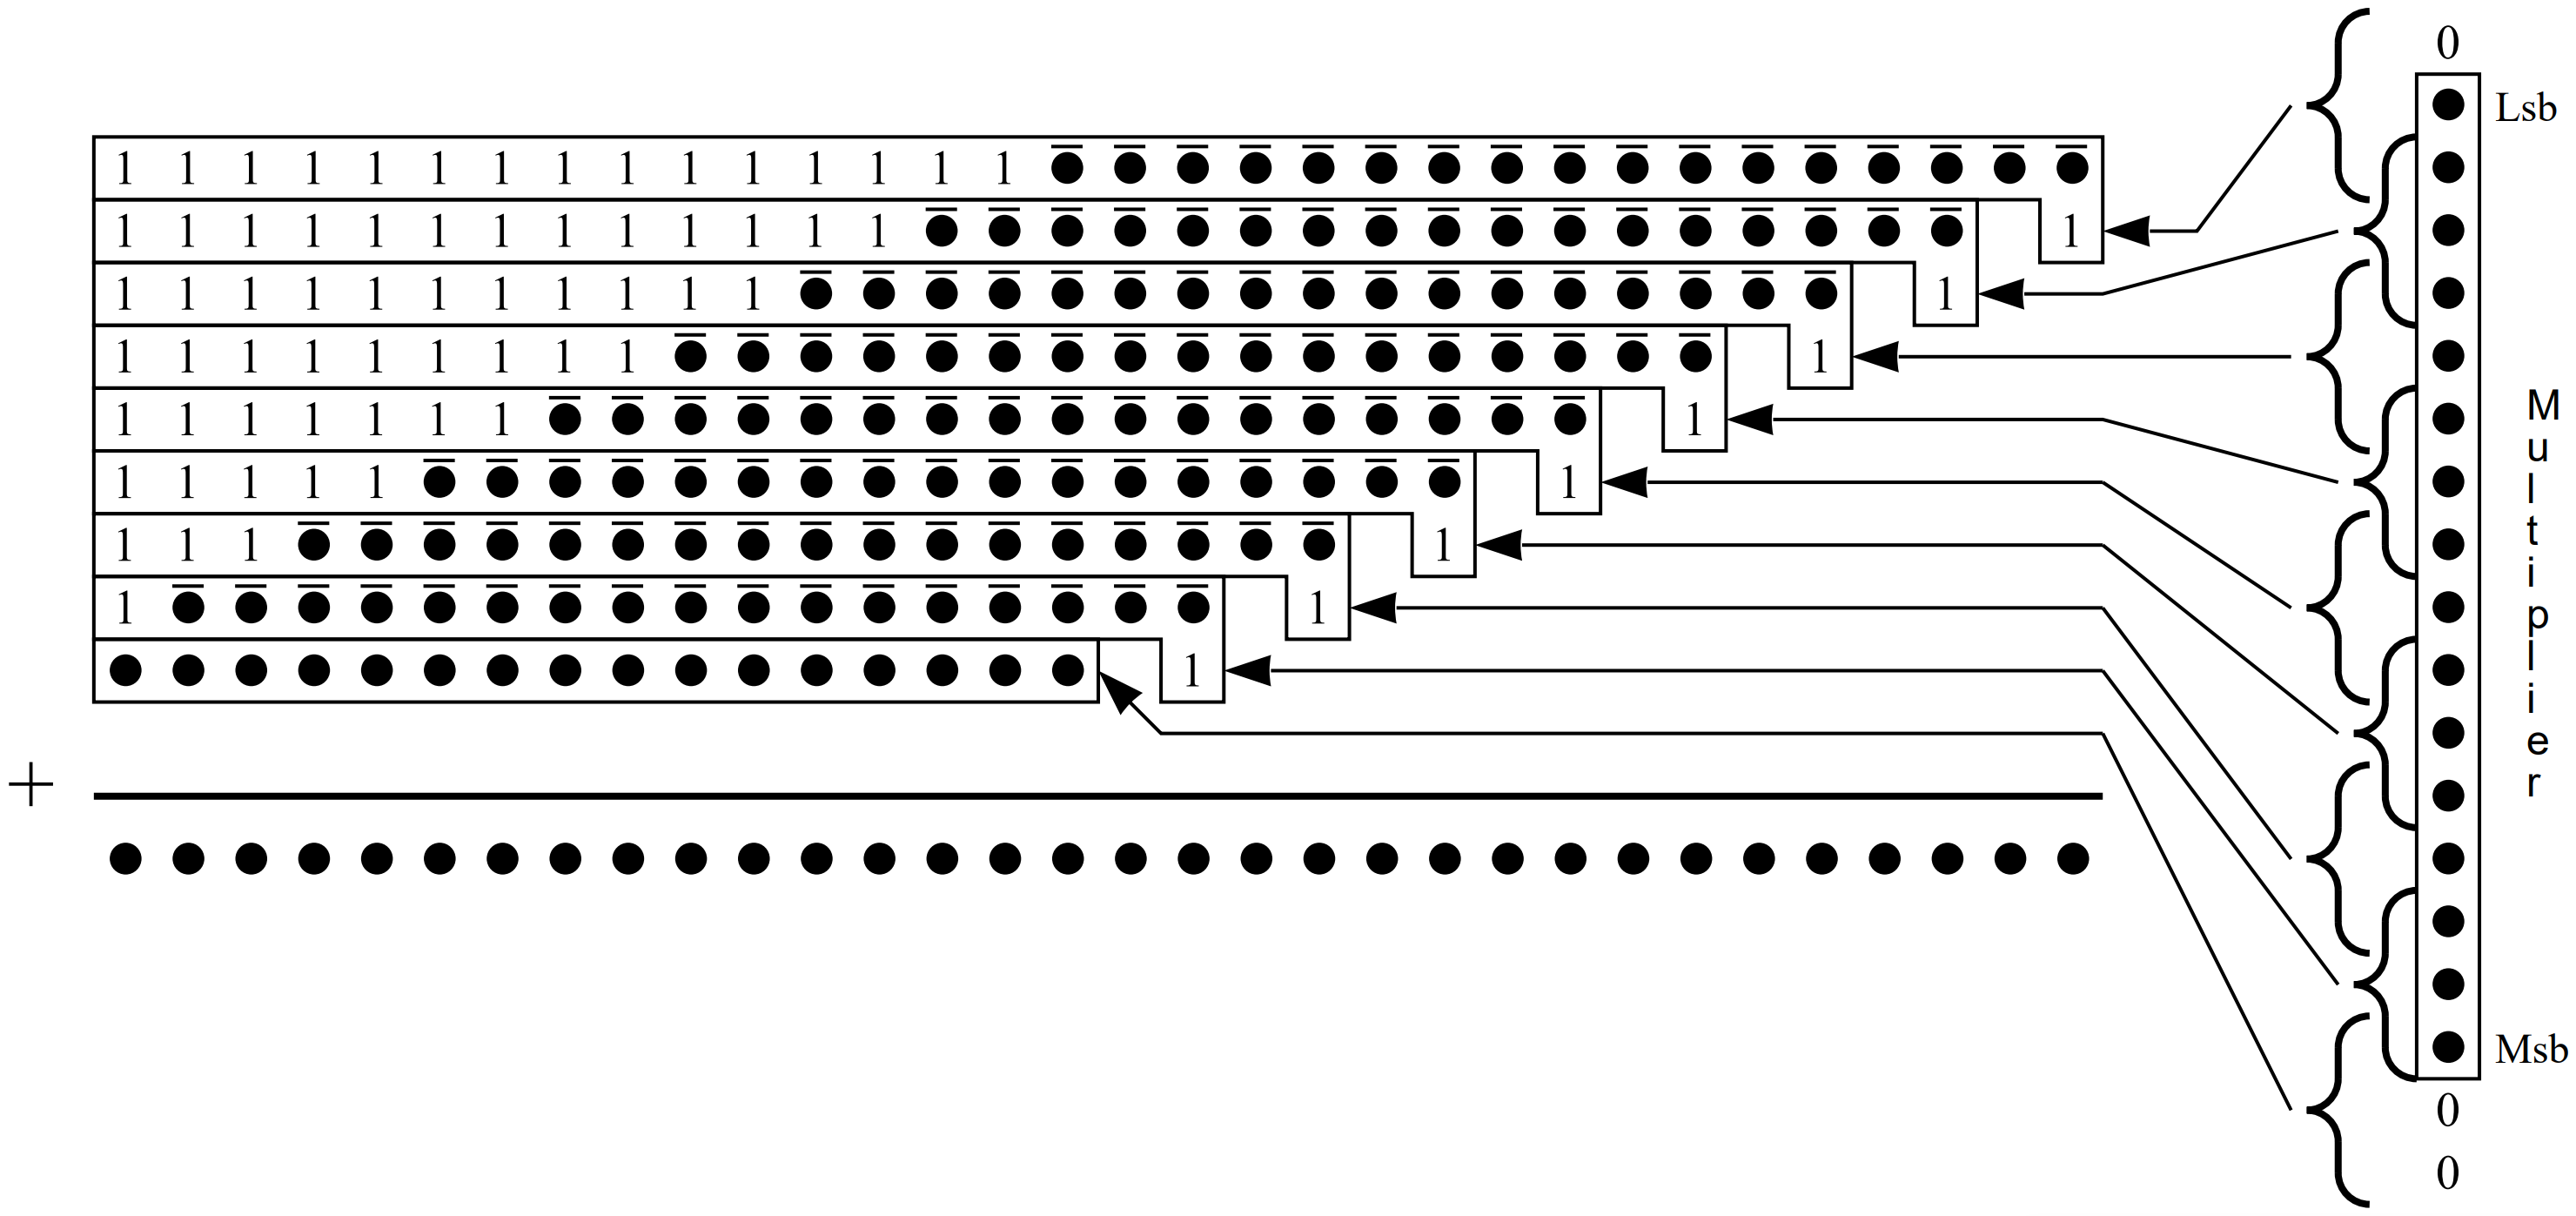
\includegraphics[width=\linewidth]{figs/EM-Fig-booth_unsign_negtive.png}
    \end{minipage}
    }
    \subfigure[部分积均为负数,高位进行1扩展后累加]{
    \label{EM:Fig:booth_16x16_unsign_PP_negtive_summed}
    \begin{minipage}[t]{0.48\linewidth}
    \centering
    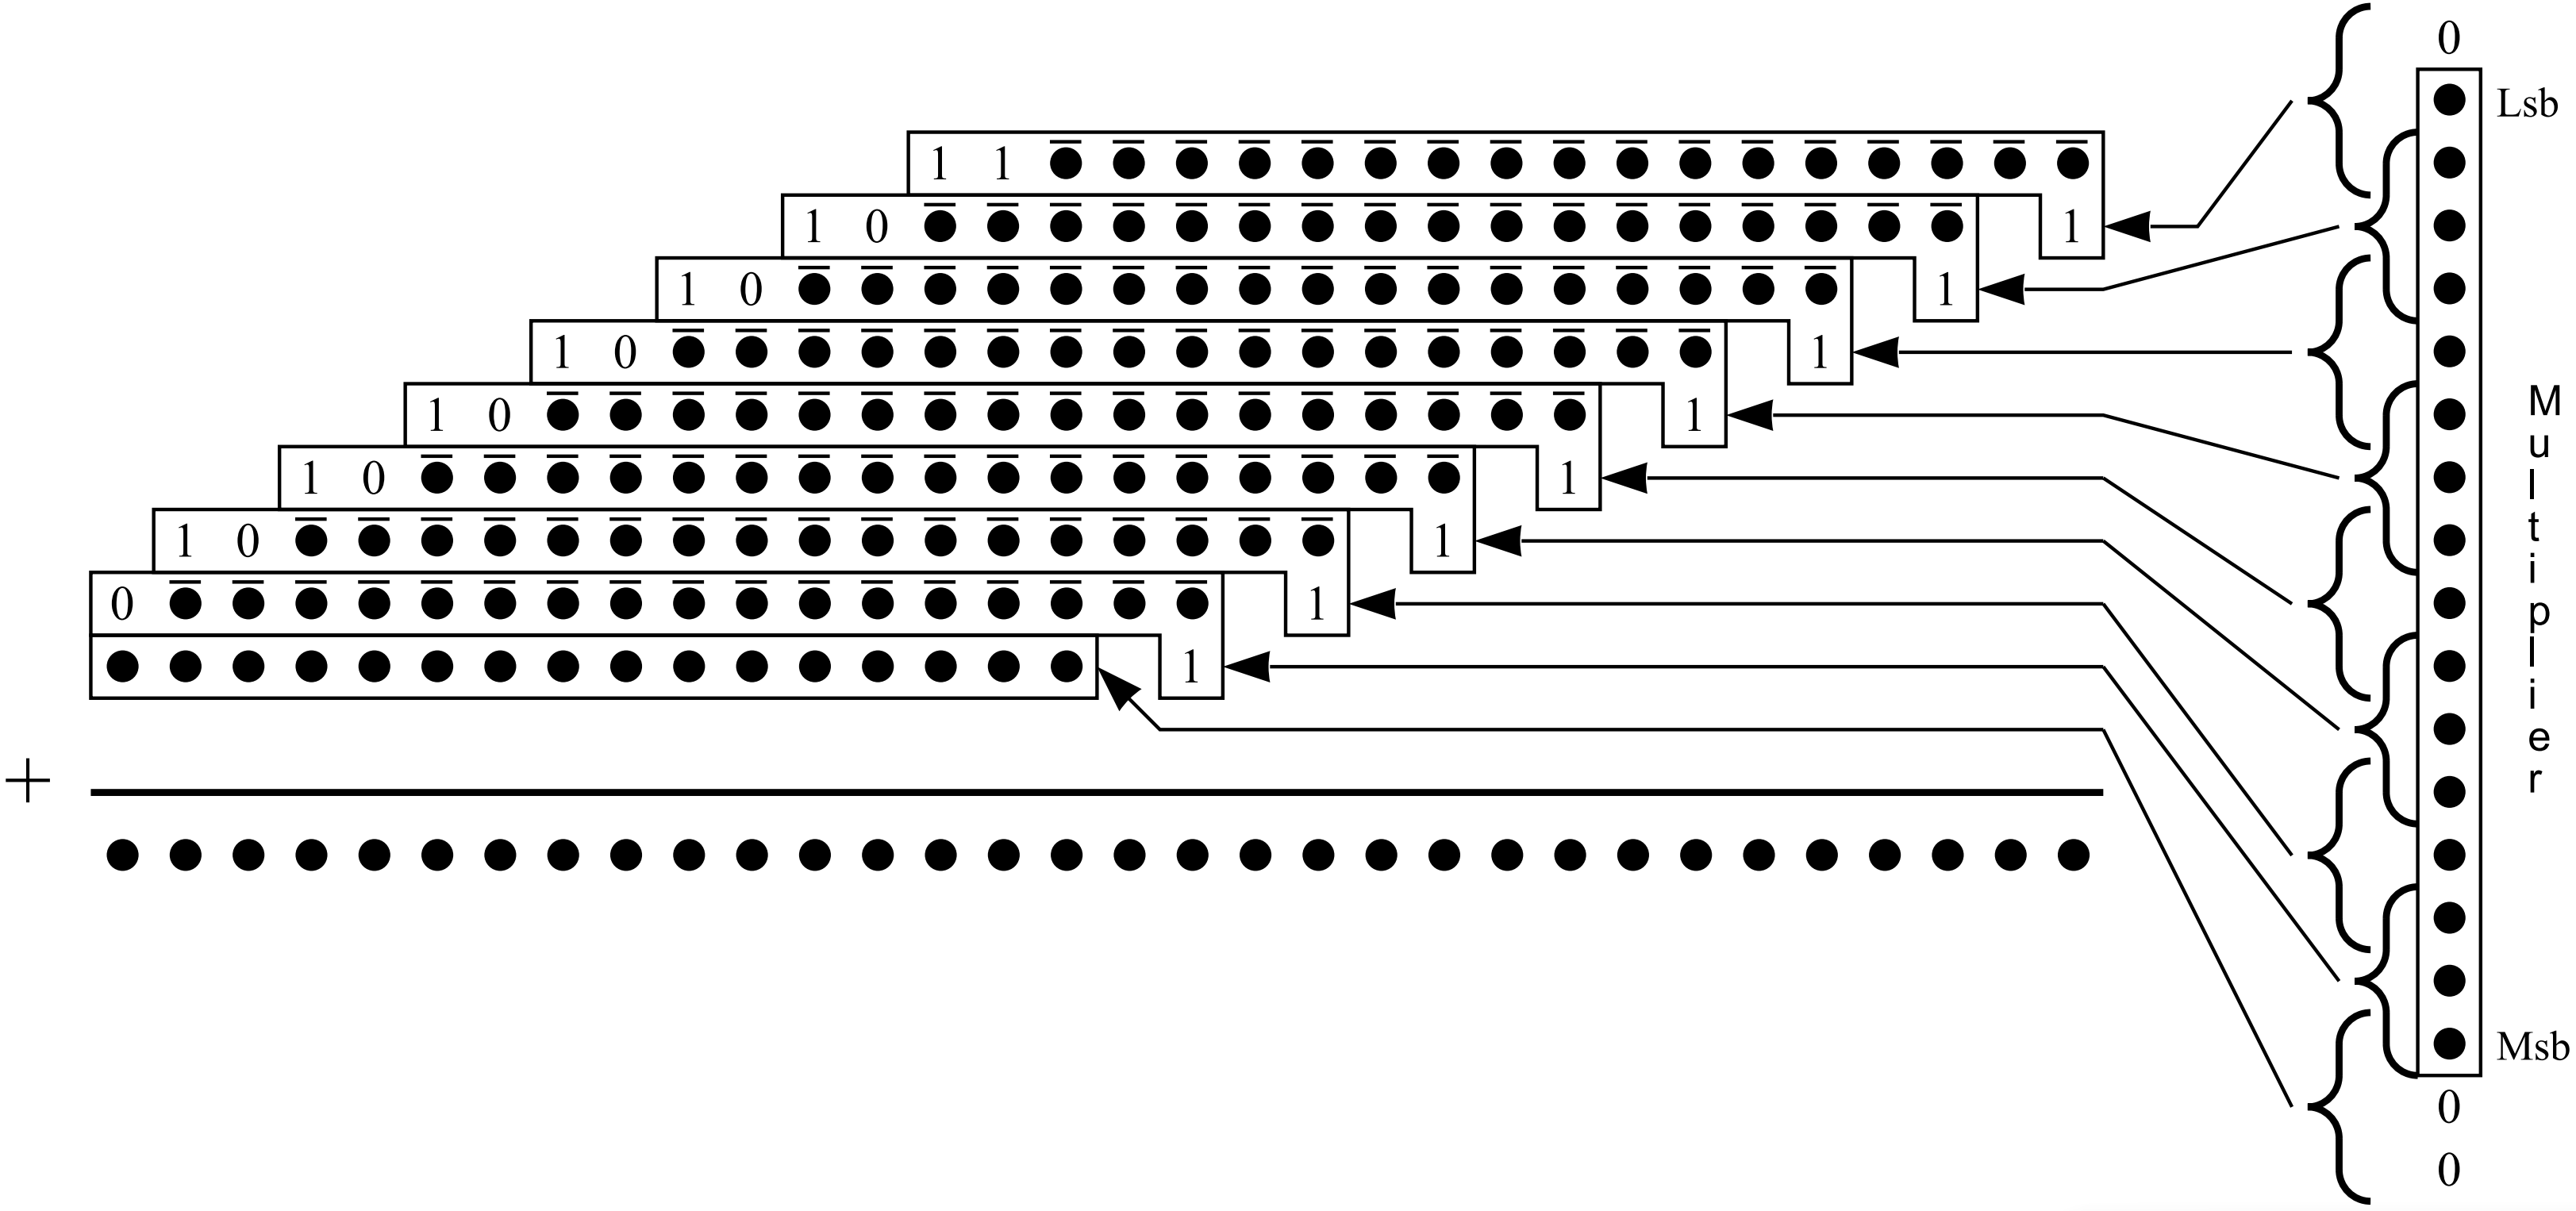
\includegraphics[width=\linewidth]{figs/EM-Fig-booth_unsign_negtive_summed.png}
    \end{minipage}
    }
    \subfigure[部分积正负均可的统一符号位扩展方法,$S$表示布斯码值的符号,$S=0$为正,$S=1$为负]{
    \label{EM:Fig:booth_16x16_unsign_PP_complete}
    \begin{minipage}[t]{0.48\linewidth}
    \centering
    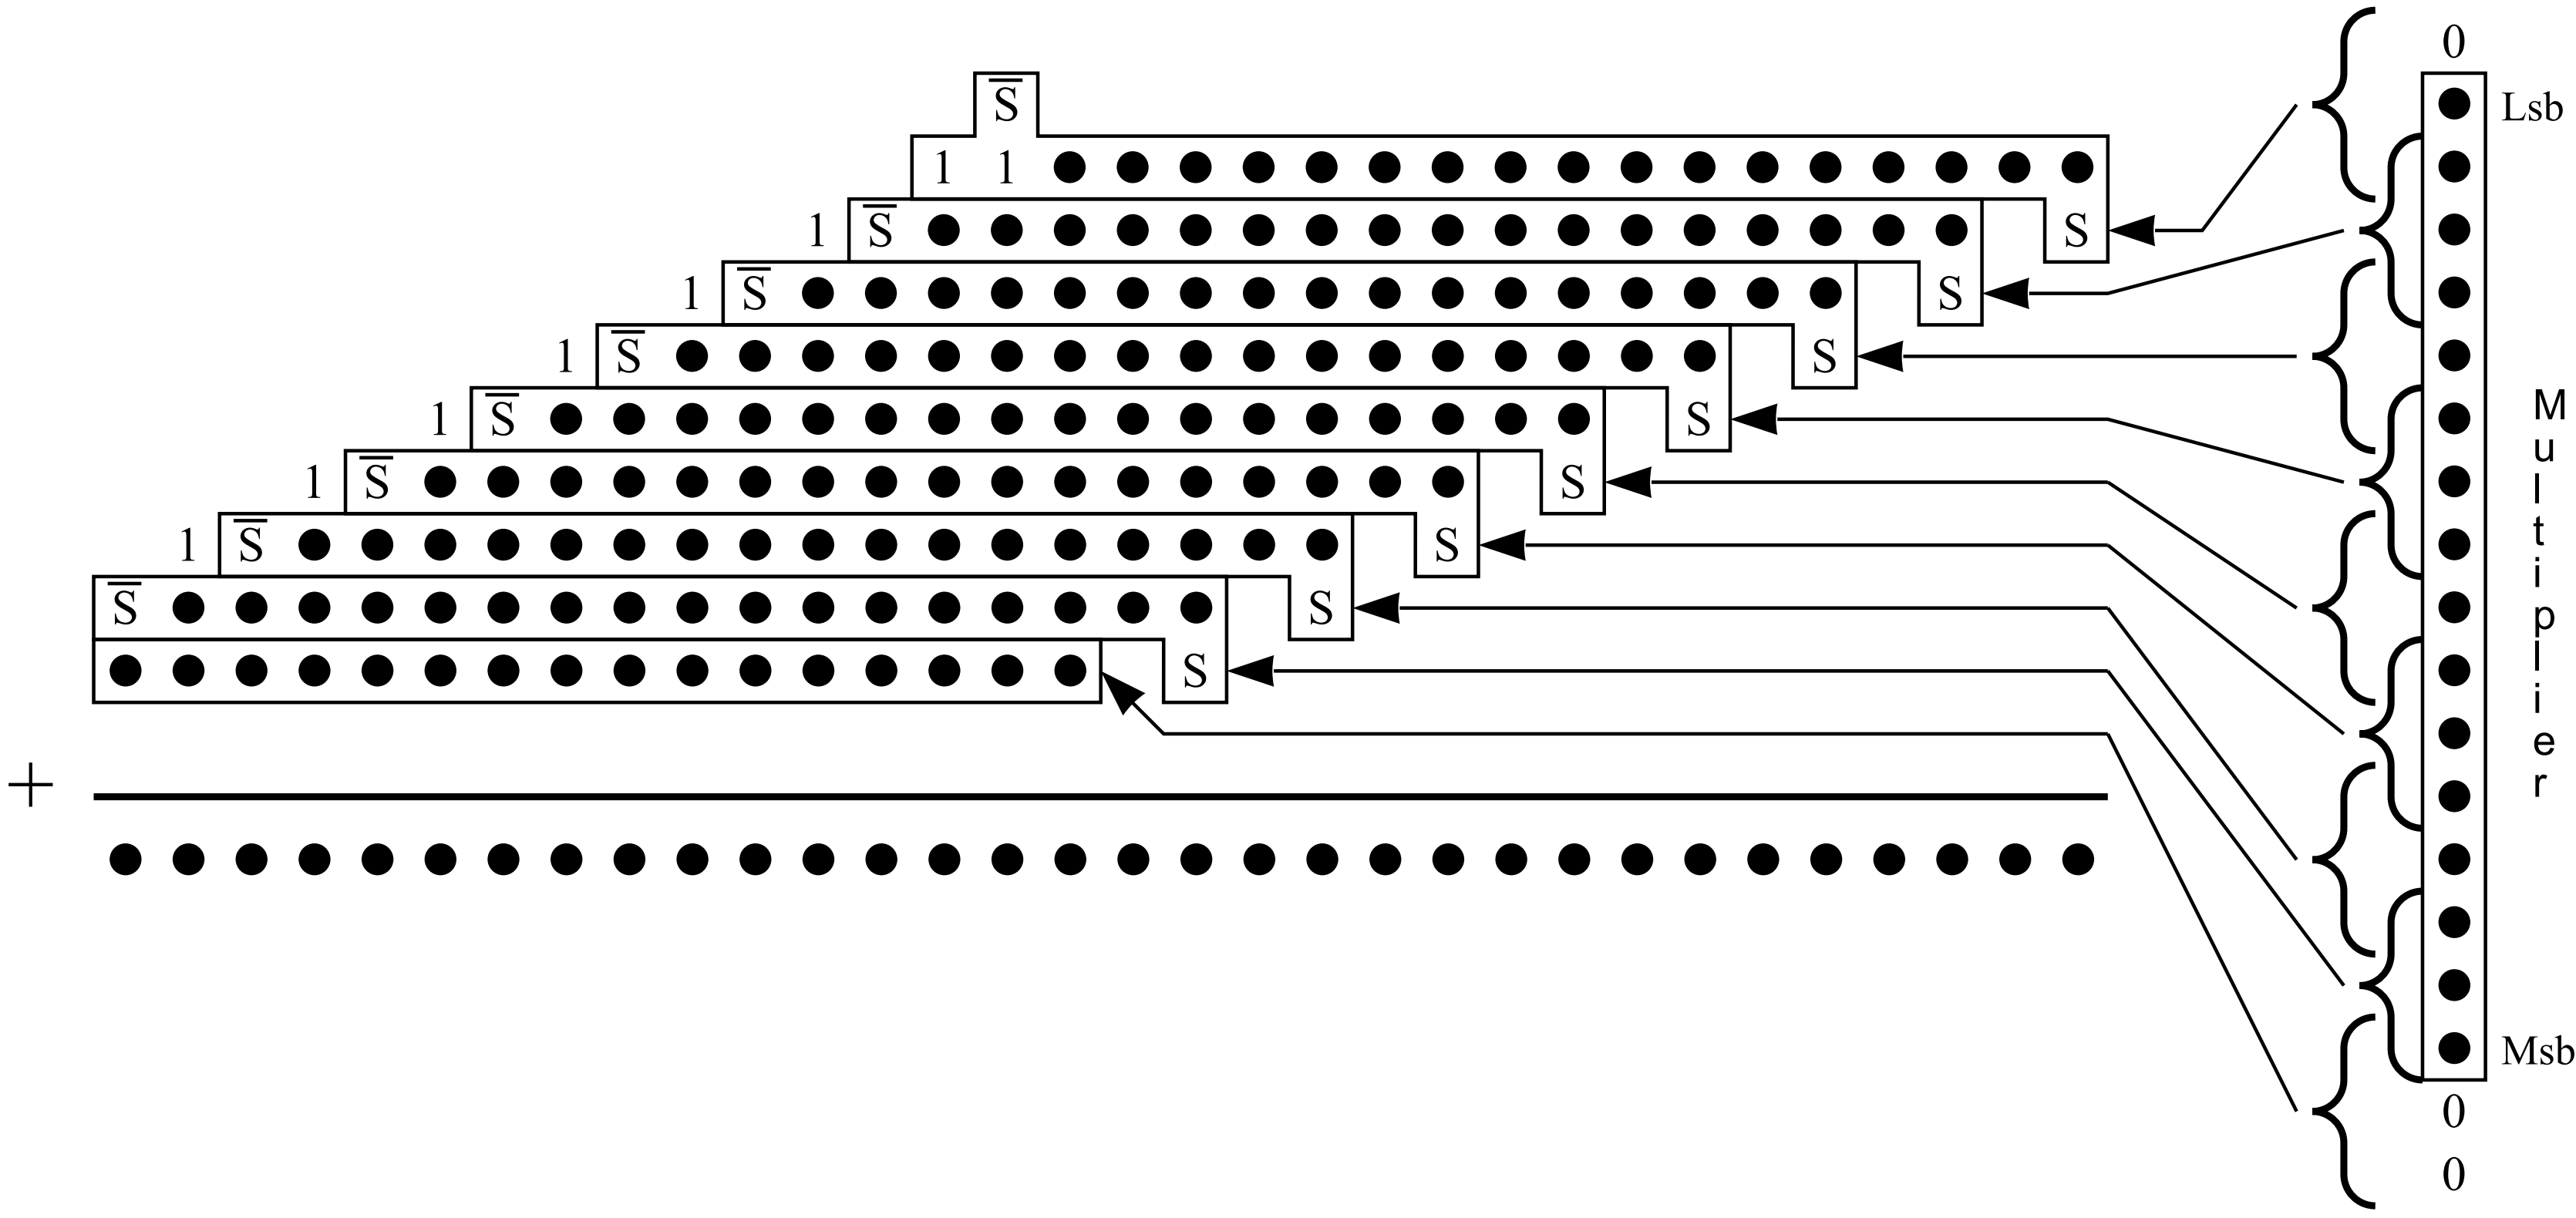
\includegraphics[width=\linewidth]{figs/EM-Fig-booth_unsign_complete.png}
    \end{minipage}
    }
    \subfigure[利用等价变换降低阵列层数后的部分积符号位扩展方法,$S$表示布斯码值的符号,$S=0$为正,$S=1$为负]{
    \label{EM:Fig:booth_16x16_unsign_PP_complete_reduce_height}
    \begin{minipage}[t]{0.48\linewidth}
    \centering
    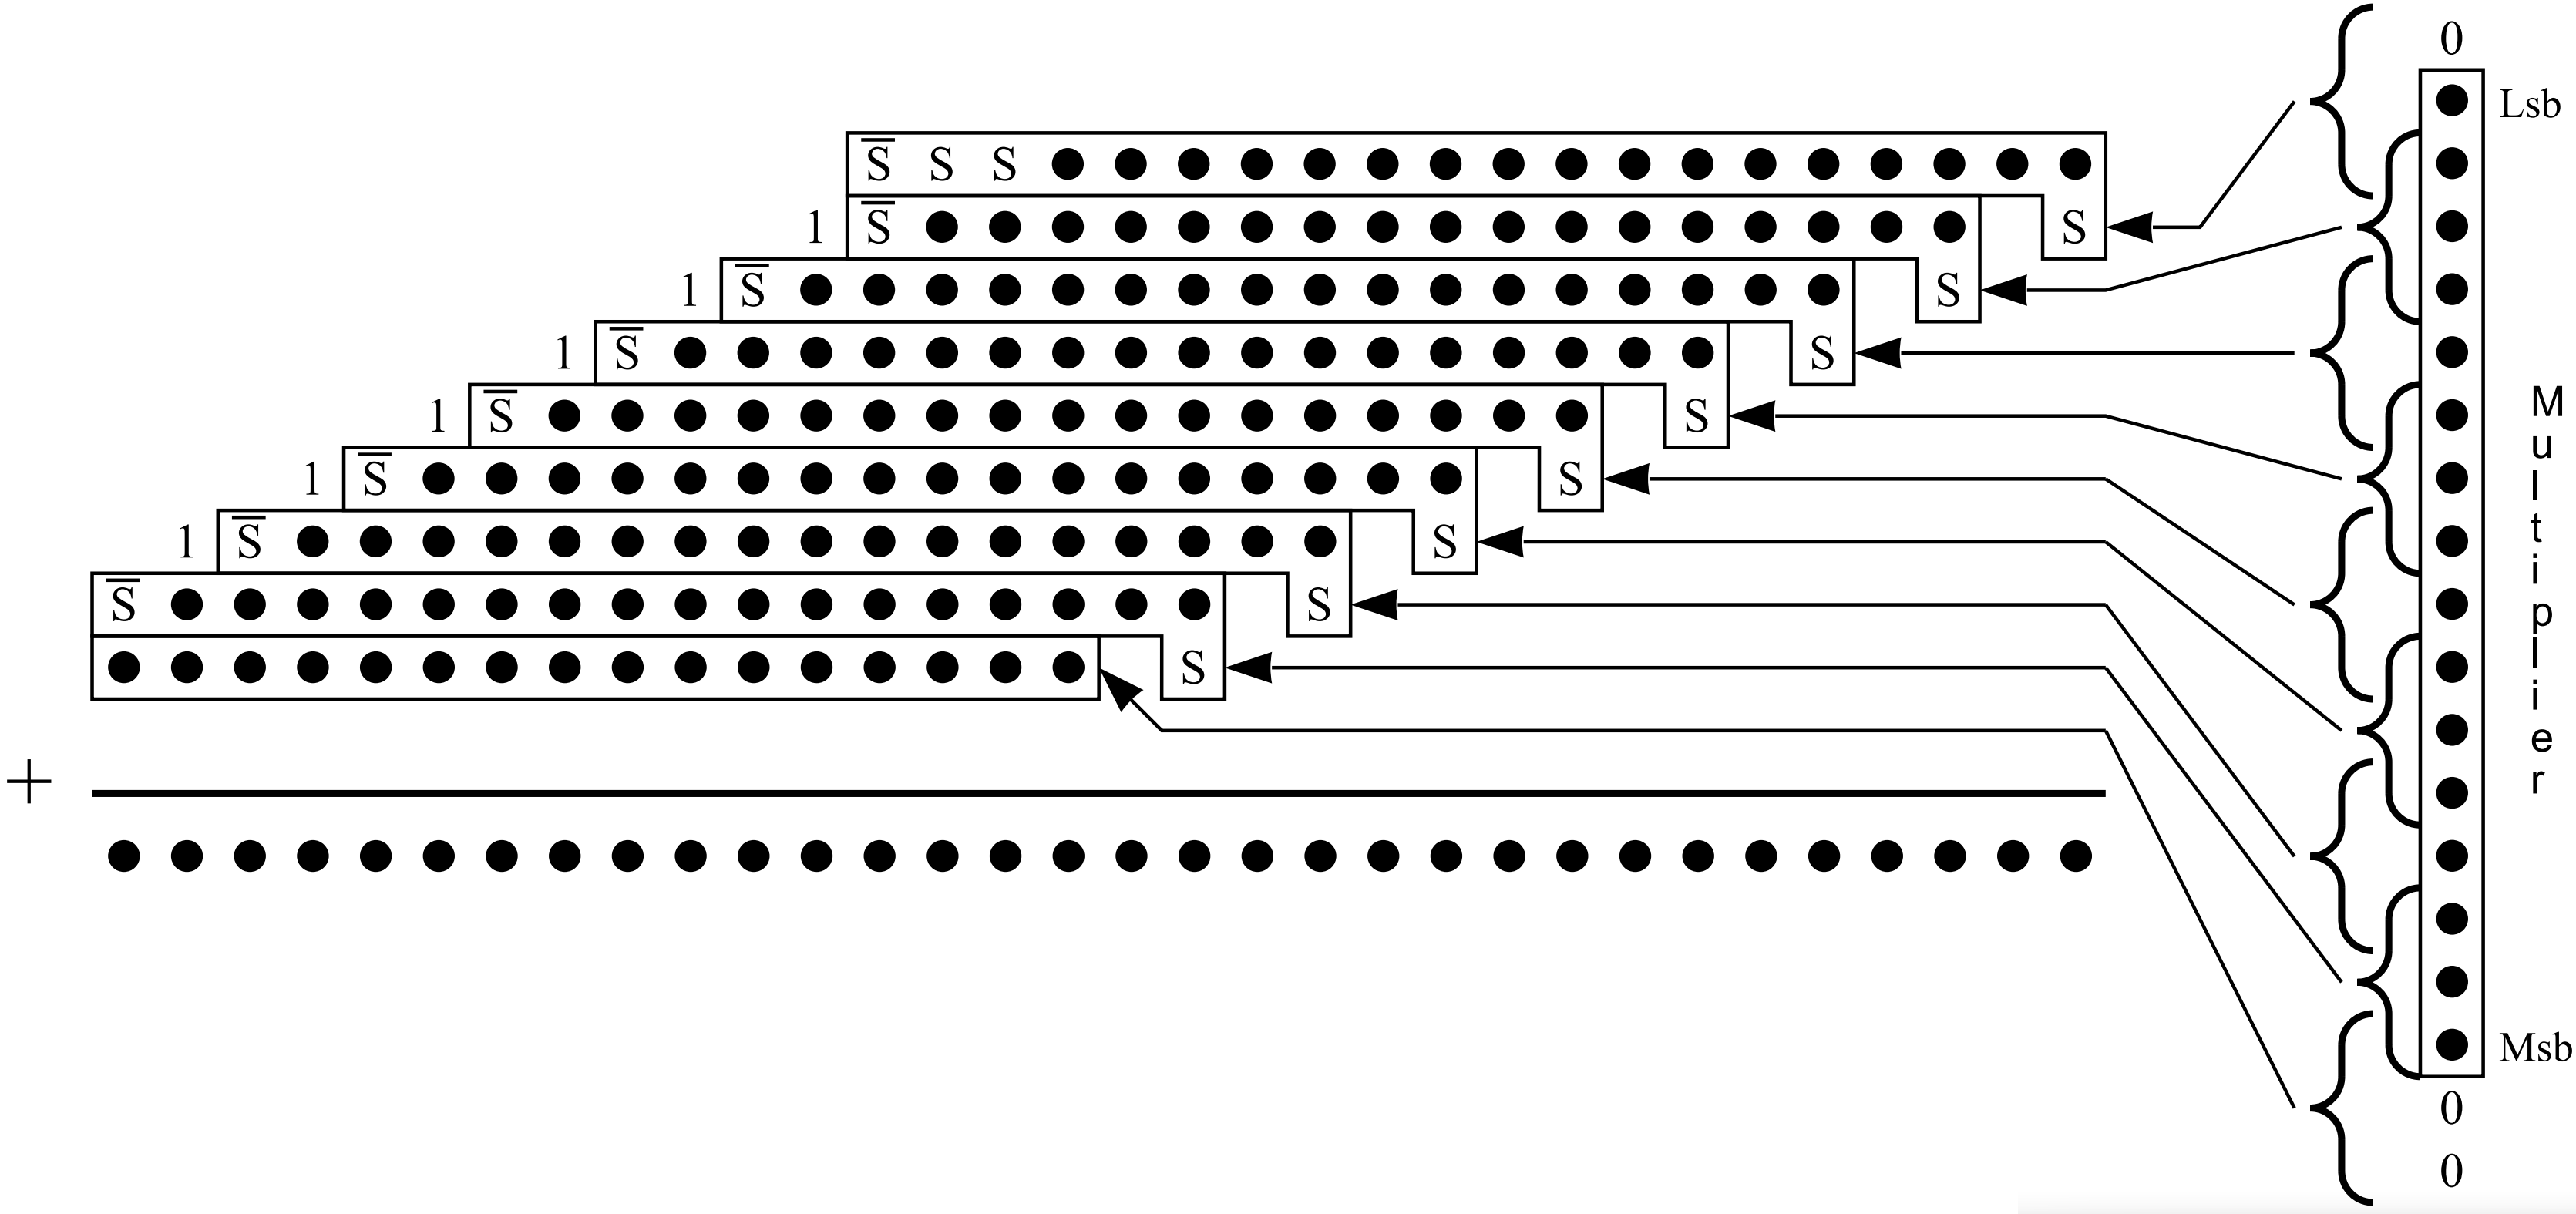
\includegraphics[width=\linewidth]{figs/EM-Fig-booth_unsign_complete_reduce_height.png}
    \end{minipage}
    }
\caption{$16\times16$无符号乘法的基4布斯算法部分积符号位扩展的改进办法}
\label{EM:Fig:booth_16x16_unsign_PP}
\end{figure}

对于$16\times16$无符号数乘法,假设每个部分积是非负数,高位应进行0扩展,0可省略,省略后的部分积阵列如图\ref{EM:Fig:booth_16x16_unsign_PP_positive}所示,部分积总数为$8+1 = 9$个。除了最下面的那个部分积之外,每个部分积的位宽均为17比特。不考虑最下面的那个部分积(该部分积永远是非负数),图\ref{EM:Fig:booth_16x16_unsign_PP_negtive}展示了所有部分积均为负数时的符号位扩展情况,即高位进行1扩展,对扩展产生的大量的1进行累加后的部分积阵列如图\ref{EM:Fig:booth_16x16_unsign_PP_negtive_summed}所示。
若图\ref{EM:Fig:booth_16x16_unsign_PP_negtive_summed}中存在部分积为正值,则需要对部分积的符号位进行修正,将高位的1扩展变回为0扩展,方法如图\ref{EM:Fig:booth_16x16_unsign_PP_complete}所示,引入$S$代表布斯码值的符号,$S=0$表示布斯码值为正,$S=1$表示布斯码值为负,达到对部分积进行统一符号位扩展的效果。最后,通过等价变换将\ref{EM:Fig:booth_16x16_unsign_PP_complete}中最上面的$\overline{S}$合并在部分积中,降低部分积阵列的层数,最终结果如图\ref{EM:Fig:booth_16x16_unsign_PP_complete_reduce_height}所示,即为16$\times$16无符号基4布斯算法的符号位扩展改进方法。

对于补码有符号布斯算法,当乘数的位宽为偶数时,部分积的个数会比同位宽的无符号布斯算法少一个。在符号位扩展方面的区别是,假设部分积均为负数而实际可能为正数、将大量的1累加后、需要对部分积的符号位进行修正时,不能单一的通过引入布斯码值的符号进行修正,而是要引入布斯码值的符号$S$和被乘数符号位的同或(Exclusive-NOR)进行修正。图\ref{EM:Fig:booth_16x16_signed_PP}展示了$16\times16$补码乘法的基4布斯算法部分积符号位扩展的改进方法示意图。
\begin{figure}[!htb]
    \centering
    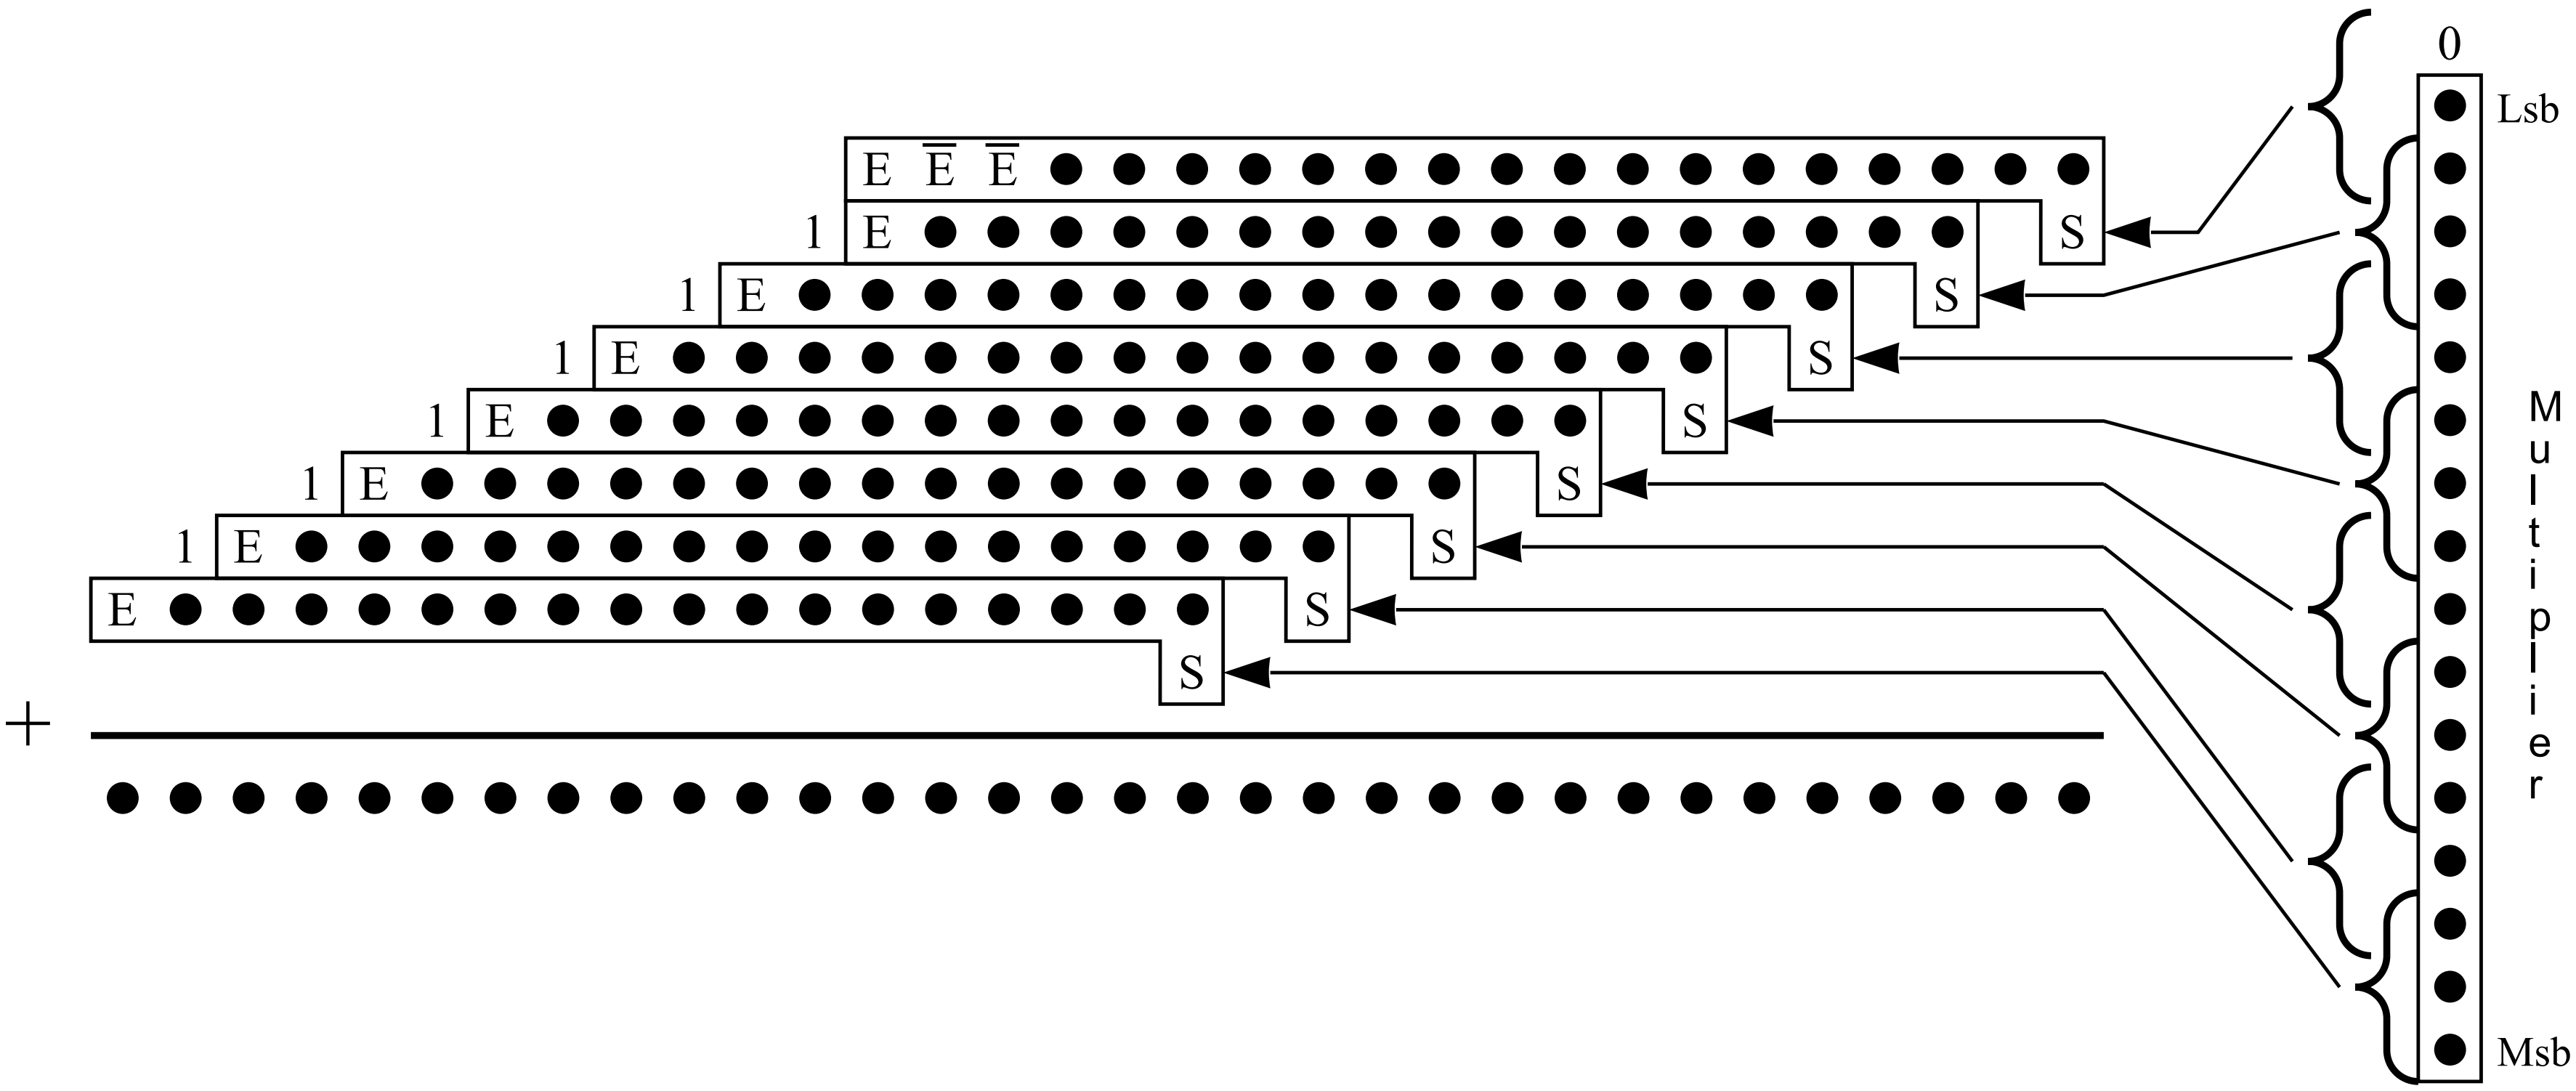
\includegraphics[width=\textwidth]{figs/EM-Fig-booth_signed.png}
    \caption{$16 \times 16$补码乘法的基4布斯算法部分积符号位扩展的改进方法,$E$表示布斯码值的符号$S$和被乘数符号位同或之后的结果}
    \label{EM:Fig:booth_16x16_signed_PP}
\end{figure}

\subsection{部分积的累加}

部分积产生后需要进行累加,这种累加本质上是一种多操作数的加法。一个直接的累加方式是用许多全加器(Full Adder, FA)组成阵列进行运算,被称为阵列累加,更为先进的方法是以进位保留或树结构的形式完成的。

\subsubsection{阵列累加}

\begin{figure}[!htb]
    \centering
    \subfigure[$4\times4$无符号数乘法产生的部分积]{
    \label{EM:Fig:array_multiplier_unsigned}
    \begin{minipage}[t]{0.48\linewidth}
    \centering
    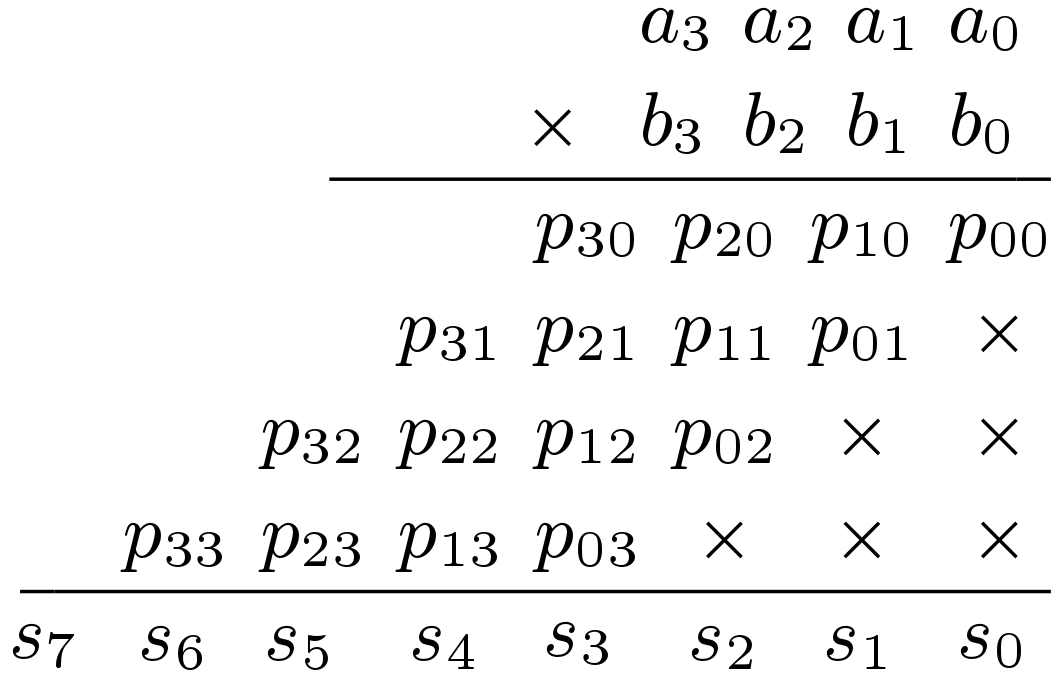
\includegraphics[width=\linewidth]{figs/EM-array_multiplier_unsigned.png}
    \end{minipage}
    }
    \subfigure[部分积的阵列累加电路]{
    \label{EM:Fig:array_multiplier_FA}
    \begin{minipage}[t]{0.48\linewidth}
    \centering
    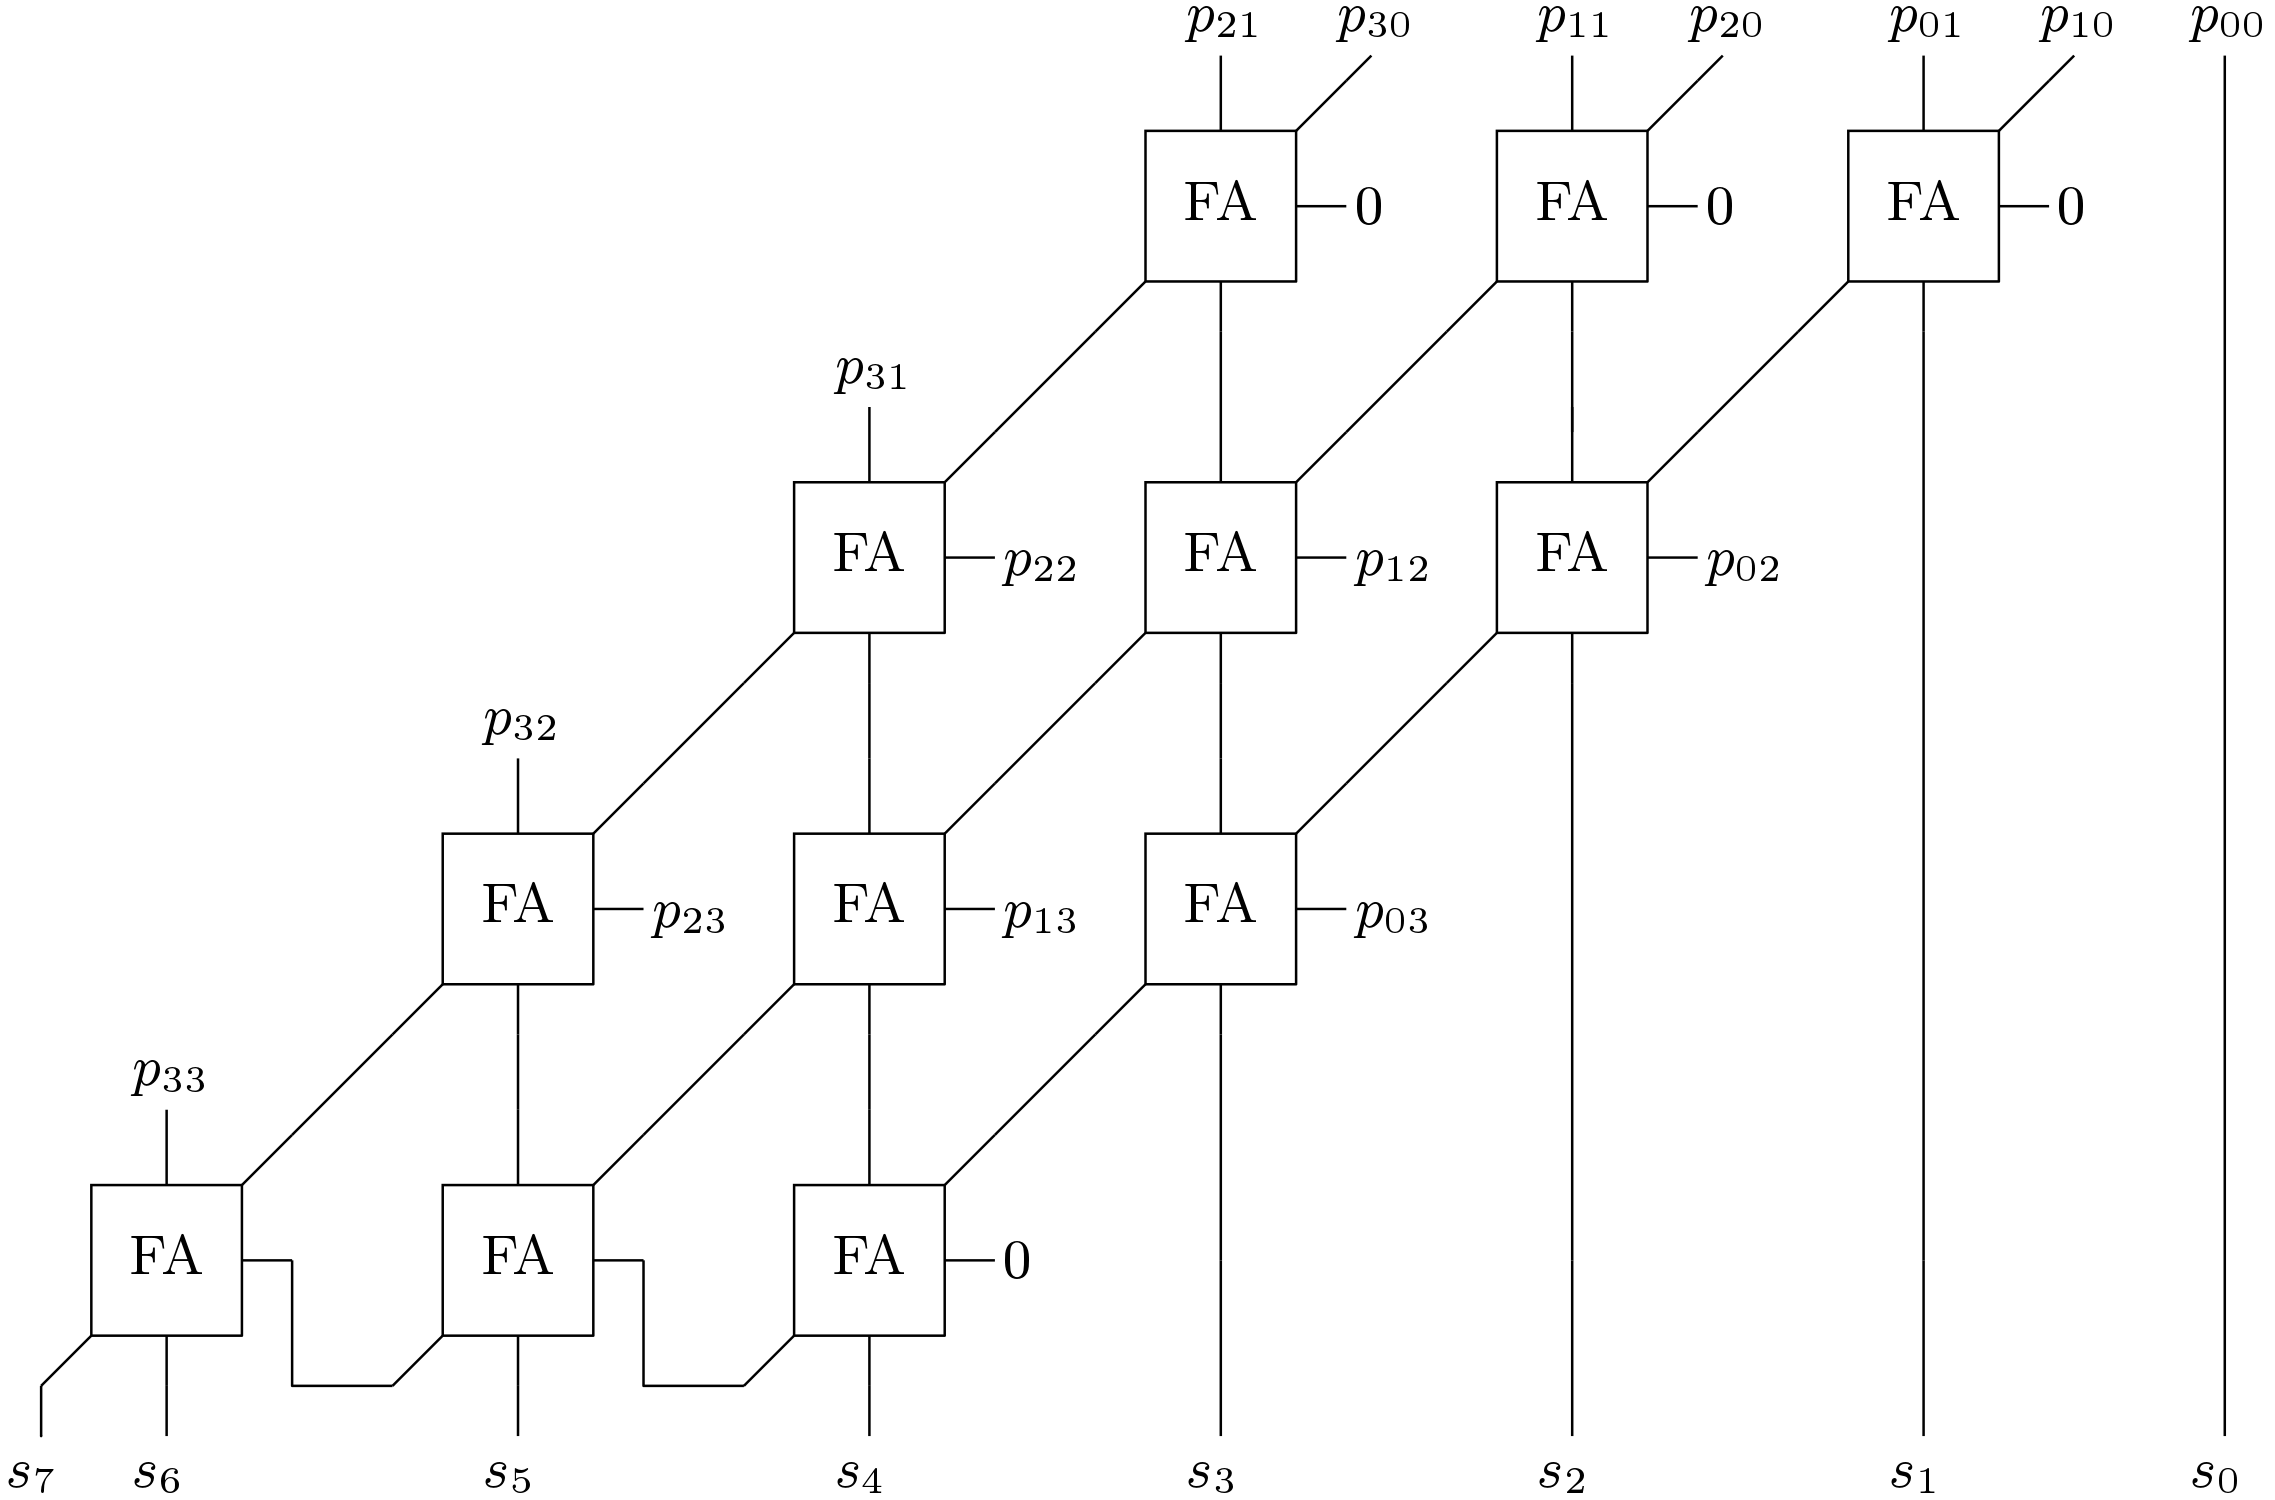
\includegraphics[width=\linewidth]{figs/EM-array_multiplier_FA.png}
    \end{minipage}
    }
\caption{$4\times4$无符号数乘法部分积及对应的阵列累加电路示意图}
\label{EM:Fig:array_multiplier}
\end{figure}

图\ref{EM:Fig:array_multiplier}展示了一个$4\times4$无符号数乘法部分积的生成及阵列累加电路示意图,部分积的移位操作通过布线即可完成,整个结构可以被很轻易的压缩成一个矩形,使得版图非常紧凑。阵列累加可以直接生成最终结果,并不需要最终相加这一步操作。然而,阵列累加结构中部分积的相加是通过逐位进位实现的,关键路径较长,性能较差。

\subsubsection{进位保留加法器}

进位保留加法器(Carry Save Adder, CSA)可以高效的对多个(通常是3个及以上)二进制数进行求和,通常用于乘法器中部分积的累加。在二进制中,两个或三个比特相加产生的进位不会超过1,基于此发现,CSA的基本思想是通过全加器将进位信号和求和信号保存下来,不断累加,直到将部分积压缩为两行,通过一个向量合并加法器得到最终结果。图\ref{EM:Fig:CSA}展示了一个4操作数8比特位宽,最后通过超前进位加法器进行向量合并的CSA结构图。
\begin{figure}[!htb]
    \centering
    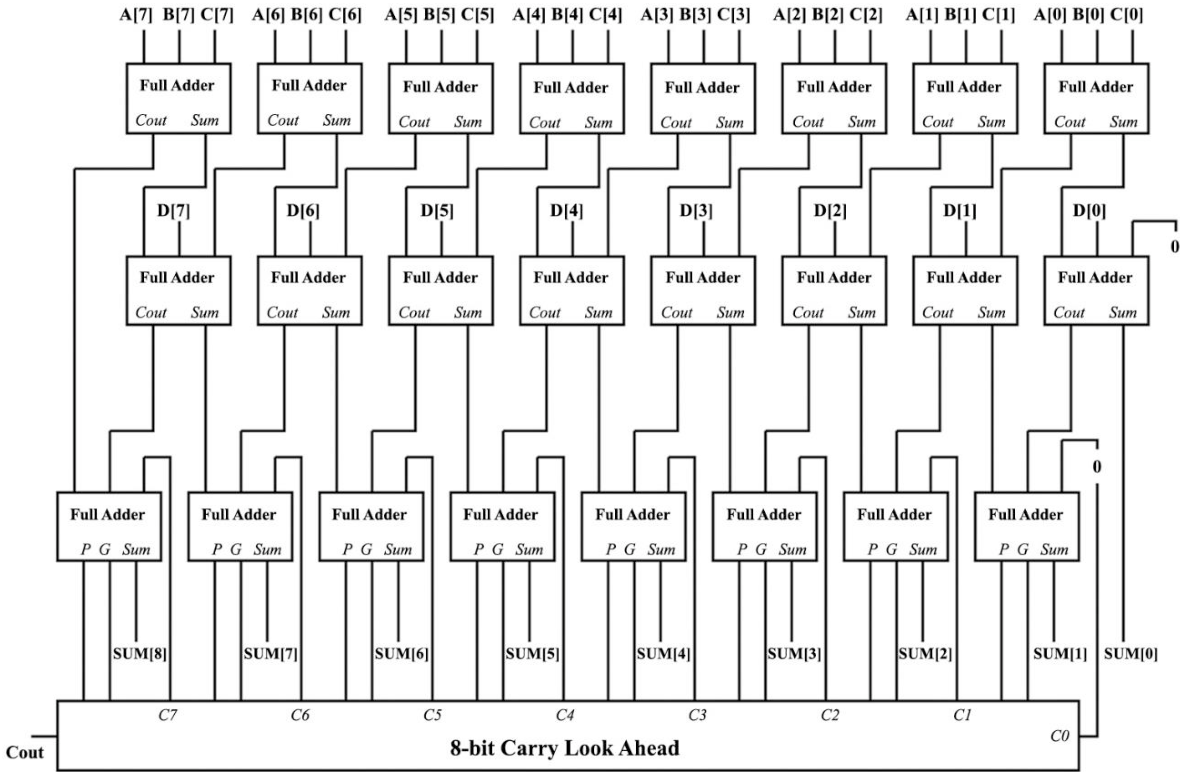
\includegraphics[width=0.85\textwidth]{figs/EM-CSA.png}
    \caption{4操作数8比特位宽,最后通过超前进位加法器相加的CSA结构图}
    \label{EM:Fig:CSA}
\end{figure}
从图中可以看到,4个8比特位宽的操作数经过两级全加器的运算变成了2个操作数,其中第一级全加器产生了$A$、$B$和$C$的进位及求和,之后和$D$一起被第二级全加器进行压缩,最后送给向量合并加法器进行求和。与阵列累加相比,CSA累加部分积的速度更快,性能更高。
注意这里的CSA并不会对操作数进行分组后并行累加,而是逐级累加\cite{数字集成电路_第十一章_设计运算功能块},这点与接下来讲的树形加法器有本质区别%
\IfStrEq{\Version}{Open}{%
    \footnote{\url{https://blog.csdn.net/qq_26707507/article/details/106146612}}。
}{。}

\subsubsection{树形加法器}

不论是阵列累加还是CSA累加本质上都是通过排列全加器实现的,全加器也可以安排为树形,这样既能减少累加电路所需的全加器的数量,还能降低关键路径延迟。树形加法器的实现可以看作是并行的进位保留加法器,累加效率更高。常见的树形加法器包括华莱士树\cite{EM:Wallace}和达达树\cite{EM:Dadda}。

(1)华莱士树 \label{华莱士树}

华莱士树(Wallace tree)加法器\cite{EM:Wallace}是由澳大利亚计算机科学家克里斯·华莱士(Christopher Stewart Wallace)于1964年设计的,被广泛用于乘法器中部分积的高效快速累加。其基本步骤如下:(a)假设所有部分积都是同时生成的,第一步是将部分积每3个分为一组(不足3个保持),并将每组部分积的个数通过全加器和半加器压缩为2个;(b)重复对部分积进行分组并压缩,直到只剩下两个部分积;(c)相加最后两个部分积得到最终结果。
\begin{figure}[!htb]
    \centering
    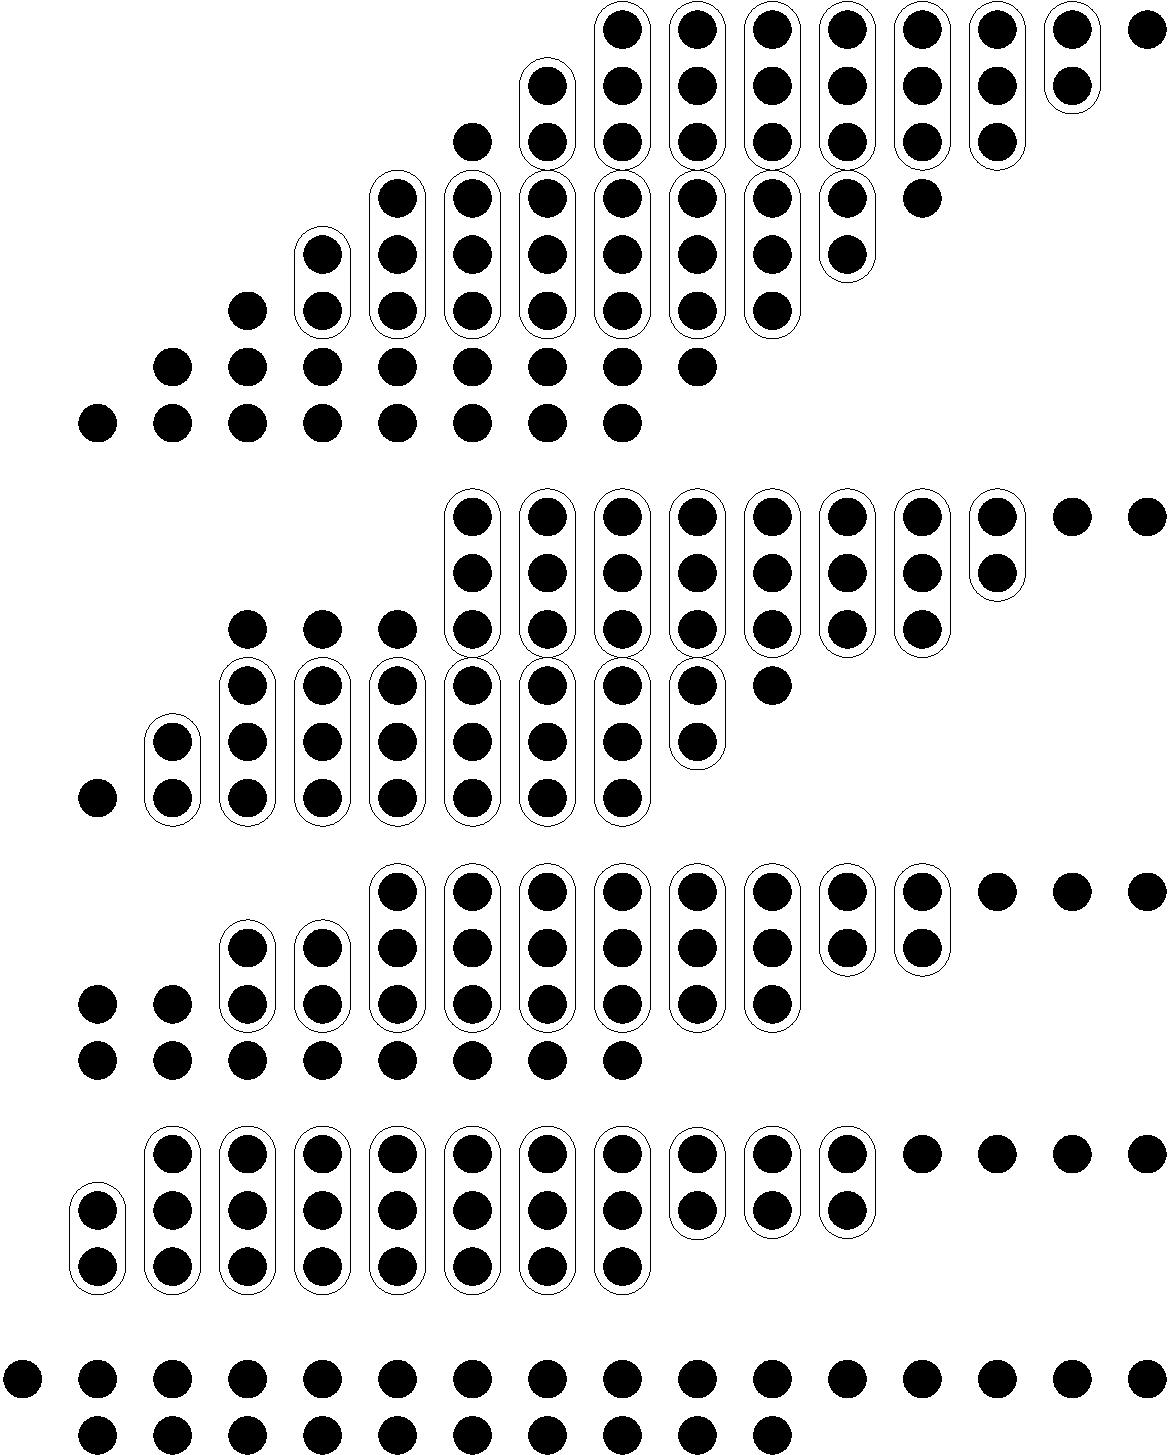
\includegraphics[width=0.85\textwidth]{figs/EM-wallace.pdf}
    \caption{利用华莱士树加法器对$8 \times 8$无符号数乘法部分积进行累加的示意图}
    \label{EM:Fig:wallace}
\end{figure}
图\ref{EM:Fig:wallace}展示了一个利用华莱士树加法器对$8 \times 8$无符号数相乘产生的部分积进行累加的过程示意图,每个点表示一个比特,每个圈代表一个全加器或半加器(包含两个点的圈代表半加器,包含三个点的圈代表全加器),一共分组并压缩了4次,消耗了15个半加器和38个全加器,将8个部分积变成了2个部分积,改进的华莱士树方法能够使用更少的半加器,降低设计的复杂度\cite{EM:redeuce_wallace}。
与阵列累加方法和进位保留方法相比,华莱士树加法器的速度很快,且位宽越大越明显,但缺点是电路结构非常不规则,难以获得高质量的版图设计。全加器本质上是一个3:2压缩器,能够将乘法器中每组部分积的数目减少至三分之二,利用4:2甚至更高比例的压缩器,基于华莱士树方法可以得到性能更高的乘法器\cite{EM:wallace_42}。

(2)达达树

达达树(Dadda tree)加法器是由计算机科学家Luigi Dadda于1965年发明的一种树形加法结构\cite{EM:Dadda},与华莱士树方法类似,达达树也是采用全加器和半加器对部分积进行压缩,直到只剩下两个部分积。区别在于,Luigi Dadda对华莱士树进行了重构,在树的级数(深度)不变的情况下使用了数量更少的全加器和半加器,节省了硬件资源,但缺点是最后两个部分积的位宽可能会稍大。具体步骤如下%
\IfStrEq{\Version}{Open}{%
    \footnote{\url{https://en.wikipedia.org/wiki/Dadda_multiplier}}:
}{:}
\begin{itemize}
    \item 部分积的累加过程由一个正整数序列$d_j$来控制:$d_1=2$,$d_{j+1}=\lfloor 1.5 \rfloor d_j$,$\lfloor \ \rfloor$表示向下取整;
    \item 初始的$j$应尽可能大并满足$d_j < n$,$n$是乘数的位宽(部分积阵列的高度);
    \item $j$逐步递减,且任意$j$下对部分积阵列从最低权重按列开始遍历:(a)若列高度小于或等于$d_j$,跳过该列;(b)若列高度等于$d_j+1$,运用半加器对该列最上面的两个比特进行运算,产生进位及求和;(c)若列高度大于$d_j+1$,运用全加器对该列最上面的三个比特进行运算,产生进位及求和,并对该列重复(a)、(b)、(c)的操作;注意进位会增加相邻高权重列的高度;
    \item 累加结束时$j=1$,$d_j=2$(部分积只有两行),之后使用一个向量合并加法器求得最终结果。
\end{itemize}

图\ref{EM:Fig:dadda}展示了一个运用达达树对$8 \times 8$无符号数乘法生成的部分积进行压缩的过程示意图,该树的深度与图\ref{EM:Fig:wallace}中的华莱士树的深度相同,但使用了更少的全加器和半加器:达达树使用了35个全加器、7个半加器,华莱士树使用了38个全加器、15个半加器。
\begin{figure}[!htb]
    \centering
    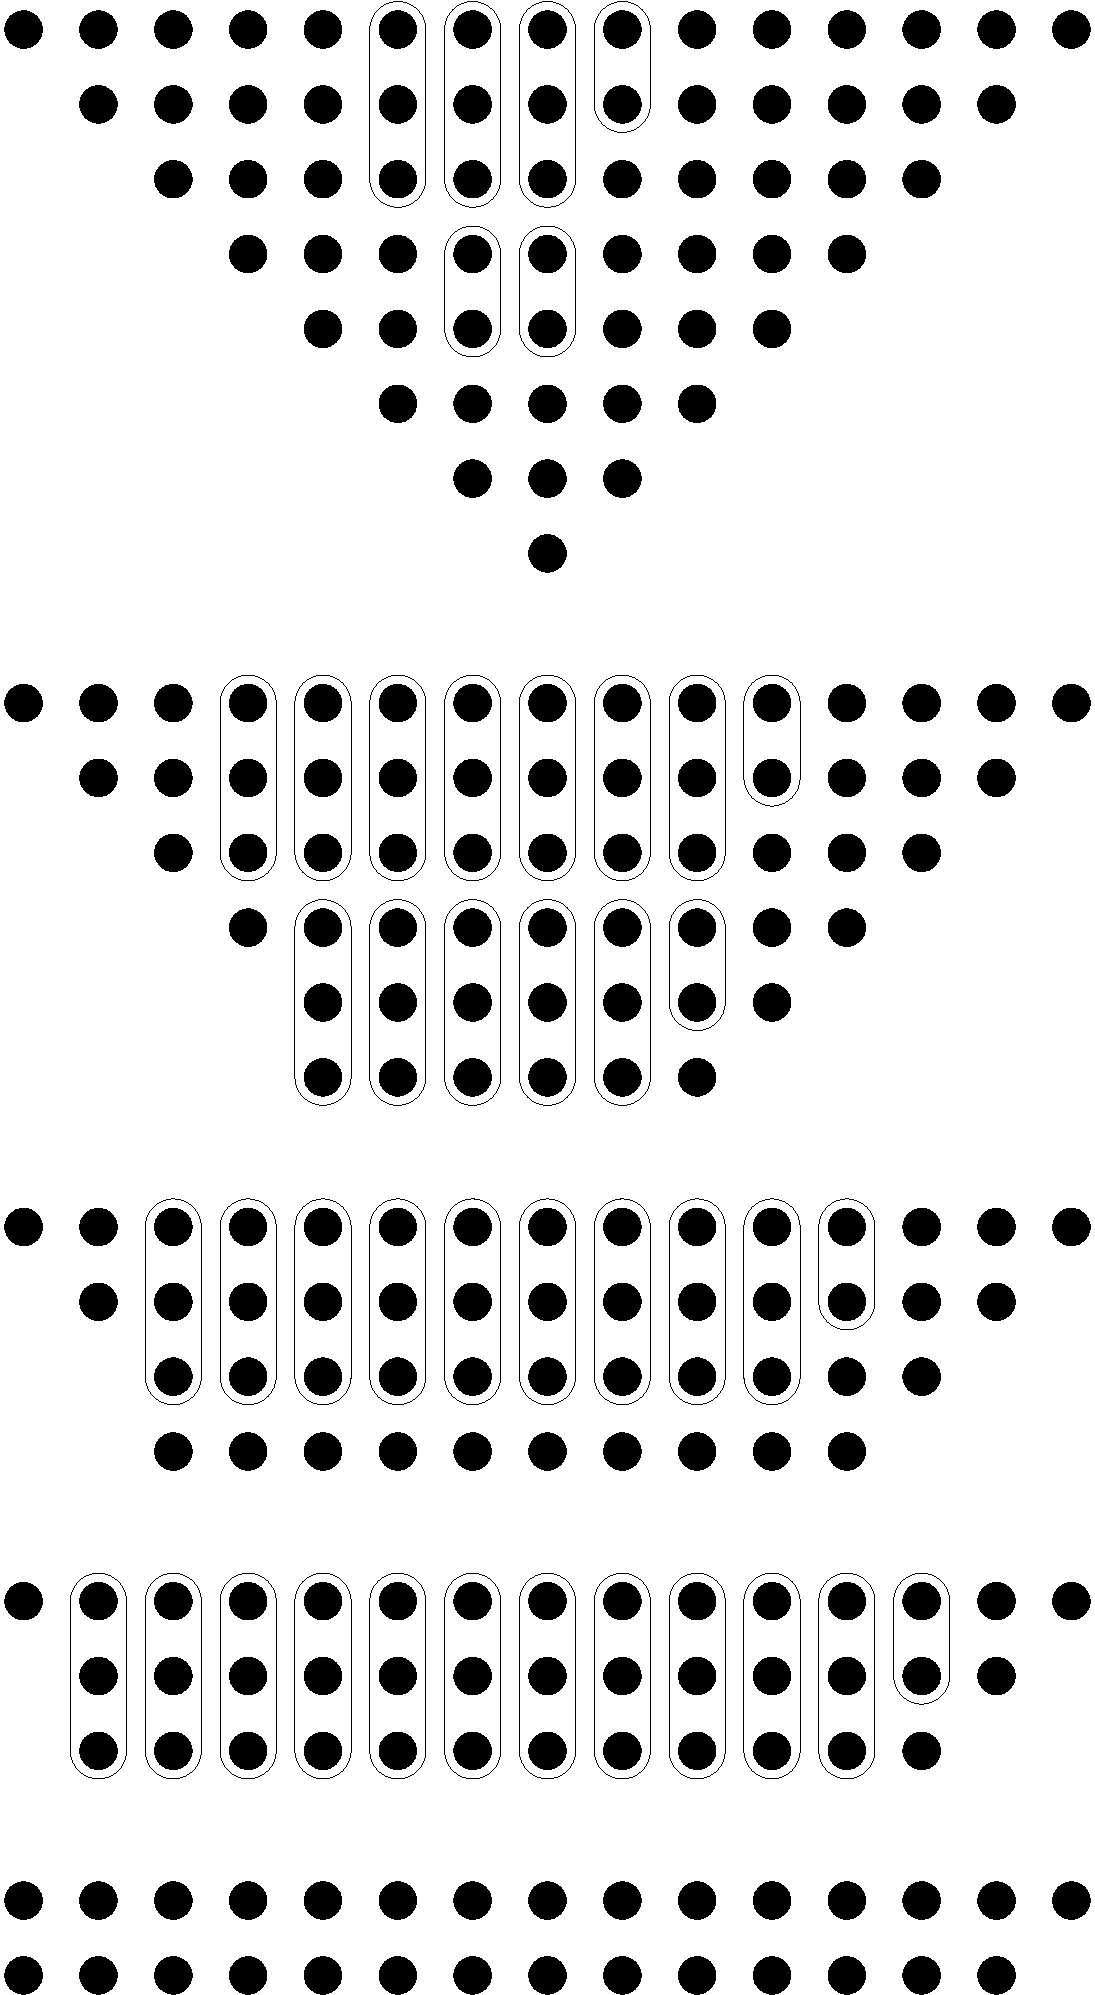
\includegraphics[width=0.7\textwidth]{figs/EM-dadda.pdf}
    \caption{利用达达树加法器对$8 \times 8$无符号数乘法部分积进行累加的示意图}
    \label{EM:Fig:dadda}
\end{figure}

\subsection{最终相加}

除了阵列累加方式以外,进位保存加法器、树形加法器等高速的部分积累加电路最后会产生两个部分积,需要一个向量合并加法器(Vector-Merging Adder, VMA)进行最终运算,目前常见的VMA有以下几种结构:

\subsubsection{行波进位加法器}

行波进位加法器(Ripple-Carry Adder, RCA)又被称为逐级进位加法器,是由一系列全加器级联而成,优点是面积小、占用资源少,缺点是速度慢、效率低。在最好情况下,任何位宽的RCA都不需要传递进位信号也可以得到正确结果;但在最坏情况下,得到最终结果的延迟会随着位宽的增加而线性增大,从而限制了系统的运算速度。

\subsubsection{超前进位加法器}

当加法器的位宽较大时,由于RCA在最坏情况下每一级全加器的计算必须等待前一级的进位输出,导致其关键路径较长,效率较低,超前进位加法器(Carry-Lookahead Adder)的思想是并行计算每一级全加器的进位输出,本质上是数学公式推导的结果,原理如下:

假设RCA中第$i$级全加器的输入为$a_i$、$b_i$、$c_{i}$,进位输出为$c_{i+1}$,设$p_i = a_i \oplus b_i$,$g_i = a_i b_i$,有:
\begin{equation}
\begin{aligned}
    c_{i+1} = & \ a_i b_i + c_i(a_i \oplus b_i) \\
    = & \ g_i + c_i p_i
\end{aligned}
\label{EM:Eq:CLA}
\end{equation}
若$p_i=1$,则$g_i =0$,$c_{i+1}=c_i$,若$p_i=0$,则$c_{i+1}=g_i$,因此$p_i$和$g_i$分别被称为第$i$级加法器的传播信号和生成信号。
对$c_{i}, c_{i-1},c_{i-2},\cdots,c_{1}$使用式\eqref{EM:Eq:CLA},可将$c_{i+1}$的求解转换为输入数的逻辑操作(假设$c_0=0$),避免了RCA中的进位依赖问题,实现了效率的提升。与RCA相比,CLA的关键路径短,速度快,但在加法器位宽较大时,CLA中高位的进位输出表达式涉及的变量较多,存在较大扇入扇出的问题。同时,组合逻辑电路的输入信号过多也会引起竞争冒险(Race hazard),产生毛刺(Glitch),影响系统的稳定性。所以在加法器的位宽较大时,要想利用CLA提高进位效率,通常会先对操作数进行划分,对每个部分实行CLA,CLA之间再通过级联或嵌套等方式进行连接%
\IfStrEq{\Version}{Open}{%
    \footnote{\url{https://zhuanlan.zhihu.com/p/378267920}},
}{,}
以避免大输入位宽逻辑门的产生。其中,采用级联对各CLA块之间进行连接的方式被称为分块CLA,采用嵌套对各CLA块之间进行连接的方式被称为分级CLA。
灵活地对操作数进行划分并嵌套,能够得到许多不同的CLA结构,可在面积和速度之间进行权衡,存在一套能够简洁表示各种分级超前进位结构的符号体系,具体内容在后面的并行前缀加法器中详细讲述。
最后需要注意的是,基于CLA方法实现的加法器的面积和复杂度通常会比同位宽的RCA大。

\subsubsection{进位旁路加法器}

基于式\eqref{EM:Eq:CLA}可以看到,一个$n$位RCA的最坏情况发生在$p_{n-1}, p_{n-2}, \cdots, p_0$均为1的时候(即$p_{n-1} p_{n-2} \cdots p_0=1$),此时$g_{n-1}, g_{n-2}, \cdots, g_0$均为0,式\eqref{EM:Eq:CLA}变为:
\begin{equation}
    c_{i+1} =  c_i
\label{EM:Eq:CSKA_prop}
\end{equation}
进位旁路加法器(Carry-Skip Adder,为了与进位保存加法器区分,这里缩写为CSKA,也叫Carry-bypass adder)的思想便是加速该情况下进位链的传播。一个$n$位的CSKA包括一个$n$位的RCA、一个$n$位的多输入与门(AND)、以及一个二选一的多路选择器(Multiplexer, MUX)。图\ref{EM:Fig:CSKA_4bit}展示了一个4比特CSKA的结构图,$p_0 \sim p_3$信号通过与门连接到MUX上作为选择信号,当$p_0 p_1 p_2 p_3=1$时,$c_0$通过MUX直接输出,中间的RCA被旁路掉,大大减少了延迟。
\begin{figure}[!htb]
    \centering
    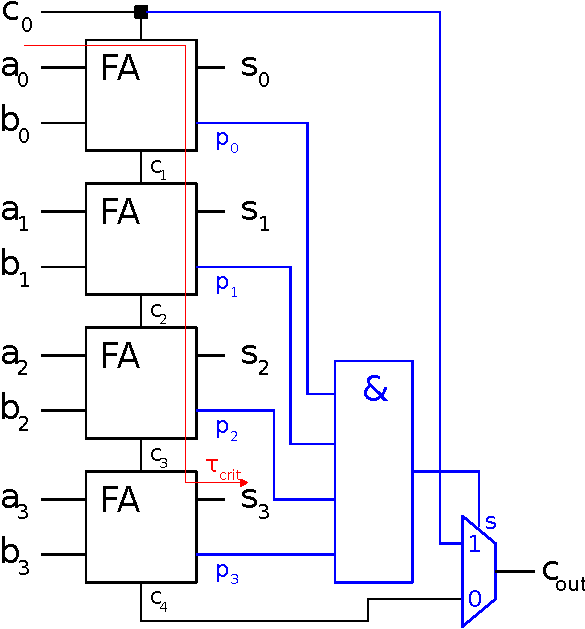
\includegraphics[width=0.4\textwidth]{figs/EM-CSKA_4Bit.pdf}
    \caption{一个4比特CSKA的结构示意图,FA代表全加器}
\label{EM:Fig:CSKA_4bit}
\end{figure}

但是,与RCA相比,CSKA并没有明显的性能改进(如图\ref{EM:Fig:CSKA_4bit}中的关键路径$\tau_{\text{crit}}$同样需要经过4个全加器)。因此,当位宽较大时,采用分块CSKA(Block CSKA)的办法才能取得较为显著的速度增益。若一个$n$比特的分块CSKA有$m$块CSKA,每块CSKA的位宽均为$\dfrac{n}{m}$,则该分块CSKA被称为固定大小分块CSKA%
\IfStrEq{\Version}{Open}{%
    \footnote{\url{https://en.wikipedia.org/wiki/Carry-skip_adder}}。
}{。}
\begin{figure}[!htb]
    \centering
    \includegraphics[width=\textwidth]{figs/EM-CSKA_16Bit.pdf}
    \caption{一个固定大小分块CSKA的例子:通过级联4个4比特CSKA实现16比特加法}
\label{EM:Fig:CSKA_16bit}
\end{figure}

图\ref{EM:Fig:CSKA_16bit}展示了一个通过级联4个4比特CSKA实现的16比特固定大小分块CSKA加法器的结构图,其关键路径(红色线条$\text{T}_{\text{critical}}$)延迟包括头尾两个4比特RCA的延迟和中间两个旁路逻辑中MUX的延迟。从静态时序分析(Static Timing Analysis, STA)的角度看,图\ref{EM:Fig:CSKA_16bit}的关键路径延迟比一个16比特的RCA更差,但STA得到的关键路径是伪路径,电路实际运行过程中并不会发生。固定大小分块CSKA真实的关键路径可通过以下过程来理解:输入同时到来后,每块CSKA很快地被确定为是否处于旁路状态;之后所有的CSKA同时计算,假设首块CSKA没有被旁路,那么当首块CSKA的进位输出得到后,后面所有的CSKA要么处于旁路状态、要么也已计算完毕。
因此固定大小分块CSKA的最坏情况是,进位信号需要通过首尾两个RCA和中间全部处于旁路状态的CSKA中的MUX。通过调整块的大小和层级,分块CSKA的性能可得到进一步地优化。
最后需要注意的是,与其他快速加法器如CLA不同,分块CSKA的性能仅在输入是某些情况下会获得提高,即速度的提高是概率性的。

\subsubsection{进位选择加法器}

另一种避免出现RCA中最坏情况下逐级进位的方法是预先考虑进位输入的两种可能的值(0和1),并提前计算针对这两种可能性的结果,一旦进位输入的值确定,正确的结果可以通过一个简单的MUX选出,这一设想的实现被称为进位选择加法器(Carry-Select Adder,为了与进位保存加法器区分,这里缩写为CSEA)。CSEA通常只包括RCA和MUX,一个4比特位宽的CSEA的结构如图\ref{EM:Fig:CSEA_basic}所示,由于一个RCA的进位为0,而另一个RCA的进位为1,因此可通过实际进位输入决定哪个RCA的结果作为输出,与同位宽的RCA相比,除了MUX以外,CSEA消耗了两倍数量的全加器,是面积换性能的典型代表。
\begin{figure}[!htb]
    \centering
    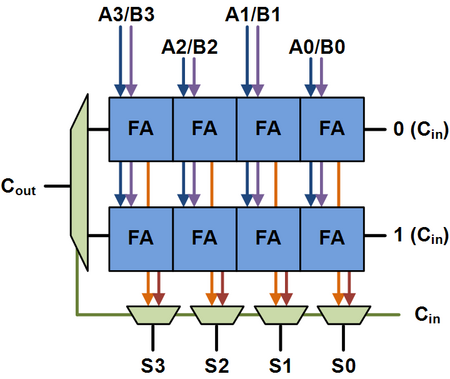
\includegraphics[width=0.5\textwidth]{figs/EM-CSEA_basic.png}
    \caption{一个4比特CSEA的结构图,FA代表全加器}
\label{EM:Fig:CSEA_basic}
\end{figure}

完整的CSEA加法器需要对多个小的CSEA进行级联,并额外引入一个RCA。若每个小CSEA的位宽相同,该加法器被称为线性(Linear)CSEA;若每个小CSEA的位宽不同,该加法器被称为可变大小(Variable-sized)CSEA,一种特殊的可变大小CSEA是平方根(Square-root) CSEA。

(1)线性进位选择加法器

\begin{figure}[!htb]
    \centering
    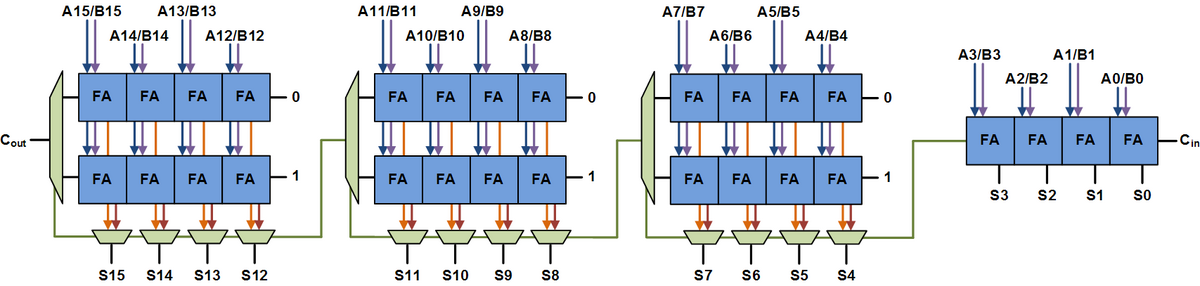
\includegraphics[width=\textwidth]{figs/EM-CSEA_linear.png}
    \caption{一个16比特线性进位选择加法器示意图}
\label{EM:Fig:CSEA_linear}
\end{figure}

图\ref{EM:Fig:CSEA_linear}展示了一个16比特线性CSEA的结构示意图,该加法器由一个4比特RCA和三个4比特CSEA组成,其关键路径包括初始的4比特RCA和后续三个MUX,可通过以下过程理解:当初始的RCA计算完成时,后面所有的小CSEA中的RCA均计算完成,只需等待真正的进位输入信号进行选择即可。
通常来讲,对于一个$n$比特线性CSEA,每个小CSEA的位宽取$\lfloor \sqrt n \rfloor$性能最好%
\IfStrEq{\Version}{Open}{%
    \footnote{\url{https://en.wikipedia.org/wiki/Carry-select_adder}},
}{,}
这里$\lfloor \ \rfloor$代表向下取整。

(2)平方根进位选择加法器

若级联的每个小CSEA的位宽不同,且数值大小从低位到高位依次为$2$、$3$、$4$、$\cdots$,初始RCA的位宽为2,则该可变大小CSEA被称为平方根CSEA,如图\ref{EM:Fig:CSEA_square}所示,关键路径为初始的2位宽的RCA和后续的3个MUX。
\begin{figure}[!htb]
    \centering
    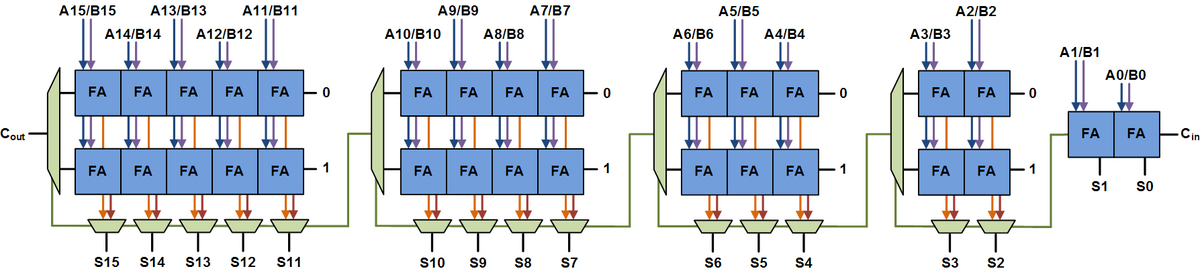
\includegraphics[width=\textwidth]{figs/EM-CSEA_square.png}
    \caption{16比特平方根进位选择加法器示意图}
\label{EM:Fig:CSEA_square}
\end{figure}
平方根CSEA假设全加器和MUX的延迟相等,避免了线性CSEA中高位CSEA计算完成后等待进位输入信号选择的缺点,不论位宽多大,其关键路径总是初始的2位宽RCA加上后续的MUX,与线性CSEA相比取得了显著的性能提升。不过,一般情况下全加器和MUX的延迟并不相等,因此需要根据实际情况决定使用哪种结构的CSEA。

\subsubsection{并行前缀加法器\cite{EM:book_Computer_Arithmetic}}

由式\eqref{EM:Eq:CLA}可得:
\begin{align}
    c_{i+1} = & \ \textcolor{blue}{g_i} +\textcolor{blue}{p_i} c_i \notag \\
          = & \ g_i + p_i \textcolor{red}{(g_{i-1} + p_{i-1} c_{i-1})} \notag \\
          = & \ \textcolor{blue}{(g_i + p_i g_{i-1})} + \textcolor{blue}{(p_i p_{i-1})} c_{i-1} \notag \\
          = & \ (g_i + p_i g_{i-1}) + (p_i p_{i-1}) \textcolor{red}{(g_{i-2} + p_{i-2} c_{i-2})} \notag \\
          = & \ \textcolor{blue}{(g_i + p_i g_{i-1} + p_i p_{i-1} g_{i-2})} + \textcolor{blue}{(p_i p_{i-1} p_{i-2})} c_{i-2} \notag \\
          = & \ \cdots
\label{EM:Eq:PPA_CLA}
\end{align}
设$i$、$j$均是整数且$0 \le i < j$,将$p$和$g$的定义从单比特拓展到连续的多比特,有:
\begin{align}
    & g_{[i,j]} =  g_j + p_j g_{j-1} + p_j p_{j-1} g_{j-2} + \cdots + (p_j p_{j-1} p_{j-2} \cdots p_{i+1}) g_i \notag \\
    & p_{[i,j]} = p_j p_{j-1} p_{j-2} \cdots p_i \notag \\
    & c_{j+1} = g_{[i,j]} + p_{[i,j]} c_i
\label{PPA_multi_bit_gp}
\end{align}
即对加法块$[i,j]$来讲同样存在进位的生成信号$g_{[i,j]}$和传播信号$p_{[i,j]}$,考虑到两者总是成对出现,可将其简写为二元对$(g_{[i,j]},p_{[i,j]})$。对两个相邻、部分重叠或完全重叠的加法块,$(g_{[i,j]},p_{[i,j]})$有如下性质:

相邻:假设$k$是整数且$i<k<j$,则块$[i,k-1]$与块$[k,j]$相邻,满足:
\begin{align}
    g_{[i,j]} = & \ g_{[k,j]} + g_{[i,k-1]} p_{[k,j]} \notag \\
    p_{[i,j]} = & \ p_{[i,k-1]} p_{[k,j]}
\label{EM:Eq:PPA_相邻}
\end{align}

部分重叠:假设$h$是整数且$i<k<h<j$,则块$[i,h]$与块$[k,j]$重叠,满足:
\begin{align}
    g_{[i,j]} = & \ g_{[k,j]} + g_{[i,h]} p_{[k,j]} \notag \\
    p_{[i,j]} = & \ p_{[i,h]} p_{[k,j]}
    \label{EM:Eq:PPA_部分重叠}
\end{align}

完全重叠,满足:
\begin{align}
    g_{[i,j]} = & \ g_{[i,j]} + g_{[i,j]} p_{[i,j]} \notag \\
    p_{[i,j]} = & \ p_{[i,j]} p_{[i,j]}
    \label{EM:Eq:PPA_完全重叠}
\end{align}

\begin{figure}[!b]
    \centering
    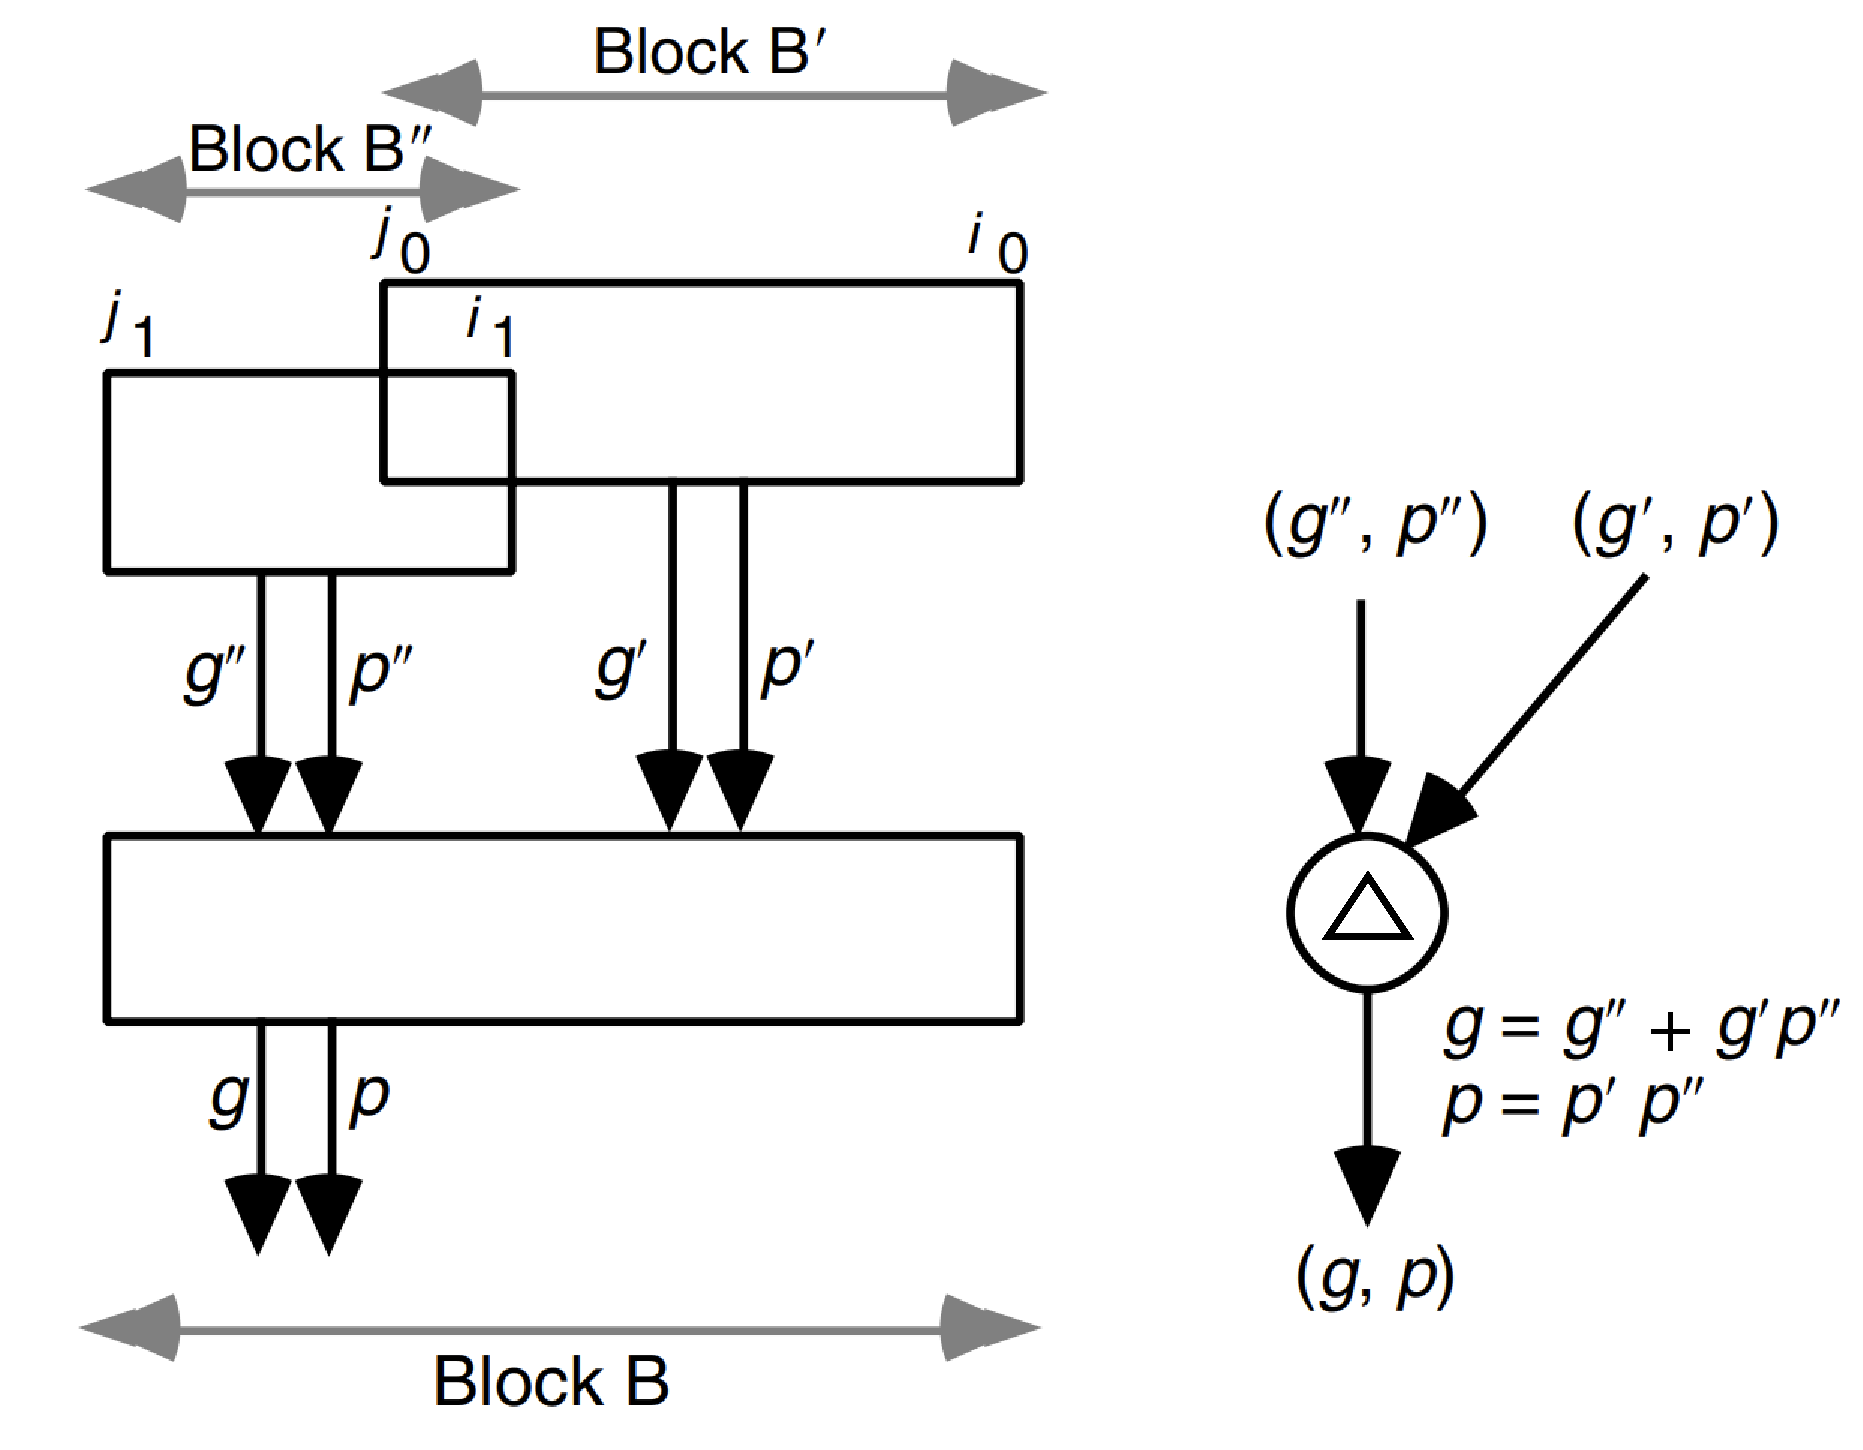
\includegraphics[width=0.6\textwidth]{figs/EM-PPA_BB.pdf}
    \caption{合并两个相邻或部分重叠的加法块$B \prime$、$B \prime \prime$的进位信号}
\label{EM:Fig:PPA_BB}
\end{figure}
如图\ref{EM:Fig:PPA_BB}所示,假设两个加法块$B \prime$和$B \prime \prime$相邻或重叠,则可以通过合并两对进位信号$(g \prime, p \prime)$和$(g \prime \prime, p \prime \prime)$来得到块$B$的进位信号$(g,p)$,假设该合并操作符号为$\triangle$,有:
\begin{equation}
    (g,p) = (g \prime, p \prime) \triangle (g \prime \prime, p \prime \prime)
\end{equation}
其中
\begin{equation}
    g = \ g \prime \prime + g \prime p \prime\prime , \ \ \ \ p = \ p \prime p \prime \prime
\end{equation}
注意$\triangle$满足结合律,不满足交换律:
\begin{align}
    ( \ (g \prime, p \prime) \triangle (g \prime \prime, p \prime \prime) \ ) \triangle (g \prime \prime \prime, p \prime \prime \prime) & \equiv (g \prime, p \prime) \triangle ( \ (g \prime \prime, p \prime \prime) \triangle (g \prime \prime \prime, p \prime \prime \prime) \ ) \notag \\
    (g \prime, p \prime) \triangle (g \prime \prime, p \prime \prime) & \not\equiv (g \prime \prime, p \prime \prime) \triangle (g \prime, p \prime)
\end{align}
这里假设块$B \prime \prime \prime$与块$B \prime \prime$相邻或重叠,进位信号为$(g \prime \prime \prime, p \prime \prime \prime)$。

基于此,可以定性地描述出进位问题:
假设加法器的位宽为$n$,给定$(g_0,p_0)$、$(g_1,p_1)$、$(g_2,p_2)$、$\cdots$、$(g_{n-1},p_{n-1})$,通过并行地计算
\begin{equation}
    (g_0,p_0) \triangle (g_1,p_1) \triangle (g_2,p_2) \triangle \cdots \triangle (g_{n-1},p_{n-1})
\end{equation}
能够得到所有的$(g_{[0,0]},p_{[0,0]})$、$(g_{[0,1]},p_{[0,1]})$、$(g_{[0,2]},p_{[0,2]})$、$\cdots$、$(g_{[0,n-1]},p_{[0,n-1]})$,即$c_1$、$c_2$、$c_3$、$\cdots$、$c_n$,且不同的并行方法对应不同的进位逻辑硬件实现,具有不同的面积和性能,称为并行前缀进位(Parallel Prefix Carry, PPC),得到的加法器被称为并行前缀加法器。
\begin{figure}[!htb]
    \centering
    \subfigure[超前进位加法器CLA的PPC树状图]{
    \label{EM:Fig:PPC_CLA}
    \begin{minipage}[t]{0.48\linewidth}
    \centering
    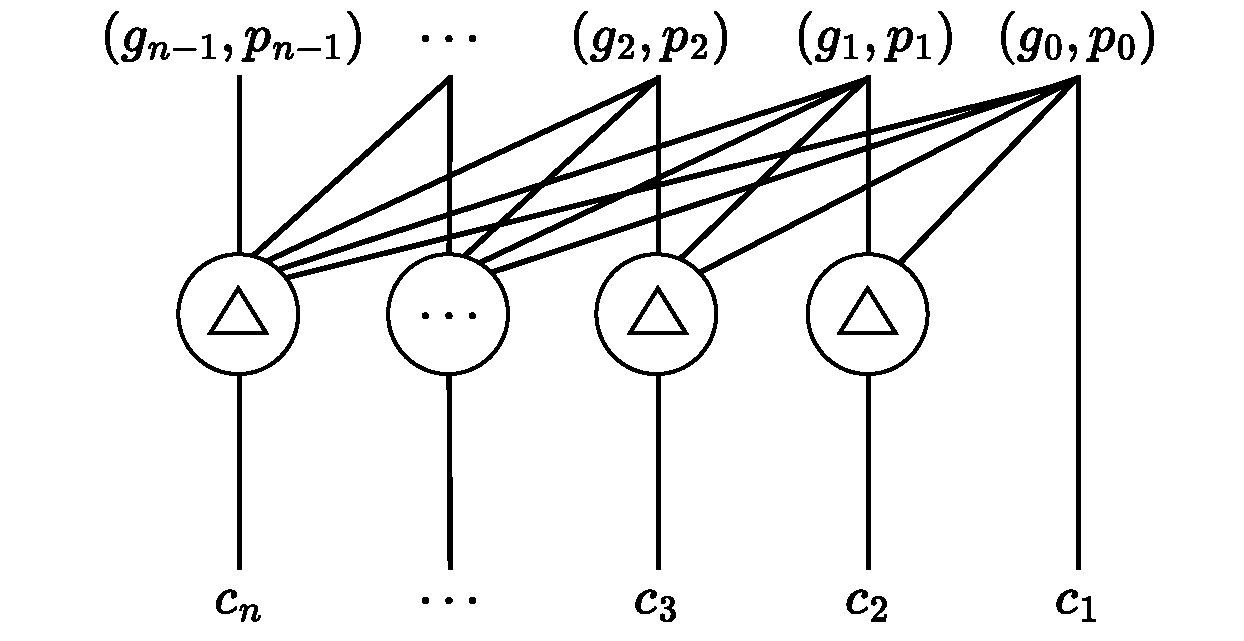
\includegraphics[width=\linewidth]{figs/EM-PPC_CLA.pdf}
    \end{minipage}
    }
    \subfigure[行波进位加法器RCA的PPC树状图]{
    \label{EM:Fig:PPC_RCA}
    \begin{minipage}[t]{0.48\linewidth}
    \centering
    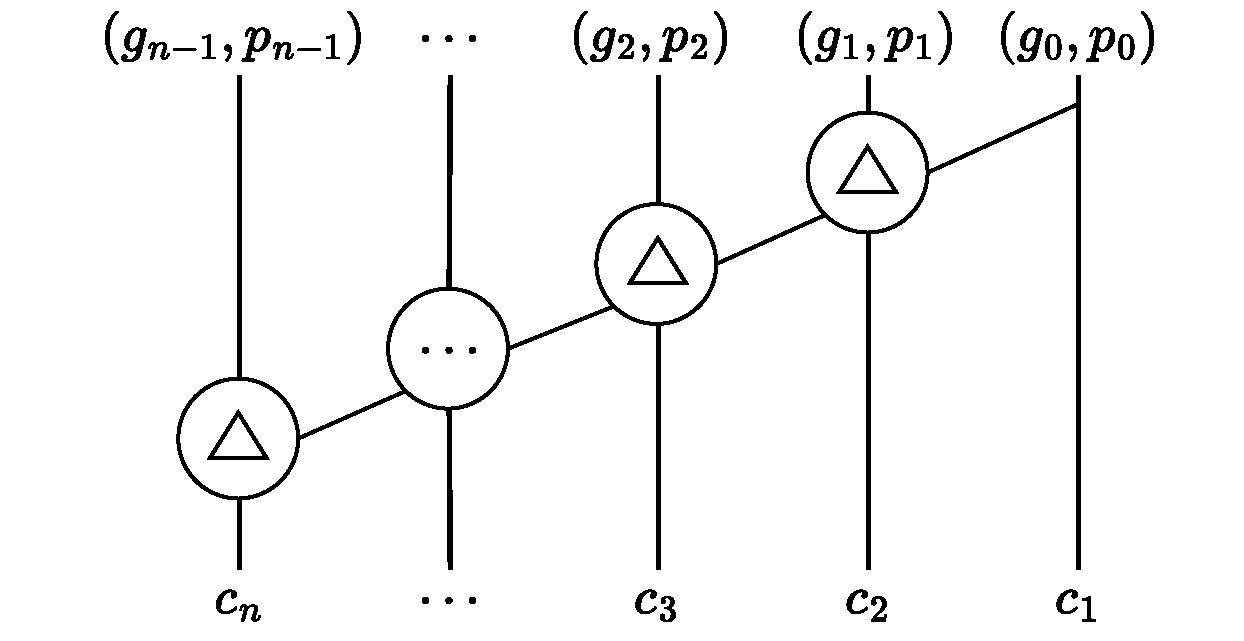
\includegraphics[width=\linewidth]{figs/EM-PPC_RCA.pdf}
    \end{minipage}
    }
\caption{标准CLA和标准RCA的PPC树状图}
\label{EM:Fig:PPC_CLA_RCA}
\end{figure}
PPC可由树状图进行表示,图\ref{EM:Fig:PPC_CLA_RCA}展示了标准超前进位加法器CLA和标准行波进位加法器RCA的PPC树状图。可以看到,CLA的PPC树状图只有一级,关键路径短,但计算量大;CLA的PPC树状图有$n$级,关键路径长,但使用了大量的中间节点,计算量小。因此,并行前缀加法器的核心在于如何对面积和延迟进行权衡,这为并行前缀加法器的设计带来了非常大的灵活性\cite{EM:PPA_PPT}:
比如1960年的Sklansky加法器\cite{EM:Sklansky_adder},特点是级数少、扇出高;
1973年的Kogge-Stone加法器\cite{EM:Kogge-Stone_adder},优点是逻辑级数和扇出都非常小,缺点是节点数量非常多,布线拥塞度高;
1980年的Ladner-Fisher加法器\cite{EM:Ladner-Fisher_adder},其结构与Sklansky加法器\cite{EM:Sklansky_adder}一致,原因是Ladner-Fischer形式化了进位问题的求解,Sklansky加法器是其中一种方案;
1982年的Brent-Kung加法器\cite{EM:Brent-Kung_adder},优点是扇出非常小,节点也较少,缺点是逻辑级数较多,即通过增加额外的逻辑级数来缓解扇出压力;
1987年的Han-Carlson加法器\cite{EM:Han-Carlson_adder},混合了Brent-Kung结构和Kogge-Stone结构,更有利于硬件实现;
1999年Knowles提出可以从逻辑深度、布线拥塞度和面积三个方面对进位网络的设计进行权衡\cite{EM:S-Knowles_adder};
2003年Harris提出了一个有趣的3-D结构图来对已有的并行前缀加法器进行分类\cite{EM:Harris_3-D},同时提出了一个新的进位结构;其余的前缀加法器包括Ling型加法器\cite{EM:Ling_adder}和具有多扇入节点的Beaumont-Smith加法器\cite{EM:Beaumont-Smith_adder}。
现代EDA(Electronic Design Automation)综合工具通常会根据用户的约束来实现具有不同并行前缀结构的加法器。由于大位宽下并行前缀网络的搜索空间巨大,英伟达利用强化学习的方法设计出了面积更小、速度更快的加法器\cite{EM:PrefixRL};也有工作在观察到EDA流程中逻辑综合和物理综合结果的不统一后\cite{EM:PPA_Pareto},通过图神经网络进行优化\cite{EM:PPA_GNN}。

\section{对数乘法器} \label{对数乘法器}

1962年,John N. Mitchell提出了一个相当有趣的算法\cite{EM:mitchell}:在二进制下,可以通过加法来近似得到两个无符号非零定点数的乘积,最大误差不超过$\dfrac{1}{9}$,且编程实现非常简洁,原理如下:

% 设$m=0$,由式\eqref{EM:Eq:unsigned_fixed_Decimal}得两个$n$比特二进制无符号正整数$X$和$Y$的十进制值:, 

对于式\eqref{EM:Eq:unsigned_fixed_Binary},假设$R=2$、$m=0$,两个$n$比特二进制无符号整数$X$和$Y$:
\begin{equation}
    X = x_{n-1} x_{n-2} x_{n-3} \cdots x_1 x_0 \ \ \ \ \ \ \ \
    Y = y_{n-1} y_{n-2} y_{n-3} \cdots y_1 y_0 
\label{EM:Eq:mitchell_XY_binary}
\end{equation}
若$X$和$Y$均非零(正整数),有:
\begin{align}
    x_{n-1} + x_{n-2} + x_{n-3} + \cdots + x_1 + x_0 = 1 \notag \\
    y_{n-1} + y_{n-2} + y_{n-3} + \cdots + y_1 + y_0 = 1
\end{align}
式中$+$表示逻辑或,则$X$和$Y$的十进制值为:
\begin{align}
    V(X) = \sum_{i=0}^{k_X} x_i 2^i \ \ \ \ \ \ \ \ \ \ \ \ \ \ \ 
    V(Y) = \sum_{i=0}^{k_Y} y_i 2^i
\end{align}
其中$k_X$和$k_Y$分别代表$X$和$Y$中最高位的1的权重值\cite{AC:AM:TOSAM},$X$和$Y$取不同值时$k_X$和$k_Y$的值也不同,乘积$P$的十进制值:
\begin{align}
    V(P) = & \ V(X)V(Y) \notag \\
    = & \ \sum_{i=0}^{k_X} x_i 2^i \times \sum_{i=0}^{k_Y} y_i 2^i \notag \\
    = & \ 2^{k_X} ( \ 1 + \sum_{i=0}^{k_X - 1} x_i 2^{i-k_X} \ ) \times 2^{k_Y} ( \ 1 + \sum_{i=0}^{k_Y - 1} y_i 2^{i-k_Y} \ ) \notag \\
    = & \ 2^{k_X + k_Y} ( \ 1 + \sum_{i=0}^{k_X - 1} x_i 2^{i-k_X} \ ) ( \ 1 +  \sum_{i=0}^{k_Y - 1} y_i 2^{i-k_Y}\ ) \notag \\
    = & \ 2^{k_X + k_Y} ( \ 1 + x^{\prime} \ ) ( \ 1 + y^{\prime} \ )
\label{EM:Eq:mitchell_P_orig}
\end{align}
其中
\begin{equation}
    x^{\prime} = \sum_{i=0}^{k_X - 1} x_i 2^{i-k_X} \ \ \ \ \ \ \ \
    y^{\prime} = \sum_{i=0}^{k_Y - 1} y_i 2^{i-k_Y}
\end{equation}
则:
\begin{equation}
    \log_2 (V(P)) = k_X + k_Y + \log_2 (1+x^{\prime}) + \log_2 (1+y^{\prime})
\label{EM:Eq:mitchell_log_P}
\end{equation}
易知$x, y \in [0,1)$,在这里,Mitchell做了一个相当果断而美妙的近似,那就是利用$\log_2 (1+x^{\prime}) \approx x^{\prime}$和$\log_2 (1+y^{\prime}) \approx y^{\prime}$将式\eqref{EM:Eq:mitchell_log_P}变为:
\begin{equation}
    \log_2 (V(P)) \approx k_X + k_Y + x^{\prime} + y^{\prime}
\label{EM:Eq:mitchell_log_P_2}
\end{equation}
则乘积$P$:
\begin{equation}
    V(P) \approx 2^{(k_X + k_Y)} \cdot 2^{(x^{\prime} + y^{\prime})}
\label{EM:Eq:mitchell_P_middle}
\end{equation}
这里再做一次近似:
\begin{equation}
    x^{\prime} + y^{\prime} \approx \left\{
    \begin{aligned}
        \ & \log_2 (1 + x^{\prime} + y^{\prime}) , & \ \ x^{\prime} + y^{\prime} < 1, \\
        \ & 1 + \log_2 (x^{\prime} + y^{\prime}), & \ \ x^{\prime} + y^{\prime} \ge 1.
    \end{aligned}
    \right.
\end{equation}
则式\eqref{EM:Eq:mitchell_P_middle}变为:
\begin{equation}
    V(P) \approx \left\{
    \begin{aligned}
        \ & 2^{(k_X + k_Y)} (1 + x^{\prime} + y^{\prime}) , & \ \ x^{\prime} + y^{\prime} < 1, \\
        \ & 2^{(k_X + k_Y + 1)} (x^{\prime} + y^{\prime}), & \ \ x^{\prime} + y^{\prime} \ge 1.
    \end{aligned}
    \right.
\label{EM:Eq:mitchell_P_final}
\end{equation}
式\eqref{EM:Eq:mitchell_P_final}即为Mitchell对数乘法器的最终形式,只需要加法、移位和检测电路即可完成两数相乘,可以证明Mitchell算法的最大误差不超过精确值的$\dfrac{1}{9}$。

在C++中,Mitchell算法有一个非常简单的实现%
\IfStrEq{\Version}{Open}{%
    \footnote{\url{https://kexue.fm/archives/7991}},
}{,}
单精度(Single precision)浮点数Mitchell算法的代码如算法\ref{EM:Alg:mitchell_Cpp}所示\cite{DNN:mitchell_Training},原理如下:

\begin{algorithm}[!]
    float int mitchell\_mul (const float a, const float b) \{ \\
    \ \ \ \ \ \ \ \ int c = *(int*)\&a + *(int*)\&b - 0x3f800000; \\
    \ \ \ \ \ \ \ \ return *(float*)\&c; \\
    \}
\caption{Mitchell算法在C++中的简单实现}
\label{EM:Alg:mitchell_Cpp}
\end{algorithm}

C++中int类型通常是32位,同时IEEE 754标准规定采用32个比特表示单精度浮点数,如图\ref{EM:Fig:mitchell_IEEE754}所示,其中最高位表示正负,之后8位表示科学计数法的指数,最后23位表示科学计数法的小数,注意指数部分需要加上偏移量127。对于两个单精度浮点数a和b,*(int*)\&a和*(int*)\&b其实就是把a和b对应的二进制表示拿出来,当作普通的int类型将两者相加,对应式\eqref{EM:Eq:mitchell_log_P_2},这时指数部分还多出一个偏移量,所以要减去这个偏移量,由于偏移量是127,并且后面还有23位,所以要减去常数$127×2^{23}$(十六进制为0x3f800000),最后将结果恢复成单精度浮点数。对双精度(Double precision)浮点数来说,在引入64比特位宽的long int类型和正确的偏移量($1023 \times 2^{52} = \text{0x3feffffb9f6e8000}$)之后,算法\ref{EM:Alg:mitchell_Cpp}同样适用(已验证)。

\begin{figure}[!htb]
    \centering
    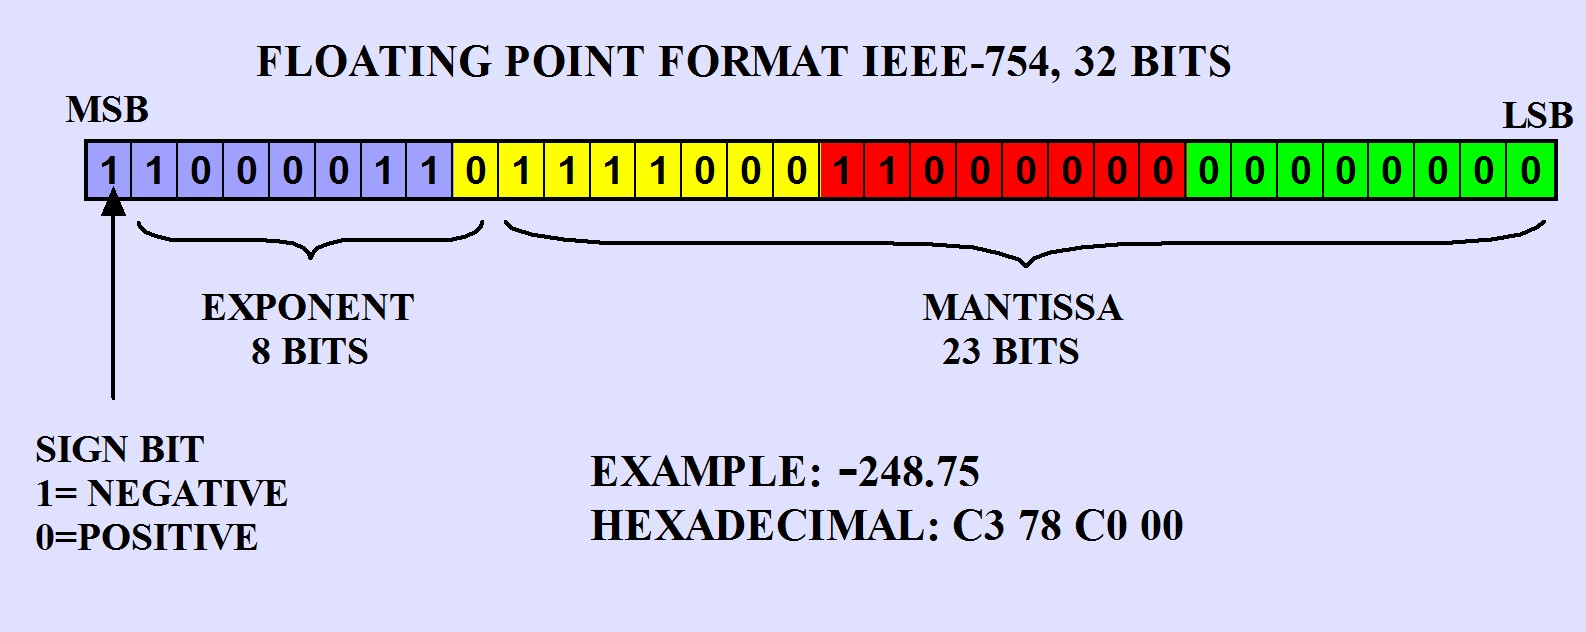
\includegraphics[width=0.8\linewidth]{figs/EM-mitchell_IEEE754.jpg}
    \caption{IEEE 754单精度浮点数标准}
    \label{EM:Fig:mitchell_IEEE754}
\end{figure}

Mitchell算法能够将乘法近似转化为加法实现,这对含有大量乘法并对误差有容忍性的神经网络应用带来了计算量优化的可能,比如文献\cite{DNN:mitchell_Training}在“ImageNet+ResNet50”中直接将神经网络中的精确乘法转换为Mitchell乘法,准确率只有轻微的下降,类似的工作也有多篇\cite{AC:AM:mitchell_aspdac2018,AC:AM:mitchell_tc2019}。

\section{近似电路的误差指标} \label{近似电路的误差指标}

近似电路通常是指近似的算术运算单元,如加法器、减法器、乘法器、除法器等。这些近似模块在计算中可能会产生误差,用来衡量误差的最基本的两个指标分别是误差率(Error Rate, ER)和误差距离(Error Distance, ED)\cite{AC:Arith:survey_hanjie}。ER表示产生错误结果的概率,ED代表近似结果和精确结果之间的算术差异。假设在某输入下近似电路的结果是$M \prime$,精确电路的结果是$M$,那么该输入下误差距离为:
\begin{equation}
    ED = | M′−M |
\label{AC:Arith:ED}
\end{equation}
相对误差距离(Relative ED, RED)表示近似结果与准确结果之间的相对算术差异,定义为:
\begin{equation}
    RED = \dfrac{ED}{M}
\label{AC:Arith:RED}
\end{equation}
ED和RED是衡量近似电路在某输入下误差的两个重要指标。

当考虑所有的输入情况时,可由平均误差距离(Mean ED, MED)和平均相对误差距离(Mean RED, MRED)来衡量近似电路和精确电路之间的整体算术差异,MED和MRED被定义为:
\begin{align}
    & MED = \sum _{i=1}^{N} ED_{i} \cdot P(ED_{i}) \label{AC:Arith:MED} \\
    & MRED = \sum _{i=1}^{N} RED_{i} \cdot P(RED_{i}) \label{AC:Arith:MRED}
\end{align}
其中$N$是所有输入情况的总数,$ED_{i}$和$RED_{i}$分别代表第$i$种输入情况下的误差距离ED和相对误差距离RED,$P(ED_{i})$和$P(RED_{i})$分别代表$ED_{i}$和$RED_{i}$发生的概率,即输入取第$i$种情况的概率。MED也被叫做平均绝对误差(Mean Absolute Error, MAE)。
归一化平均误差距离(Normalized MED, NMED)被定义为MED除以精确电路在所有可能输入情况下的最大值,常被用来比较同一近似设计方法在不同输入位宽下的误差表现。

均方误差(Mean Squared Error, MSE)和均方根误差(Root MSE, RMSE)也被广泛用于衡量近似电路和精确电路之间的整体算术差异,它们被定义为:
\begin{align}
    & MSE = \sum _{i=1}^{N}ED_{i}^{2}\cdot P(ED_{i}) \label{AC:Arith:MSE} \\
    & RMSE = \sqrt {MSE} \label{AC:Arith:RMSE}
\end{align}
另外,平均误差被定义为所有可能输入情况下$M \prime - M$的平均值,归一化平均误差被定义为平均误差除以精确电路在所有可能输入情况下的最大值。最后,最坏情况误差(Worst Case Error, WCE)反映了所有可能输入情况下ED的最大值。

以上提到的近似电路的误差指标均适用于近似乘法器。

\section{基于功能近似的近似乘法器相关工作}

从电路实现的底层结构上看,基于功能近似\cite{AC:ALS:survey}实现的近似乘法器设计方法可分为面向ASIC和FPGA两类,下面分别进行介绍。

\subsection{4类现有的ASIC近似乘法器设计方法}

(1)手工设计(Manual design)

手动化简乘法器的电路或门级网表的方法被称为手工设计方法,这种方法的优点在于通常能在不同位宽的乘法器之前迁移,缺点是费时费力,且无法灵活地根据应用的错误容忍程度进行调整,效果较差。

较为经典的一篇有关手工设计近似乘法器的工作是由Kulkarni等人\cite{AC:AM:KMap}于2011年发表的,他们观察到$2 \times 2$精确乘法器只有在输入是$3 \times 3$的时候才需要4个比特对输出进行表示,于是修改了卡诺图(Karnaugh map),将$3 \times 3 = 9$变为了$3 \times 3 = 7$,输出从原先需要4个比特减少到了3个比特,乘法器的门数降低了37.5\%,面积消耗更小。与精确的$2 \times 2$乘法器相比,该近似乘法器在16种可能的输入情况中,只有一种情况输出是错误的,误差率ER是$\dfrac{1}{16}$,由式\eqref{AC:Arith:ED}得输入为3$\times$3时的误差距离ED为$|7 − 9| = 2$。经过EDA软件评估,近似后的$2 \times 2$乘法器的面积相比精确版本减少了一半,并且拥有更短的关键路径。同时,由于近似后乘法器的开关电容更小,在相同工作频率下的动态功耗也更低。大位宽的乘法器可通过拆分的方法由近似的$2 \times 2$乘法器搭建起来,且搭建时可让高位输入保持精确乘法来降低误差。

文献\cite{AC:AM:CR}对行波进位加法器RCA中的全加器进行了重新设计,将进位输入信号替换成了前一级全加器的非进位输入,使进位链最多只能传播两位,优化了关键路径,降低了计算延迟,同时将截断进位链产生的误差保存了下来。优化后的全加器被排列成树形用于乘法器中部分积的累加及最终相加,并在最终相加后根据需要引入不同等级的误差补偿,提高乘法器的精度。精确的误差补偿需要考虑所有全加器保存的误差并相加,为了降低设计复杂度,仅考虑最高几位全加器保存的误差,通过或(OR)操作运算后加到最终的输出上。
图\ref{AC:AM:Fig:CR_app_adder}代表论文提出的考虑两级输入的近似全加器电路图,其中$S_i$和$E_i$分别代表求和输出与保存的误差。图\ref{AC:AM:Fig:CR_app_mul}展示了论文提出的基于近似全加器单元设计的近似乘法器的结构示意图,其中A1-A7代表树形的近似全加器阵列,一方面对部分积进行累加,一方面保留产生的误差,最后的补偿步骤选择最高4位全加器的结果进行运算。需要注意的是,因为保存的误差是通过或操作运算之后相加到结果上,所以即使考虑所有全加器保存的误差也无法将误差率降到0(正确的做法不是或运算而是相加)。
\begin{figure}[!htb]
    \centering
    \subfigure[考虑两级输入的近似全加器单元]{
    \label{AC:AM:Fig:CR_app_adder}
    \begin{minipage}[t]{0.3\linewidth}
    \centering
    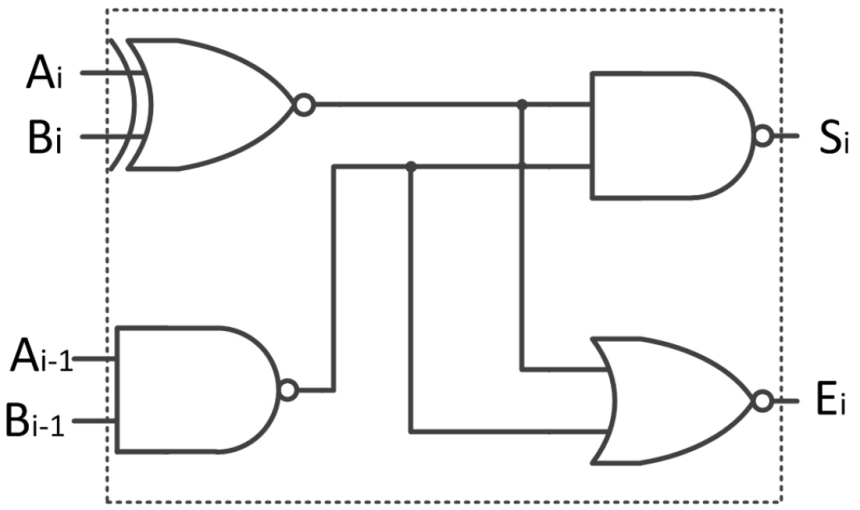
\includegraphics[width=\linewidth]{figs/AC-AM-CR_app_adder.png}
    \end{minipage}
    }
    \subfigure[提出的带有误差补偿模块的近似乘法器示意图]{
    \label{AC:AM:Fig:CR_app_mul}
    \begin{minipage}[t]{0.66\linewidth}
    \centering
    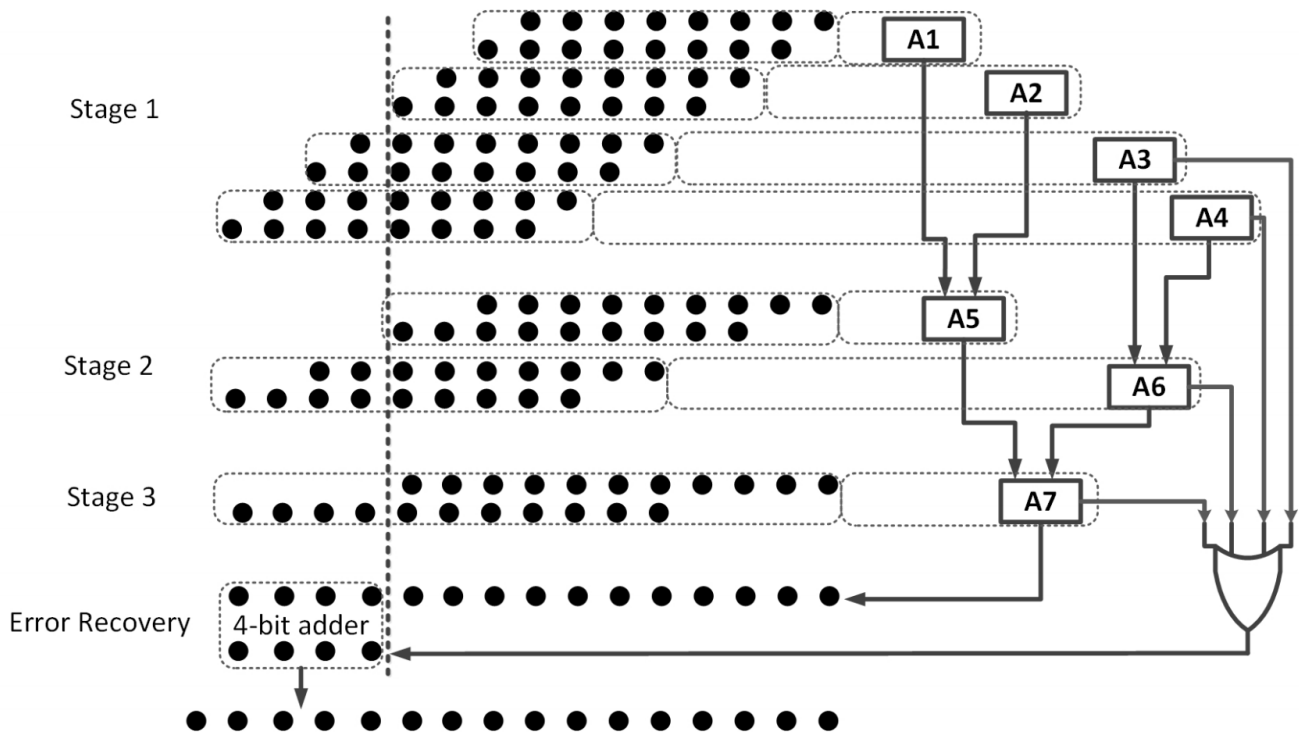
\includegraphics[width=\linewidth]{figs/AC-AM-CR_app_mul.png}
    \end{minipage}
    }
\caption{近似全加器单元和近似乘法器结构示意图}
\end{figure}

文献\cite{AC:AM:SDLC}在部分积生成后、累加前,先通过逻辑或(OR)操作有选择地对部分积进行了一次压缩,大大降低了部分积阵列的规模,减轻了后续的累加压力。除了2输入的或操作之外,更大输入的或操作也可以被使用,好处是部分积规模下降的更多,坏处是引入的误差更大。图\ref{AC:AM:Fig:SDLC_OR3}展示了利用3输入或门对部分积阵列进行压缩的过程:首先对部分积进行分组,每3个部分积一组,不足3个的可保持或使用更小输入的或门,同时避免操作高位部分积以减少误差,压缩后的部分积个数由8个减少为3个,降低了62.5\%。该论文提出的方法适用于不同位宽的乘法器,通过Synopsys Design Compiler综合工具对基于此方法设计的128比特位宽的近似乘法器进行评估发现,与精确乘法器相比,面积减少了45\%,关键路径减少了65\%。
\begin{figure}[!htb]
    \centering
    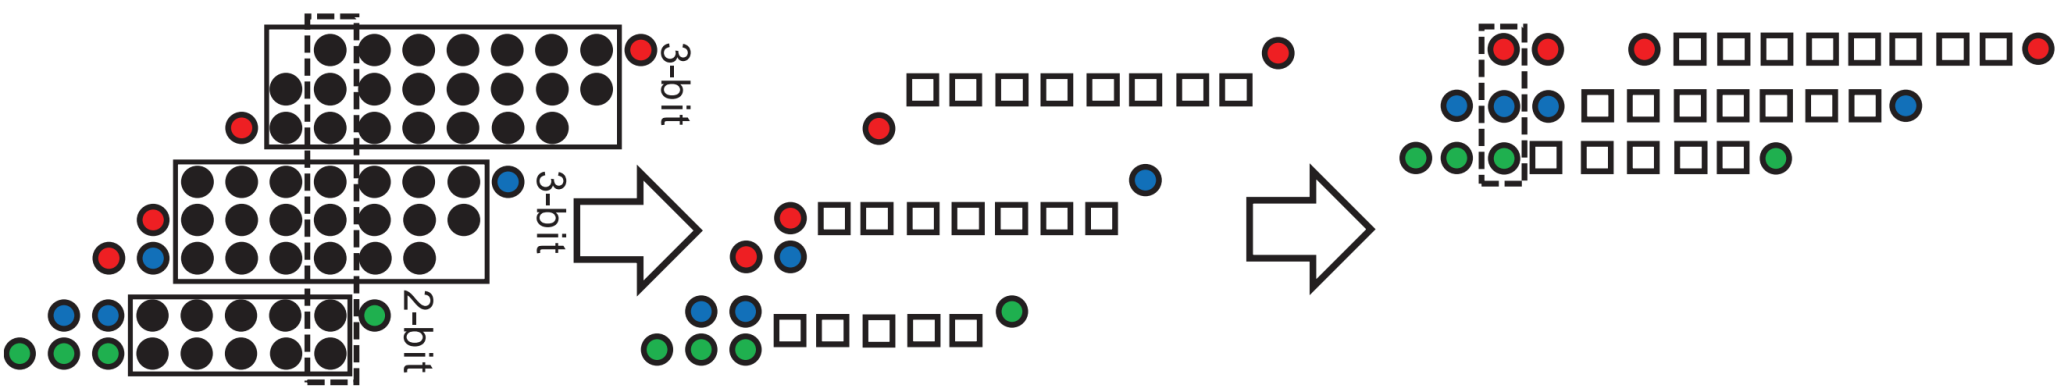
\includegraphics[width=\textwidth]{figs/AC-AM-SDLC_OR3.png}
    \caption{利用3输入或门对部分积阵列进行压缩}
\label{AC:AM:Fig:SDLC_OR3}
\end{figure}

文献\cite{AC:AM:DRUM}提出了一个用于两个无符号数相乘的动态无偏可配置乘法器DRUM,其基本思想是通过动态识别乘数和被乘数中权重最大的1的位置、挑选出以该位置开头的几个连续比特并对尾部数据进行四舍五入之后,利用一个小位宽的乘法器完成核心运算。整个电路包括检测器、四舍五入编码器、小位宽乘法器以及最后的移位器,可通过配置小乘法器的位宽来实现不同的精度。同时,该乘法器是无偏的,即平均误差为0(见\ref{近似电路的误差指标}有关平均误差的定义);该乘法器也是对称的,即对任意输入,交换乘数和被乘数后结果一致,没有极性。图\ref{AC:AM:Fig:DRUM_example}展示了DRUM计算过程的一个示例,在对操作数中挑出的部分比特四舍五入并执行乘法后,通过移位操作得到最终的结果。
\begin{figure}[!htb]
    \centering
    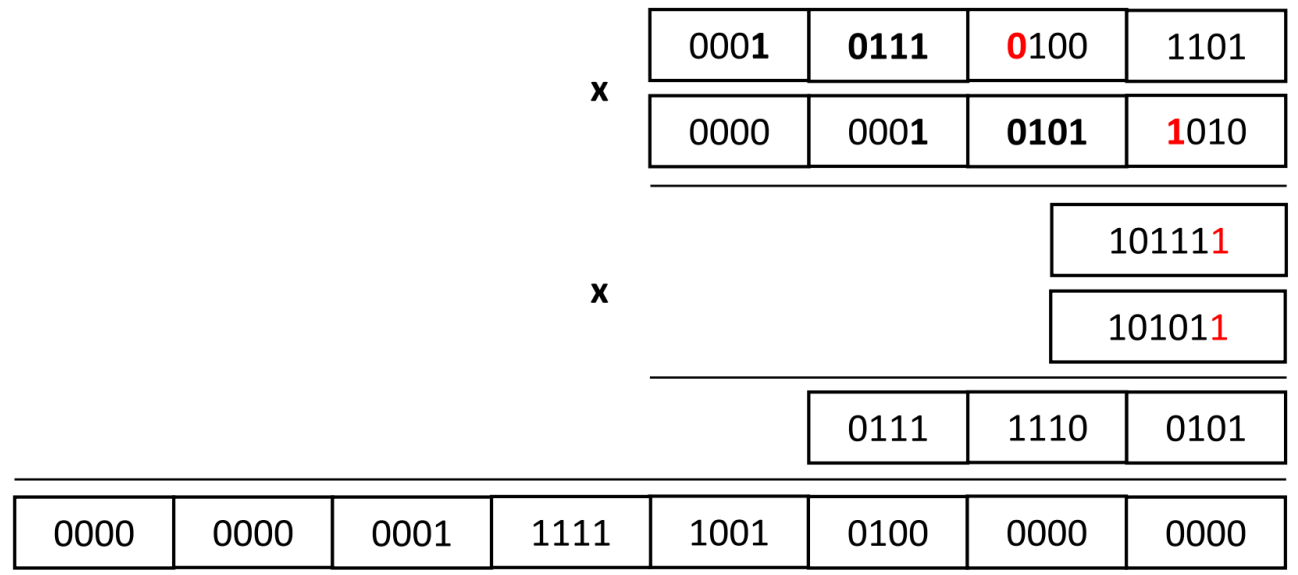
\includegraphics[width=0.7\textwidth]{figs/AC-AM-DRUM_example.png}
    \caption{DRUM计算过程的一个示例}
\label{AC:AM:Fig:DRUM_example}
\end{figure}

文献\cite{AC:AM:TOSAM}对式\eqref{EM:Eq:mitchell_P_orig}进行了变形:
\begin{align}
    V(P) = & \ 2^{k_X + k_Y} ( \ 1 + x^{\prime} \ ) ( \ 1 + y^{\prime} \ ) \notag \\
         = & \ 2^{k_X + k_Y} ( \ 1 + x^{\prime} \cdot y^{\prime} + x^{\prime} + y^{\prime} \ ) \notag \\
         \approx & \ 2^{k_X + k_Y} ( \ 1 + x^{\prime}_{App} y^{\prime}_{App} + x^{\prime}_T + y^{\prime}_T \ )
\label{AC:AM:Eq:TOSAM}
\end{align}
其中,$x^{\prime}_{App}$、$y^{\prime}_{App}$、$x^{\prime}_T$、$y^{\prime}_T$均是操作数中的部分比特,但与DRUM相比没有对尾部数据进行四舍五入而是直接丢弃,这样原始乘法被转换成了一个小位宽乘法和两个加法,减少了电路面积。同时,
$x^{\prime}_{App}$、$x^{\prime}_T$(或$y^{\prime}_{App}$、$y^{\prime}_T$)的位宽可以进行灵活地配置,能够满足不同应用的精度需求。

手工设计近似乘法器的方法众多,相当大一部分工作着重于对部分积的累加进行优化,这里只列举了几个比较典型和巧妙的示例,接下来介绍通过数学转换近似来实现近似乘法。

(2)数学转换近似(Mathematical transformation approximation)

数学转换近似通常需要问题满足一定的数学特性,通过将乘法转换为成本更低的操作来达到降低设计复杂度的目的,Mitchell提出的对数乘法器\cite{EM:mitchell}(见\ref{对数乘法器})可以看作是此方法的一个例子。乘法是一个非线性操作,文献\cite{AC:AM:OU}通过分段线性函数(Piece-wise linear function)来近似浮点数乘法中的尾数乘法器,原理如下:

假设近似乘法器基于线性基空间$\{1, x, y, x^2, y^2\}$实现,输入是$x$和$y$,范围分别是$[x_1,x_2]$和$[y_1,y_2]$($x_2 > x_1 \ge 0$,$y_2 > y_1 \ge 0$),则输出$z_{approx}$为:
\begin{equation}
    z_{approx} = k_0 + k_1 x + k_2 y + k_3 x^2 + k_4 y^2
\end{equation}
式中$k_0 \sim k_4$是待定常数。由\eqref{AC:Arith:ED}得误差距离ED的平方为:
\begin{equation}
    ED^2 = | \ z_{approx} - xy \ | ^2
\label{AC:AM:OU_ED2}
\end{equation}
通过最小化\eqref{AC:AM:OU_ED2}可以得到$k_0 \sim k_4$的解析解为:
\begin{equation}
    [k_{0}, k_{1}, k_{2}, k_{3}, k_{4}]=[-\frac{(x_{1}+x_{2})(y_{1}+y_{2})}{4},\frac{y_{1}+y_{2}}{2},\frac{x_{1}+x_{2}}{2}, 0,0]
\end{equation}
即将精确乘法转换为了线性操作:
\begin{equation} 
    xy \approx z_{approx} = k_{0}+k_{1}x+k_{2}y
\label{AC:AM:OU_AM}
\end{equation}
该近似乘法器在基空间$\{1, x, y, x^2, y^2\}$上误差距离ED的平方最小,且有以下几个性质:(a)对式\eqref{AC:AM:OU_AM}来说,当$\{x,y\}$取$\{x_1,y_1\}$、$\{x_1,y_2\}$、$\{x_2,y_1\}$、$\{x_2,y_2\}$时该近似乘法器的误差最大;(b)所得到的近似乘法器是无偏的,即平均误差为0:
\begin{equation} 
    \int\nolimits_{x_{1}}^{x_{2}}\int\nolimits_{y_{1}}^{y_{2}} ( \ k_{0}+k_{1}x+k_{2}y - xy \ ) \ dxdy = 0
\end{equation}
(c)若对精确乘法按照此论文提出的方法进行分段线性近似,即将输入范围$[x_1,x_2] \times [x_1,x_2]$划分为若干个子区域,在每个子区域内也将乘法转换成如式\eqref{AC:AM:OU_AM}所示的线性操作,则每个子区域面积相等时整个乘法器的误差距离ED的平方最小,且最小为:
\begin{equation}
    ED^2_\text{min} = \dfrac{ (x_2 - x_1)^3 (y_2 - y_1)^3 }{144 n^2}
\end{equation}
$n$是子区域的个数,因此可以通过不断划分面积相等的子区域来提高乘法器的精度。

对于浮点数来讲,尾数的取值范围为$[1,2)$,在不划分子区域的情况下,得到的近似乘法器为:
\begin{equation}
    z^0_{approx} = 1.5 x + 1.5 y - 2.25
\end{equation}
为了提高精度且方便硬件实现,对定义域进行划分,第$i$次划分后共生成$4^i$个子区域,每个子区域的面积相等。假设乘法器第$i$次划分后的输出比第$i-1$次划分后的输出差了$\Delta z^i_{approx}$,则:
\begin{equation}
    \Delta z^i_{approx} = z^i_{approx} -  z^{i-1}_{approx}
\end{equation}
经过证明,对任意的$i$,$\Delta z^i_{approx}$都可由一个异或XOR、一个移位、2个加法和几个反向逻辑实现,大大降低了误差补偿的成本,且第$i$次划分后乘法器的均方误差MSE为:
\begin{equation}
    MSE = \frac{1}{9\times 16^{i + 1}} \times \frac{1}{2^{23}}
\end{equation}
这里假设输入均匀分布。

\begin{figure}[!htb]
    \centering
    \subfigure[提出的近似浮点数乘法器架构图]{
    \label{AC:AM:Fig:OU_arch}
    \begin{minipage}[t]{0.53\linewidth}
    \centering
    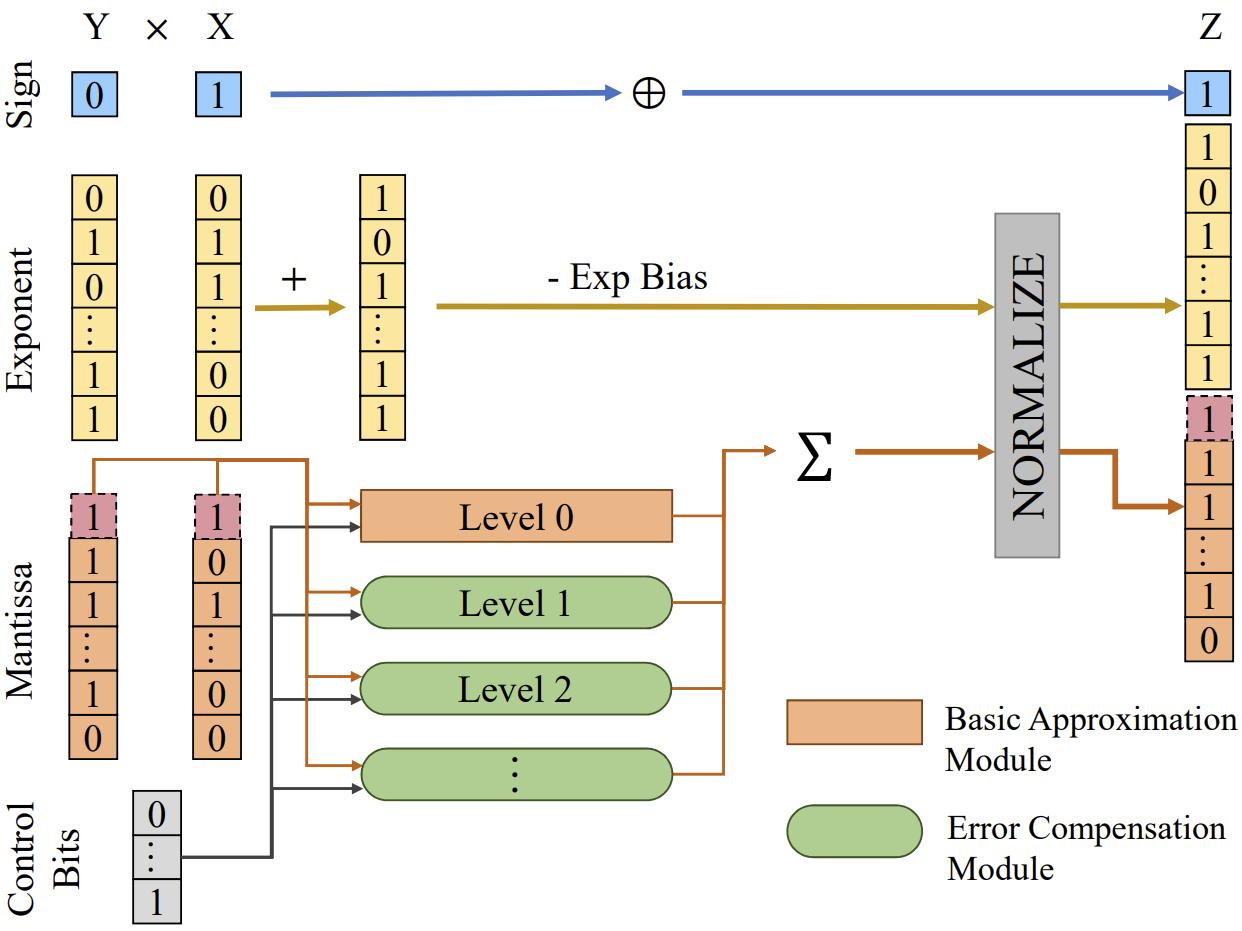
\includegraphics[width=\linewidth]{figs/AC-AM-OU_arch.png}
    \end{minipage}
    }
    \subfigure[不同划分等级下的误差分布图]{
    \label{AC:AM:Fig:OU_error}
    \begin{minipage}[t]{0.43\linewidth}
    \centering
    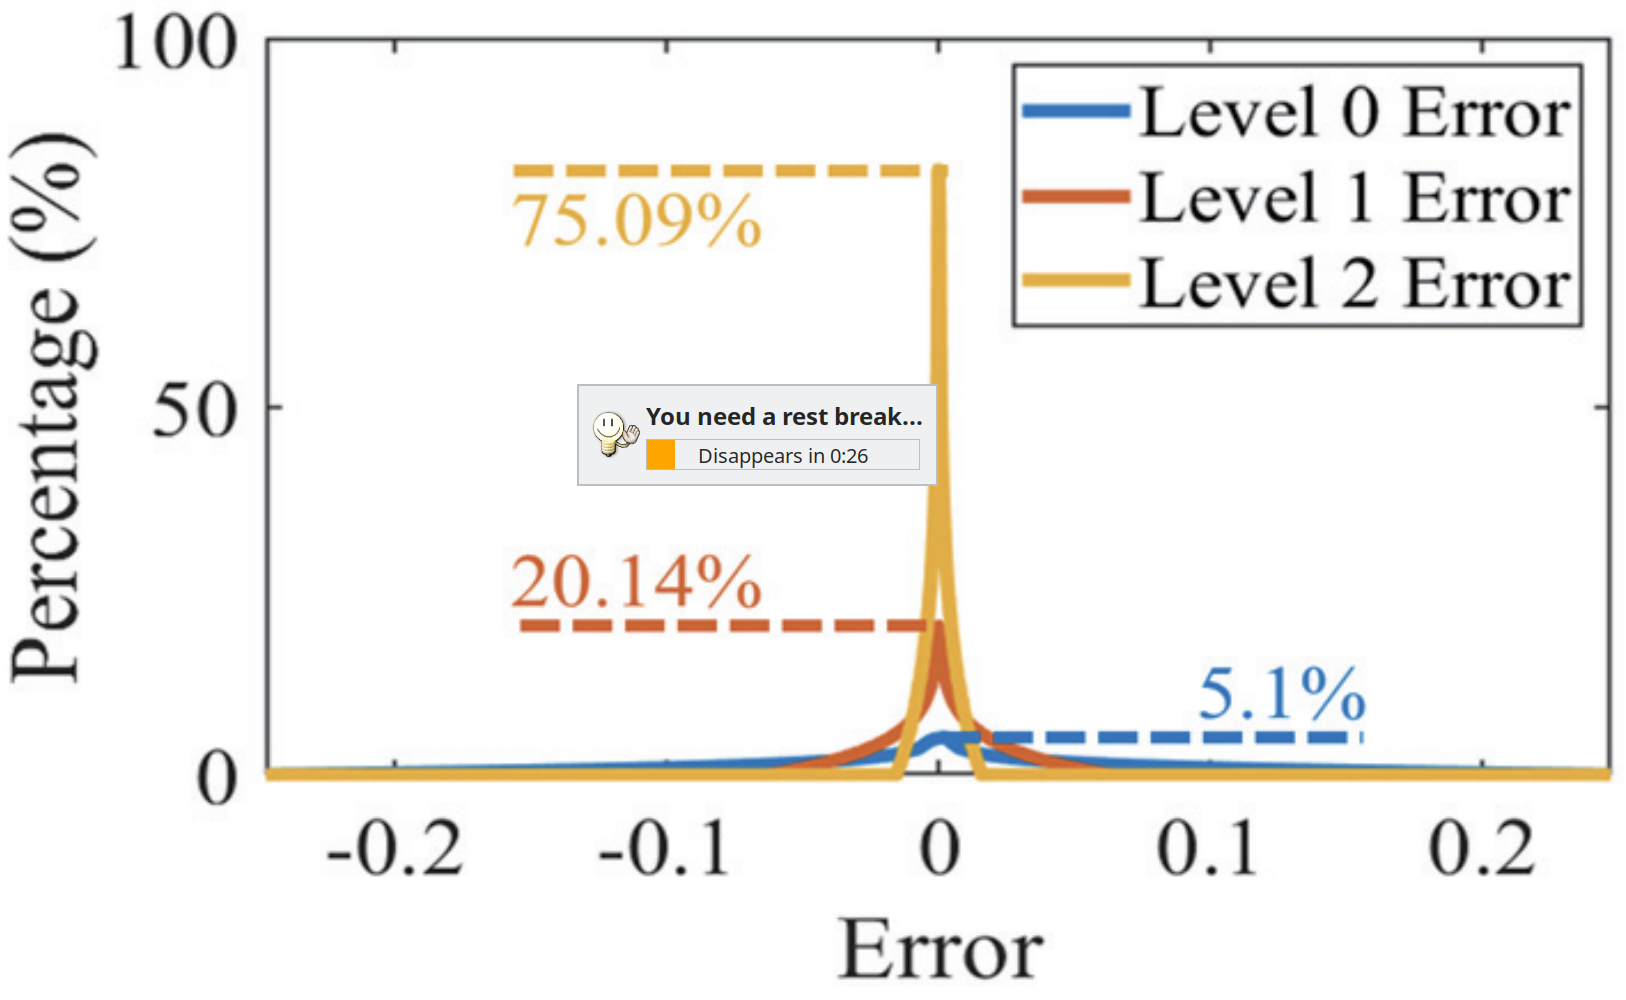
\includegraphics[width=\linewidth]{figs/AC-AM-OU_error.png}
    \end{minipage}
    }
\caption{论文所提出的近似浮点数乘法器架构图和不同划分等级下的误差分布}
\label{AC:AM:OU}
\end{figure}
图\ref{AC:AM:OU}展示了论文提出的近似浮点数乘法器的整体结构图和不同划分等级下的误差分布,可以看到随着划分次数的增加,误差在指数级减小。
尽管该方法是针对浮点数乘法器提出的,但经过简单的修改也可用于定点数乘法器。

(3)自动化方法(Automated method)

将设计近似乘法器的问题建模成搜索问题,能够利用计算机在短时间内生成大量具有不同精度和不同性能的近似乘法器。在自动化方法中,由捷克布尔诺理工大学(Brno University of Technology)可进化硬件(Evolvable HardWare, EHW)研究小组开发的、基于笛卡尔遗传规划(Cartesian Genetic Programming, CGP)\cite{CGP_2008,CGP_2011}的遗传算法(Genetic algorithm)取得了相当出色的效果。2016年,EHW的研究人员利用CGP设计了面向人工神经网络的近似乘法器\cite{AC:AM:CGP_2016},以精度下降小于2.80\%的代价节省了91\%的功耗。

CGP起源于Miller等人于1997年开发的一种进化数字电路的表示方法\cite{CGP_1997},在1999年第一次出现\cite{CGP_1999},其通用形式于2000年被正式提出\cite{CGP_2000}。
在CGP中,一个电路由一张有向无环图(Directed Acyclic Graph, DAG)进行表示,每个节点由一串整数组成,分别代表该节点从哪个节点获得数据以及节点对数据执行什么操作,输出没有被使用的节点可以被忽略。将所有的整数按照顺序排列,并在最后加上表示电路输出的节点编号便是电路对应的CGP形式。
\begin{figure}[!htb]
    \centering
    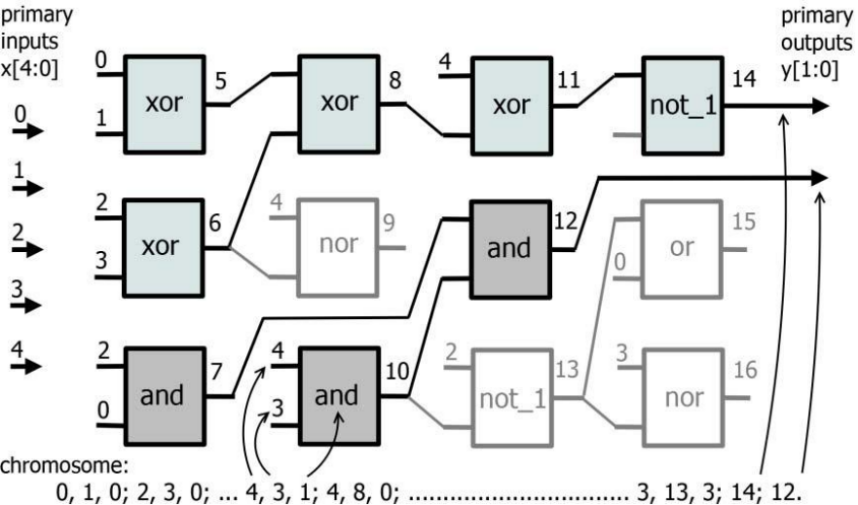
\includegraphics[width=0.8\linewidth]{figs/AC-AM-CGP.png}
    \caption{一个具有5比特输入、2比特输出的组合逻辑门级网表及其对应的CGP表示}
\label{AC:AM:CGP}
\end{figure}
图\ref{AC:AM:CGP}展示了一个具有5比特输入、2比特输出的组合逻辑门级网表及其对应的CGP表示,可以看到有4个门没有被使用。容易想到,若将一个精确乘法器的电路结构转换为CGP形式,那么改变CGP的表示形式便相当于改变了电路的功能,得到了近似乘法器。
Mrazek等人首先把8比特精确乘法器的不同电路实现结构转换成了CGP格式,然后随机改变CGP中的一部分整数得到近似乘法器,挑选出精度、延迟和功耗都较优的电路作为新的基础电路,不断迭代,在有限的时间内得到了均匀分布下误差较小、性能较高的471个近似乘法器,和430个近似加法器一起组成了一个开源的近似算术单元库EvoApprox8b\cite{AC:AM:CGP_Evoapprox8b}。考虑到许多应用中乘法器的输入数据分布并不是均匀的,在修改遗传算法中的目标函数后,CGP也可以被用于生成面向特定分布的高质量近似乘法器\cite{AC:AM:CGP_2019}。
如果乘法器的位宽较大,CGP等自动化方法生成的近似乘法器往往无法快速得到误差的边界,文献\cite{AC:AM:CGP_32bit}将近似等价性检查的形式化技术集成到CGP的搜索中,能够将搜索推向可快速验证的近似电路,方法通过ABC\cite{LS:ABC}工具实现,并对最大32比特位宽的乘法器进行了评估,结果显示提出的方法在几小时内生成了一组高质量的32位近似乘法器。

(4)近似电路综合(Approximate circuit synthesis)

近似电路综合(Approximate Circuit Synthesis)\cite{AC:ALS:survey}是近似逻辑综合的一个细分方向,着重于近似算术单元的生成,属于近似电路设计方法中功能近似(见\ref{approximate_computing_advance}有关功能近似的定义)的一种。
给定一个精确电路的描述和约束(通常是误差),近似电路综合不需要知道具体的电路功能,自动化生成满足精度的电路实现,与自动化方法相比,近似电路综合可直接应用于各种算术单元,通用性更强。近似电路综合可以通过网表转换(Netlist transformation)或布尔重写(Boolean rewriting)的方式实现,
\begin{figure}[!htb]
    \centering
    \subfigure[网表转换方法实现近似电路,左:精确电路的门级网表,右:生成的近似电路的门级网表]{
    \label{AC:ALS:survey_net_trans}
    \begin{minipage}[t]{\linewidth}
    \centering
    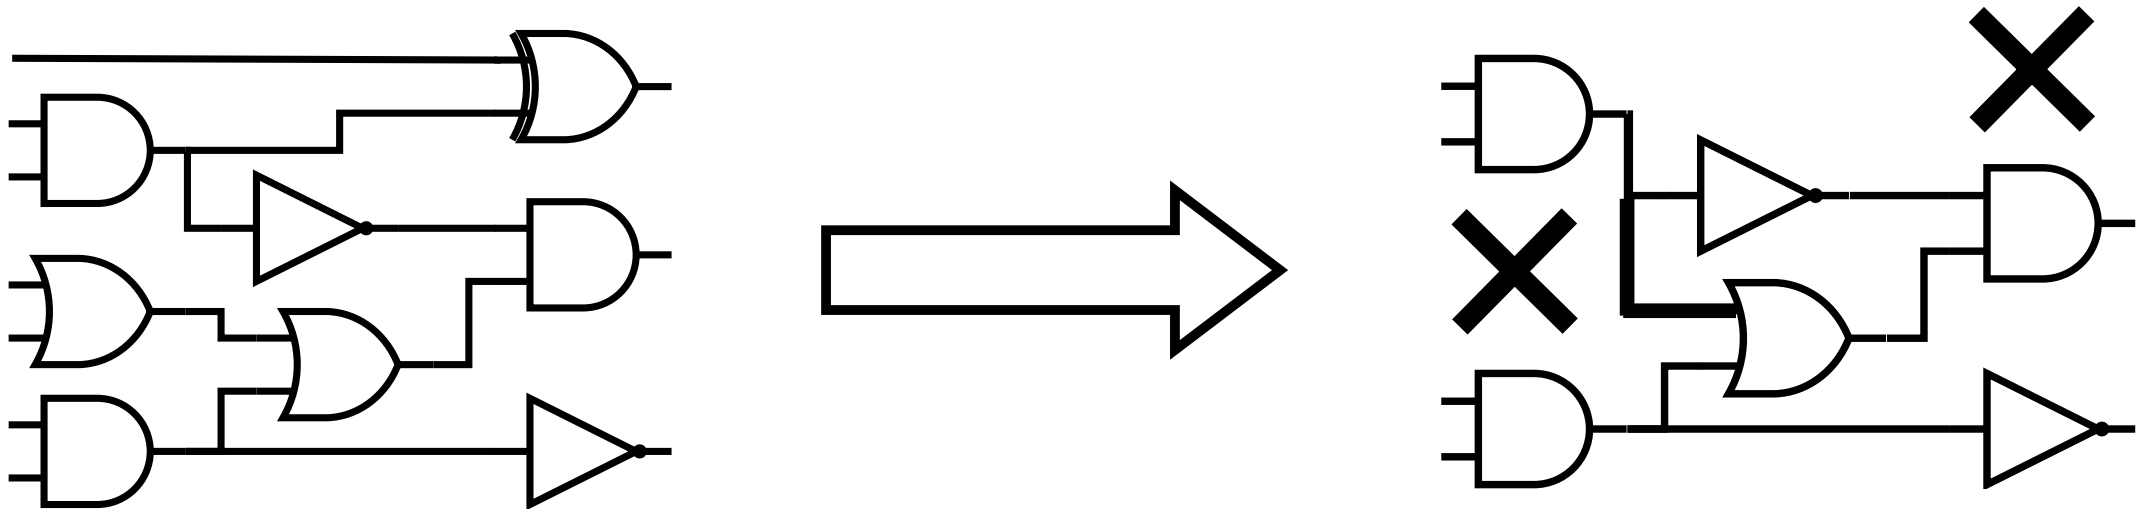
\includegraphics[width=0.8\linewidth]{figs/AC-ALS-survey_net_trans.png}
    \end{minipage}
    }
    \subfigure[布尔重写方法实现近似电路,左:精确电路的真值表,右:生成的近似电路的真值表]{
    \label{AC:ALS:survey_bool_rewr}
    \begin{minipage}[t]{\linewidth}
    \centering
    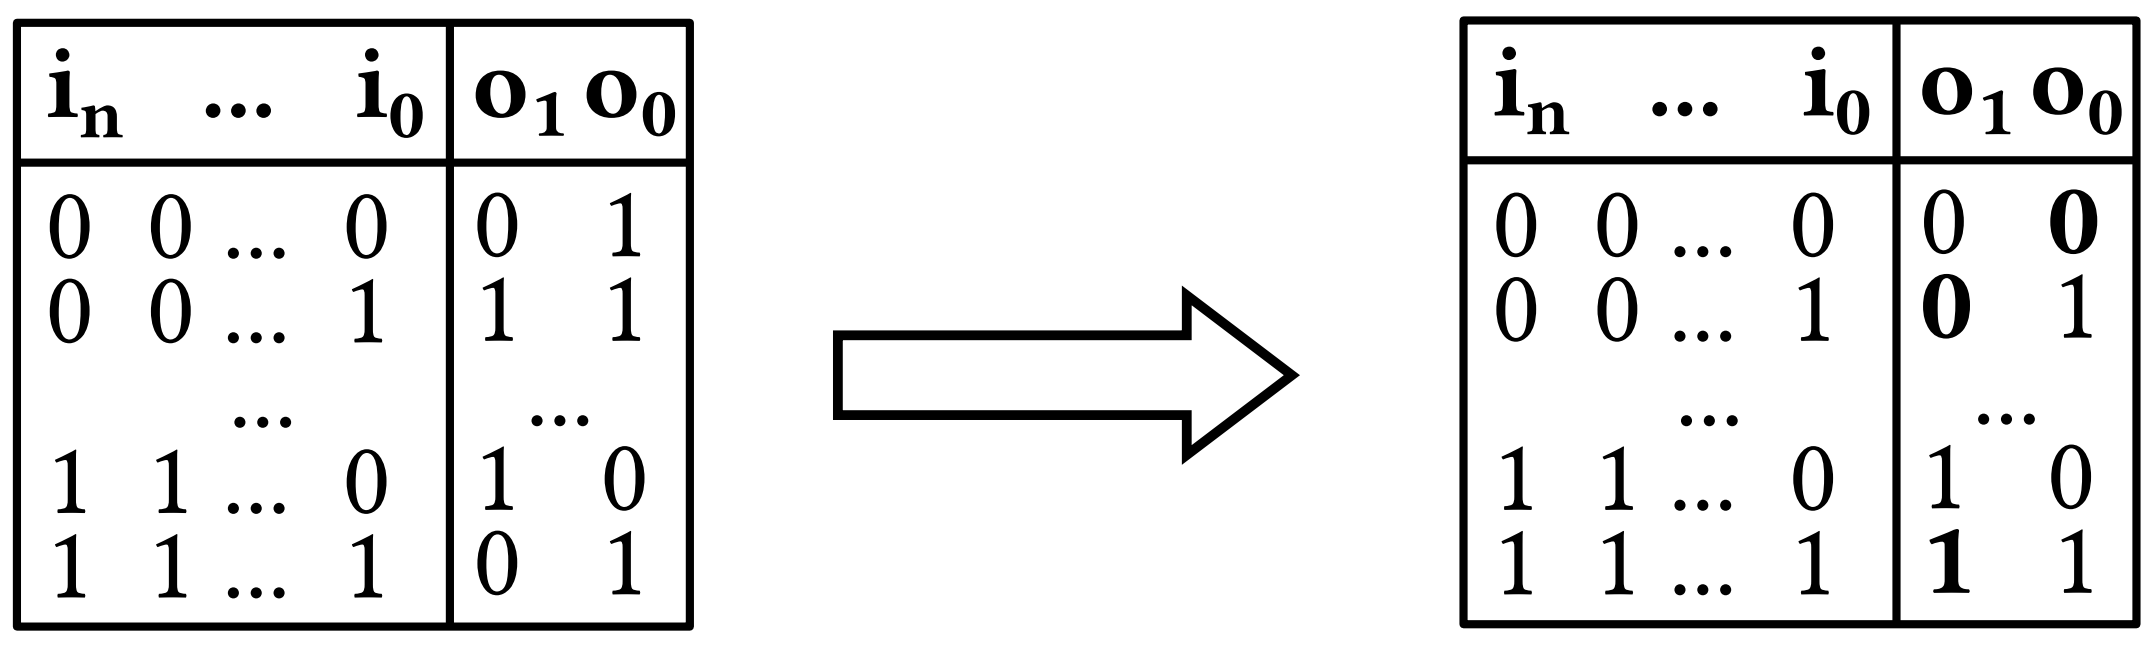
\includegraphics[width=0.75\linewidth]{figs/AC-ALS-survey_bool_rewr.png}
    \end{minipage}
    }
\caption{实现近似电路综合的两种常见方式}
\label{AC:ALS:survey_ACS_two_methods}
\end{figure}
图\ref{AC:ALS:survey_ACS_two_methods}举例展示了两种实现方式的区别,具体来讲,网表转换方式通过移除一些逻辑节点或用导线直接替换节点来对精确电路的门级网表进行简化,以达到减小面积和降低功耗的目的,而布尔重写方式则着重于修改抽象级别更高的真值表,使对应的布尔表达式更简洁紧凑。

文献\cite{AC:ALS:ALSRAC}采用网表转换的方法,利用重替换(resubstitution)算法\cite{LS:resub}不断尝试修改电路的局部结构,每次修改后用仿真的方式确定误差,直到找到满足精度要求的电路后退出。该方法被Meng等人基于ABC\cite{LS:ABC}实现并命名为ALSRAC,实验结果表明,ALSRAC产生的近似电路的面积与国际前沿工作相比减小了7\%-18\%。


\subsection{基于查找表编码的FPGA近似乘法器}

在介绍有关FPGA近似乘法器的工作之前,对FPGA的结构及乘法实现原理做一个介绍是必要的。
在FPGA中,算术操作通常由DSP模块实现,但DSP电路的面积只占整个FPGA芯片的5\%,且位置固定\cite{FPGA:DSP},这意味着某些需要大量乘法的应用比如DNN无法在FPGA上被有效的映射\cite{FPGA:Math}。相对应的,FPGA中存在着丰富的查找表单元,能够和布线资源一起实现复杂的函数功能,某些充分考虑LUT特性的设计能够在FPGA上实现相当高的性能\cite{FPGA:PolyLUT}。
然而,一块FPGA芯片的容量是有限的,对于大型设计来讲往往需要将其划分后部署到不同的FPGA芯片上,这会极大地降低电路的性能。同时FPGA中的布线资源昂贵,如果查找表单元使用的过多,有可能会造成布线拥塞,也会对电路的性能造成影响。
所以有必要在FPGA中使用近似乘法器来提高乘法的效率,降低FPGA资源的使用量,提高电路的性能。

\begin{figure}[!h]
    \centering
    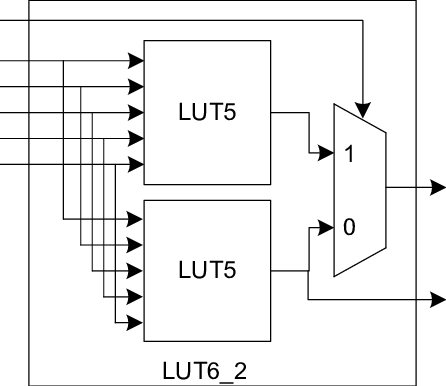
\includegraphics[width=0.5\linewidth]{figs/FPGA-LUT6_2.png}
    \caption{一个典型的拥有6个输入的LUT结构图}
    \label{FPGA:Fig:LUT6_2}
\end{figure}

LUT通常由多路选择器MUX和SRAM构成,其大小可根据输入个数的不同进行区分,一个$n$输入的LUT包含$2^n -1$个MUX和$2^n$个SRAM,能实现任意的$n$输入函数(共$2^{2^n}$个),可看作两个$n-1$的输入LUT和一个二选一MUX的组合。
目前最常用的LUT的输入个数为6\cite{FPGA:VIB},简称为LUT6。图\ref{FPGA:Fig:LUT6_2}展示了一个由两个LUT5组成的LUT6示意图,被称为LUT6\_2。LUT6\_2共包含$64$个SRAM,在编码后每个SRAM都有一个确定的值,被称为初始(Initial, INIT)值,不同INIT值的组合能够实现不同的函数,一共有$2^{64}$种组合,能够实现任意的6输入函数。

\begin{figure}[!h]
    \centering
    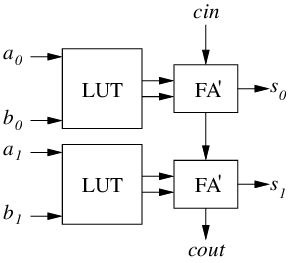
\includegraphics[width=0.4\linewidth]{figs/FPGA-carry_chain.png}
    \caption{一种2比特位宽的FPGA进位链结构示意图}
    \label{FPGA:Fig:carry_chain}
\end{figure}

虽然LUT能够实现特定输入数下的任意单输出函数,但对多输入多输出的算术操作的运算效率并不高。
考虑到加法使用最频繁,为了提高性能,FPGA引入了进位链来降低加法的进位延迟,
一种典型的2比特位宽的进位链结构如图\ref{FPGA:Fig:carry_chain}所示,由两个进位单元级联而成,每个进位单元包含一个LUT和一个伪全加器FA$'$,每个LUT的结构如图\ref{FPGA:Fig:LUT6_2}中的LUT6\_2所示。
根据式\eqref{EM:Eq:CLA}得全加器的进位信号:$c_{i+1} = p_i c_i  + \overline{p_i} g_i$,求和信号:$s_{i} = p_i \oplus g_i$,则可利用LUT6\_2中的两个LUT5产生进位的传播信号和生成信号送给伪全加器FA$'$,伪全加器FA$'$通过一个异或门XOR和一个二选一MUX进行求和及进位输出,MUX可由延迟较低的传输管结构实现。通过级联更多的进位单元可实现更大位宽的进位链。

文献\cite{AC:AM:FPGA:SMApproxLib}通过手动修改精确乘法器中用于部分积累加的LUT的INIT值,设计了几个拥有不同误差和不同硬件成本的近似乘法器,提出并开源了第一个面向FPGA领域的近似乘法器库SMApproxLib。类似地,文献\cite{AC:AM:FPGA:CaCc,AC:AM:FPGA:FPT22,AC:AM:FPGA:TCAD22}也采用了修改精确模式下LUT中SRAM编码的方法来得到误差不同的近似乘法器。



\section{逻辑综合介绍}


\subsection{Yosys和ABC}

\begin{figure}[!htbp]
    \centering
    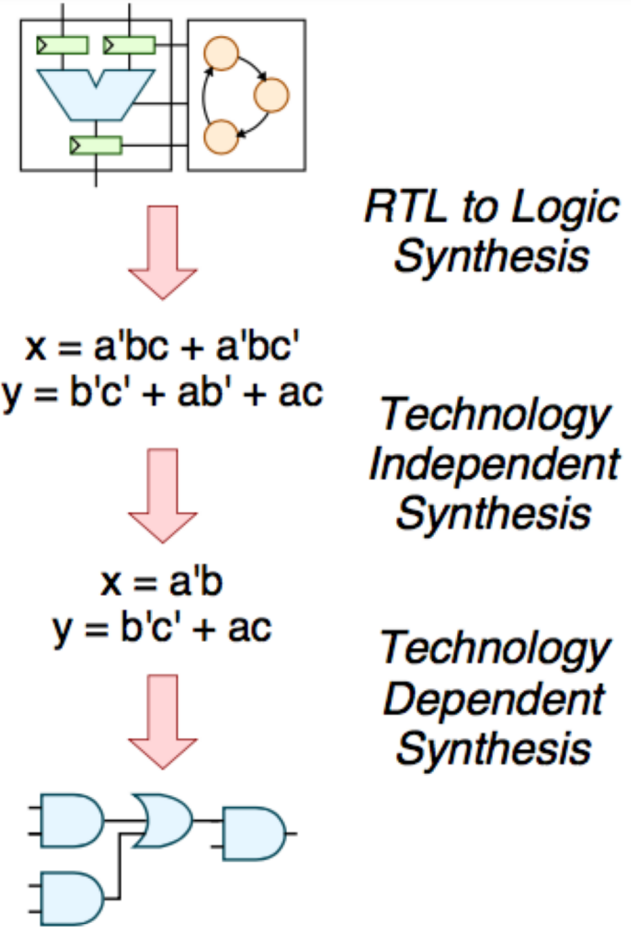
\includegraphics[width=0.4\linewidth]{./figs/LS-flow.png}
    \caption{传统逻辑综合流程图}
    \label{LS:flow}
\end{figure}

\begin{figure}[!htbp]
    \centering
    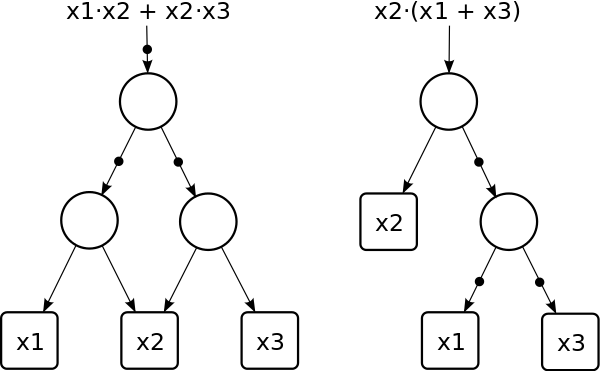
\includegraphics[width=0.6\linewidth]{./figs/LS-two_AIG.png}
    \caption{函数$x_2 (x_1 + x_3)$的两种不同的AIG实现}
    \label{LS:two_AIG}
\end{figure}


图\ref{LS:flow}展示了传统逻辑综合的流程图,首先将用户设计的寄存器传输级电路读入并解析,然后进行一系列工艺无关的逻辑优化操作,最后进行工艺相关的映射,生成门级网表。在现代EDA工具中,解析后电路中的组合逻辑部分通常由一个有向无环图进行表示,被称为布尔网络\cite{FPGA:CLB_Anderson},网络中的节点代表逻辑函数,边代表连接关系,逻辑综合进行的一系列优化及映射操作都基于该网络实现。
在一个布尔网络中\cite{LS:exact_rewriting,FPGA:Jason_Cong_1993,LS:Verification_after_synthesis},一个节点的扇入(Fanin)和扇出(Fanout)分别指该节点的输入节点和输出节点;
假设存在一条路径从节点$v$到节点$w$,则$v$是$w$的传递扇入(Transitive fanin),$w$是$v$的传递扇出(Transitive fanout);
网络的主要输入(Primary Inputs, PIs)是指所有的无扇入节点,网络的主要输出(Primary Outputs, POs)是指所有与外部相连的节点;
一条路径的长度指经过的节点数目;
节点的深度或级数指从网络的所有主要输入到该节点的所有路径中最长路径的长度;
最大节点深度被称为网络的深度。

% 图\ref{LS:boolean_net}展示了一个简单的布尔网络的示意图,可以看作是有5个输入、6个输出、7个节点、16条边的DAG,

% \begin{figure}[!htbp]
%     \centering
%     \includegraphics[width=0.8\linewidth]{./figs/LS-boolean_net.png}
%     \caption{一个简单的布尔网络示意图}
%     \label{LS:boolean_net}
% \end{figure}

AIG(And-Inverter Graph)是目前一种被广泛用来对逻辑函数进行表示和优化的有向无环图\cite{LS:AIG},在AIG中,节点分为主要输入节点、主要输出节点和2输入的与门节点三种类型,边包括取反和不取反两种情况,主要输入节点没有输入边,主要输出节点可能有输出边。一个逻辑函数可由不同结构的AIG表示,图\ref{LS:two_AIG}展示了函数$x_2 (x_1 + x_3)$两种不同的AIG实现。基于AIG,由Berkeley大学研发的的逻辑综合与验证工具ABC\cite{LS:ABC}在学术界和工业界获得了广泛的关注和赞誉。ABC可以对AIG进行逻辑优化和工艺映射,逻辑优化的目标是最小化AIG的规模和深度,映射目标是最小化LUT或ASIC电路的面积和延迟。


% 研究表明\cite{LS:structural_bias},AIG的映射结果会受到结构偏差(Structural bias)问题的影响,具体来说,同一个AIG进行不同的变换后会有不同的映射结果,且质量差别较大,这是由于AIG结构的不同导致映射器无法发现更优的解。图\ref{LS:structural_bias}展示了结构偏差问题的存在对LUT映射质量产生影响的一个示例,

% \begin{figure}[!htbp]
%     \centering
%     \includegraphics[width=\linewidth]{./figs/LS-structural_bias.png}
%     \caption{结构偏差问题影响LUT映射质量的一个示例}
%     \label{LS:structural_bias}
% \end{figure}


在逻辑优化阶段,ABC存在着许多不同的命令对AIG进行变换和化简,典型的命令包括balance, refactor, rewrite等,不同的优化命令会对AIG产生不同的优化效果,开发人员根据经验预先设定了一些优化脚本(如resyn2)对不同的电路进行使用。然而,不同命令的组合及顺序对逻辑优化的效果有很大影响,并且当优化进行到一定程度后,继续优化并不一定会对后续的映射操作起到正面效果\cite{LS:PIMap},因此必须针对不同的电路提供不同的优化序列,以达到对不同电路都能实现良好提升的目的。为给定的布尔逻辑网络寻找较优逻辑优化命令组合的问题被称为序列探索。

ABC能够利用AIG对布尔网络进行有效地表示和变换,但在电路解析方面能力不足。目前使用最广泛的硬件描述语言(Hardware description language)是Verilog-2005,被大多数EDA工具支持。Yosys\cite{LS:yosys}是一款开源的Verilog解析工具,支持绝大部分Verilog-2005语法,与ABC结合能够完成从Verilog到门级网表的全流程工作。

\subsection{用来表示布尔网络的不同DAG形式}

(1)XAIG

\begin{figure}[!htbp]
    \centering
    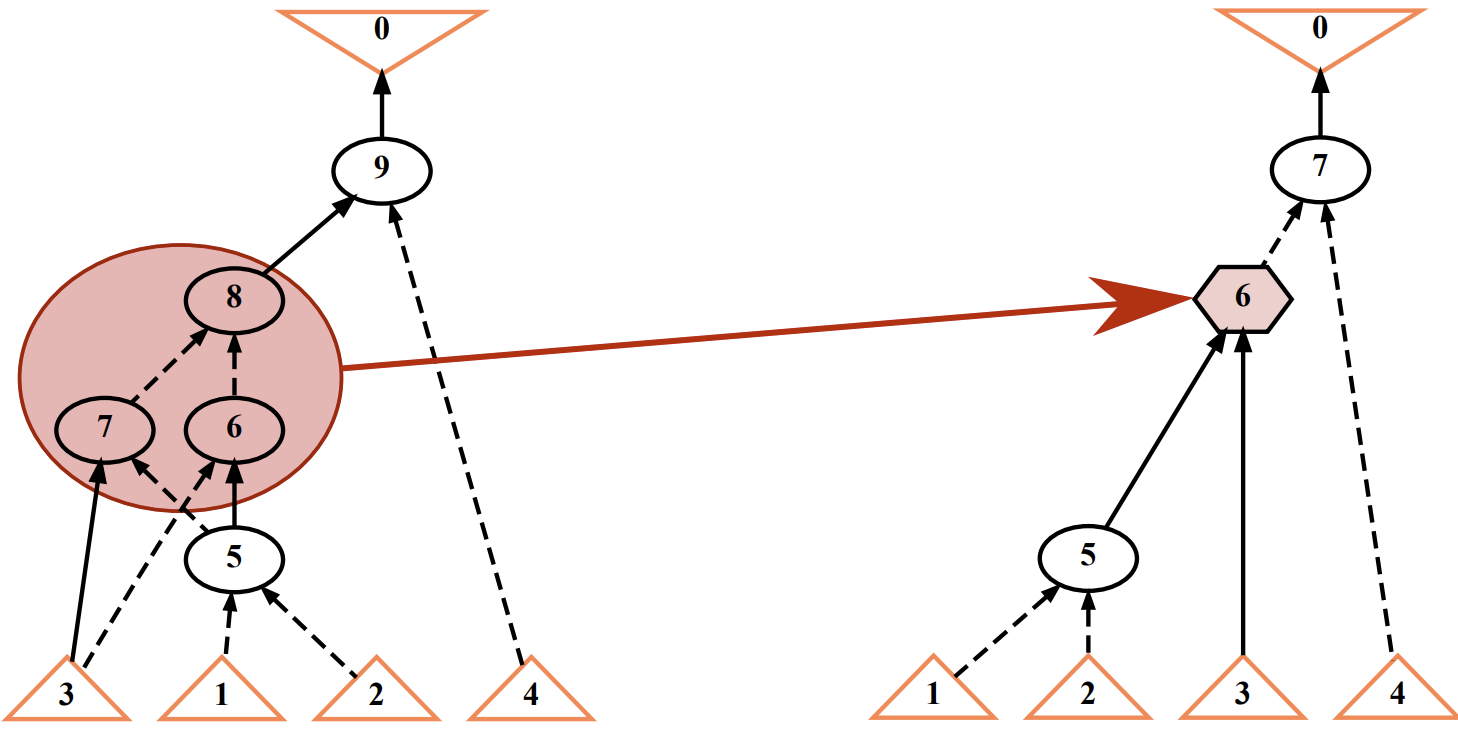
\includegraphics[width=0.75\linewidth]{./figs/LS-XAIG.png}
    \caption{函数$ \overline{ \overline{x_1 + x_2} \oplus x_3} \cdot \overline{x_4} $的AIG和XAIG,圆圈代表AND节点,六边形代表XOR节点,虚线边代表取反操作}
    \label{LS:XAIG}
\end{figure}

在AIG中,一个2输入异或门至少需要3个节点才能表示,这导致AIG无法对异或密集型电路进行高效地表示和优化,因此有工作提出了XAIG(Xor-And-Inverter Graph),在AIG中引入2输入的XOR节点,提高异或操作的表达效率\cite{LS:XAIG_Microelec_Relia,LS:XAIG_ddecs,LS:XAIG_iwls}。
图\ref{LS:XAIG}展示了函数$ \overline{ \overline{x_1 + x_2} \oplus x_3} \cdot \overline{x_4} $的AIG和XAIG,其中圆圈代表AND节点,六边形代表XOR节点,虚线边代表取反操作,可以看到XOR节点的引入能够降低图的规模。XAIG也被称为XAG(Xor-And Graph)。

(2)MIG

与XAIG的提出类似,有工作发现AIG能对控制电路进行高效地表达和变换,但对算术电路的操作效率较低,于是提出了适用于算术电路的MIG(Majority-Inverter Graph)\cite{LS:MIG}形式。在MIG中,除了输入节点外,每个节点表示一个3输入的Majority门,用符号$\langle \rangle$表示,定义为:
\begin{equation}
    \label{LS:MIG:Eq:Majority}
    \langle xyz \rangle = xy + xz + yz = (x + y) (x + z) (y + z)
\end{equation}

(3)XMG

对MIG引入3输入的XOR节点,能够提高某些函数的表达效率,对应的DAG实现被称为XMG(Xor-Majority Graph)\cite{LS:XMG_2017}。图\ref{LS:XMG}展示了函数$\langle x_1,x_2,(x_3 \oplus x_4) \rangle$分别在AIG、MIG和XMG中的表示,虚线代表取反操作,可以看到XMG使用的节点数目最少\cite{LS:XMG_2024}。

\begin{figure}[!htbp]
    \centering
    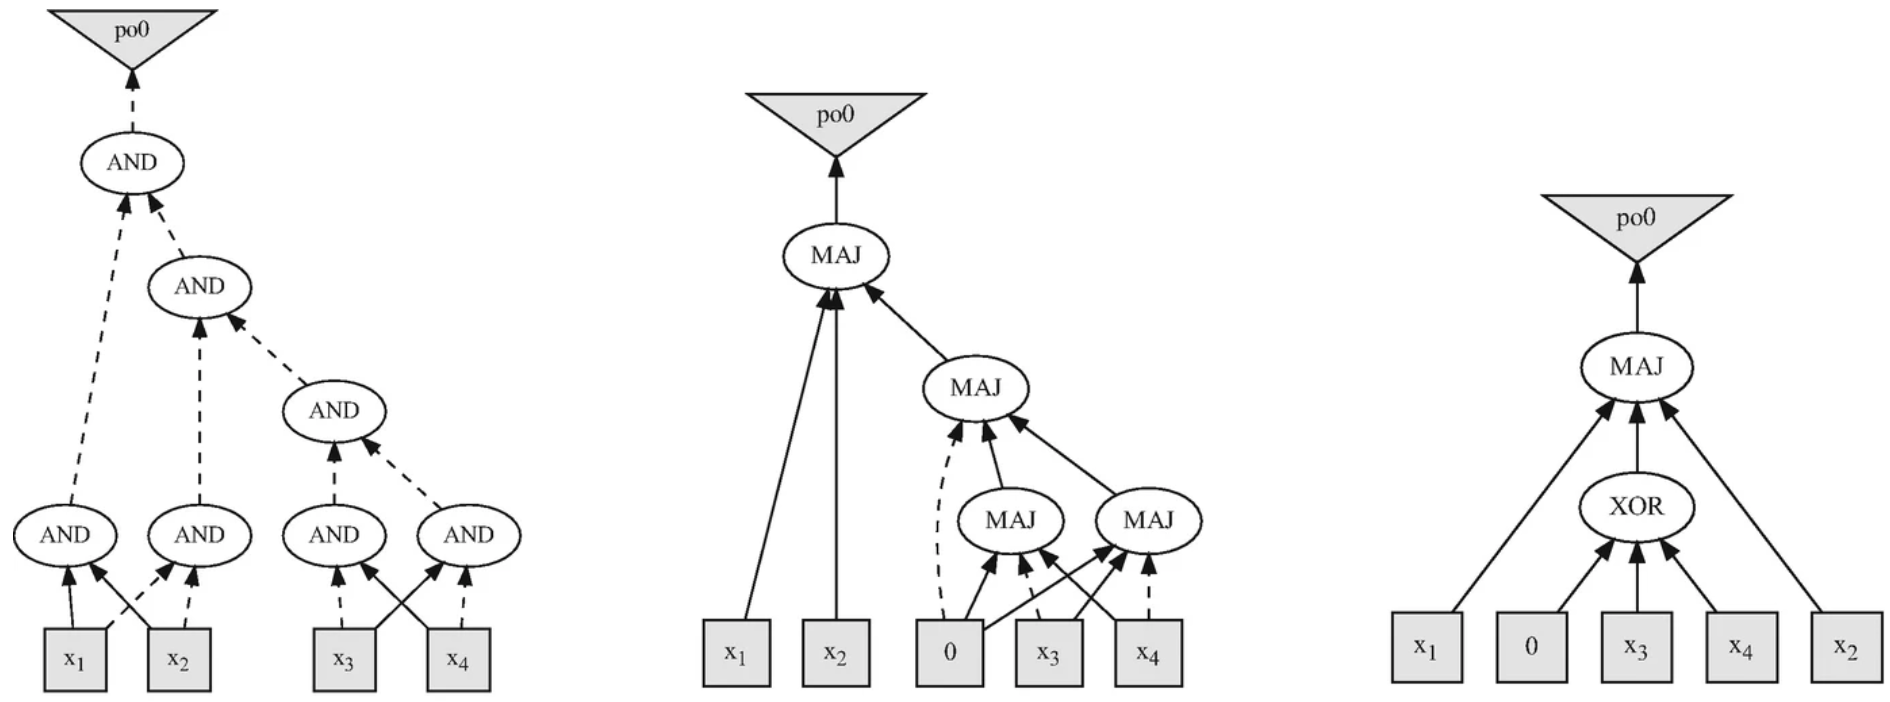
\includegraphics[width=\linewidth]{./figs/LS-XMG.png}
    \caption{函数$\langle x_1,x_2,(x_3 \oplus x_4) \rangle$分别在不同DAG中的表示,从左到右依次为:AIG、MIG、XMG,虚线代表取反操作}
    \label{LS:XMG}
\end{figure}

\subsection{MFFC} \label{MFFC}

在一个布尔网络中,节点$v$的一个锥(Cone)$C_v$是指$v$和$v$的传递扇入节点的集合(不包括网络的主要输入),锥中任意节点到$v$的路径都在锥内,$v$被称为锥的根节点,易知$v$可以有多个锥\cite{LS:exact_rewriting,FPGA:Jason_Cong_1993}。扇入节点数量小于等于$K$的锥被称为$K$可行锥($K$-feasible cone)\cite{FPGA:Jason_Cong_1999_cut_ranking}。

节点$v$在锥$C_v$下的一个割(Cut)是$C_v$的一个划分$(X,\overline{X})$,其中$\overline{X}$是$v$的一个锥。当$\overline{X}$是一个$K$可行锥时,割$(X,\overline{X})$被称为$K$可行割($K$-feasible cut)\cite{FPGA:Jason_Cong_1999_cut_ranking}。$\overline{X}$的扇入节点集合$L$满足以下两个性质:
\begin{itemize}
    \item 任意一条从网络的主要输入到节点$v$的路径至少会经过$L$中的一个元素;
    \item 对于$L$中的任何一个节点$l$,至少存在一条从主要输入到$v$的路径经过$l$且不经过$L$中的其他节点。
\end{itemize}
图\ref{LS:z_cone_two_cuts}展示了节点z的一个锥\{z,x,a,d,c,b,e\}和两个割\cite{FPGA:CLB_Anderson}cut1、cut2,易知cut1和cut2均是3可行割。
\begin{figure}[!htbp]
    \centering
    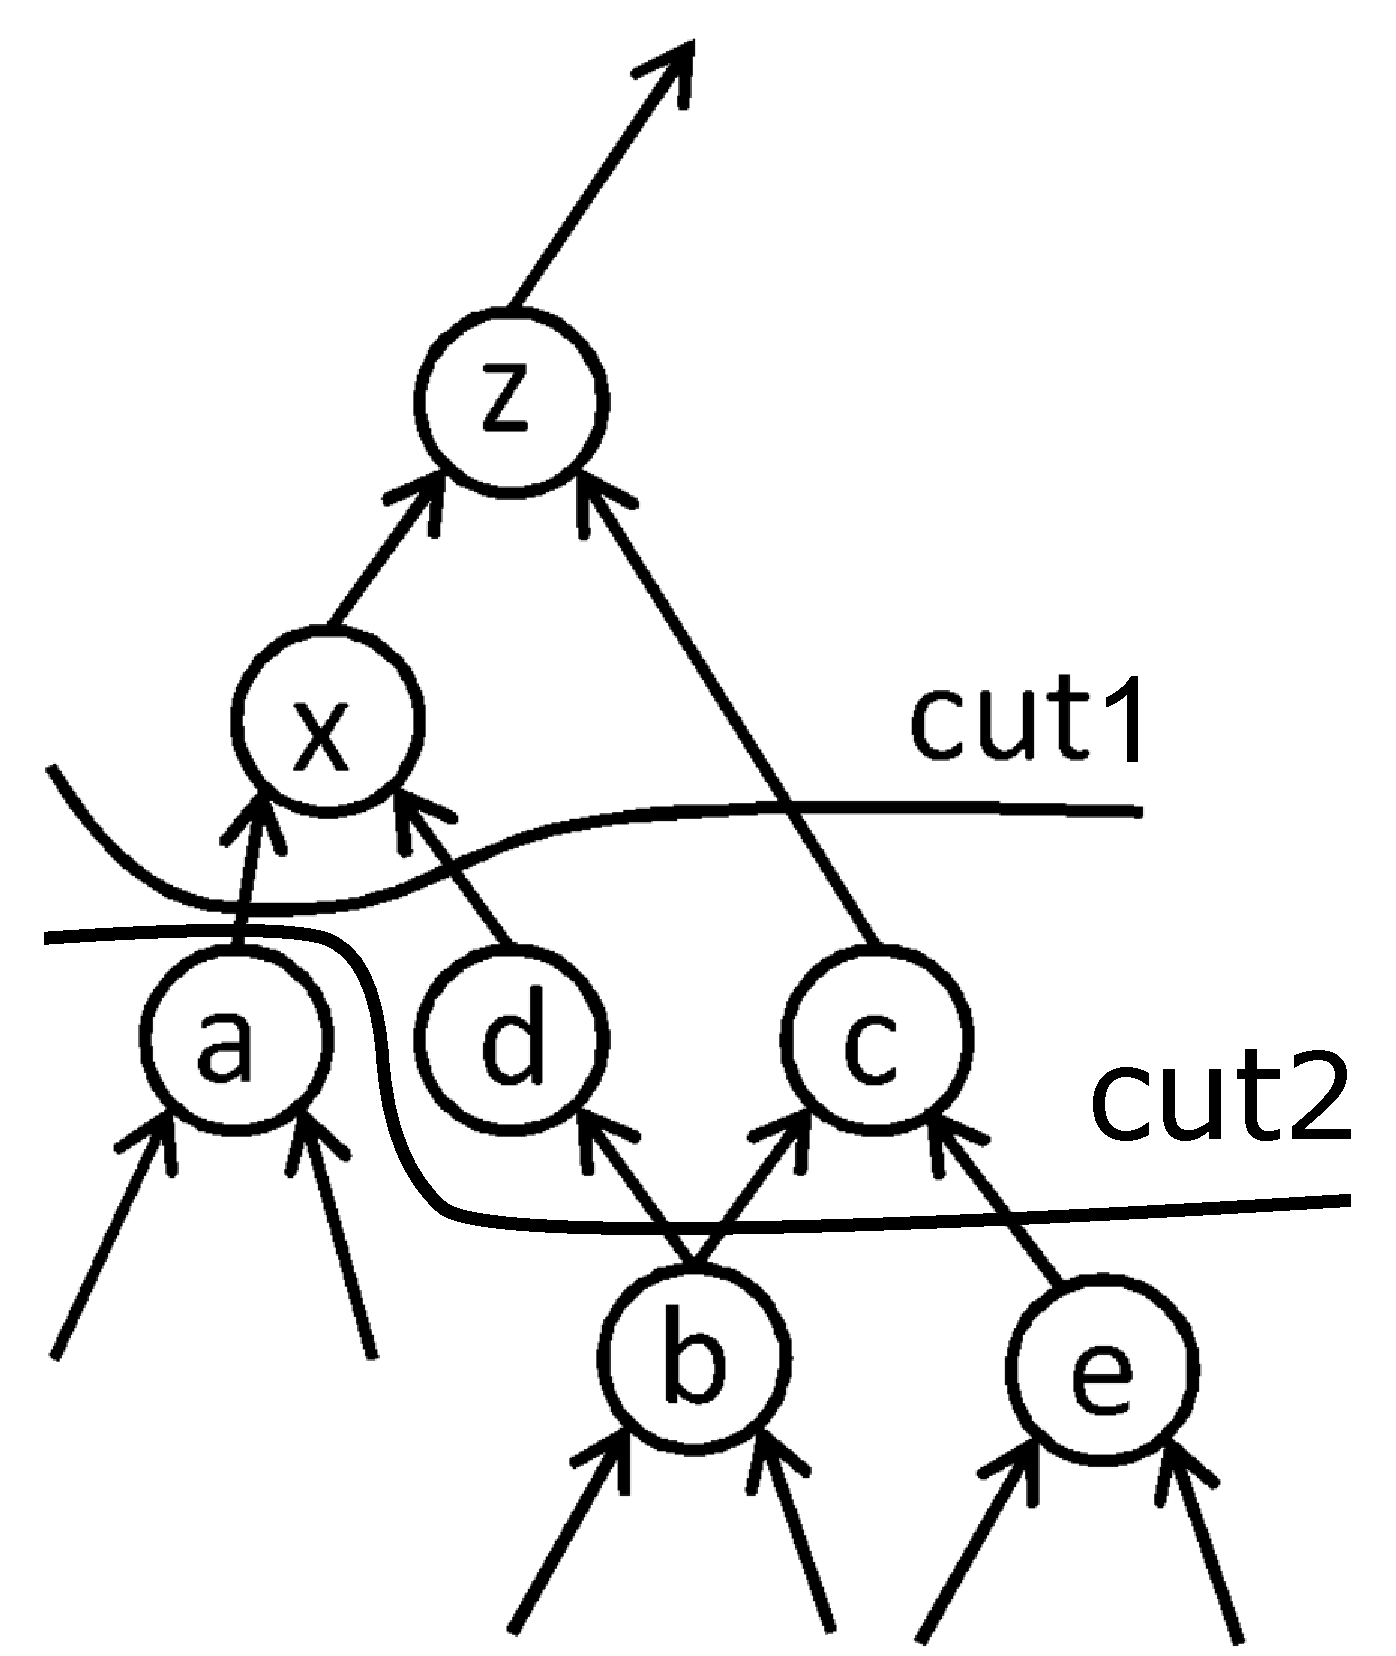
\includegraphics[width=0.4\linewidth]{./figs/LS-z_cone_two_cuts.pdf}
    \caption{节点z的一个锥\{z,x,a,d,c,b,e\}和两个割cut1与cut2}
    \label{LS:z_cone_two_cuts}
\end{figure}

若锥$C_v$内任意节点的扇出均在锥内,则称$C_v$为节点$v$的无扇出锥(Fanout Free Cone, FFC)。$v$的无扇出锥可以有多个,存在一个最大的无扇出锥,被称为$v$的最大无扇出锥(Maximum Fanout Free Cone, MFFC),记为MFFC$_v$。易知MFFC有以下性质\cite{LS:exact_rewriting,FPGA:Jason_Cong_1993,FPGA:Jason_Cong_patition}:
\begin{itemize}
    \item 一个节点的MFFC有且只有一个;
    \item 若 $w \in \text{MFFC}_v$,则$\text{MFFC}_w \subseteq \text{MFFC}_v$;
    \item 两个MFFC要么不相交,要么一个包含另一个;
    \item $\text{MFFC}_v$中节点的值只会影响到$v$和$v$的传递扇出。
\end{itemize}
\begin{figure}[!htbp]
    \centering
    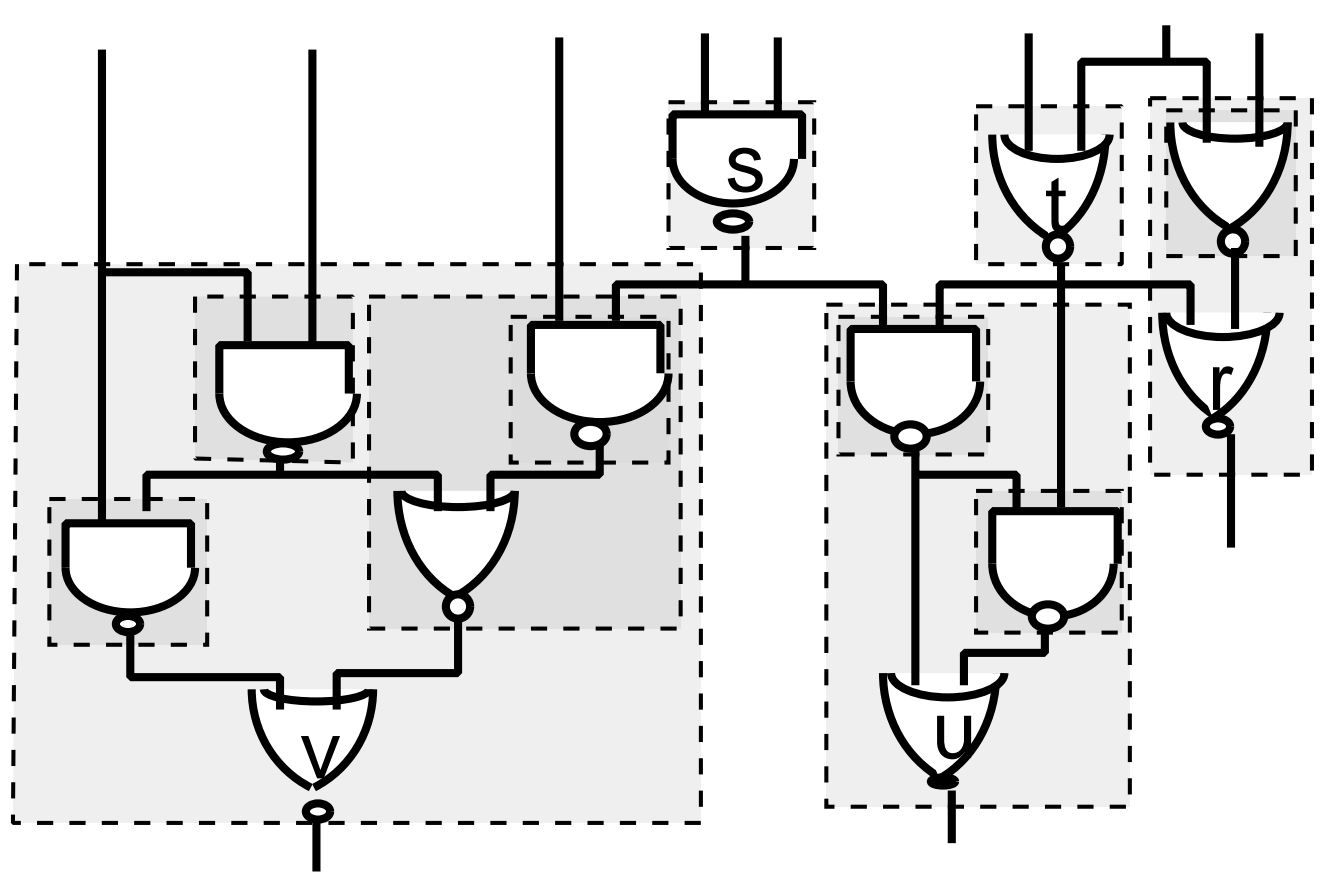
\includegraphics[width=0.5\linewidth]{./figs/LS-MFFC.png}
    \caption{不同节点的最大无扇出锥}
    \label{LS:MFFC}
\end{figure}
图\ref{LS:MFFC}展示了一个布尔网络中不同节点的MFFC,以不同灰度的阴影区域表示,可以看到各MFFC满足上述性质。


\subsection{电路划分}

当布尔网络的规模太大时,单个优化命令的运行时间变长,序列探索时单次迭代花费的时间显著增加,导致无法在一个可接受的时间范围内得到一个较优的命令组合,通过划分将大型网络分割成较小的子网络来并行地探索,能够大大减少运行时间。

(1)超图划分

一个网络的DAG图既可以转换成普通图(一条边只连接两个顶点),也可以转换成超图(一条边可以连接超过两个顶点),考虑到电路中的输出往往都是多扇出的,超图能够更好地体现其连接性,因此将电路转换成超图进行划分是一个较好的选择\cite{LS:LSOracle}。

\begin{figure}[!htbp]
    \centering
    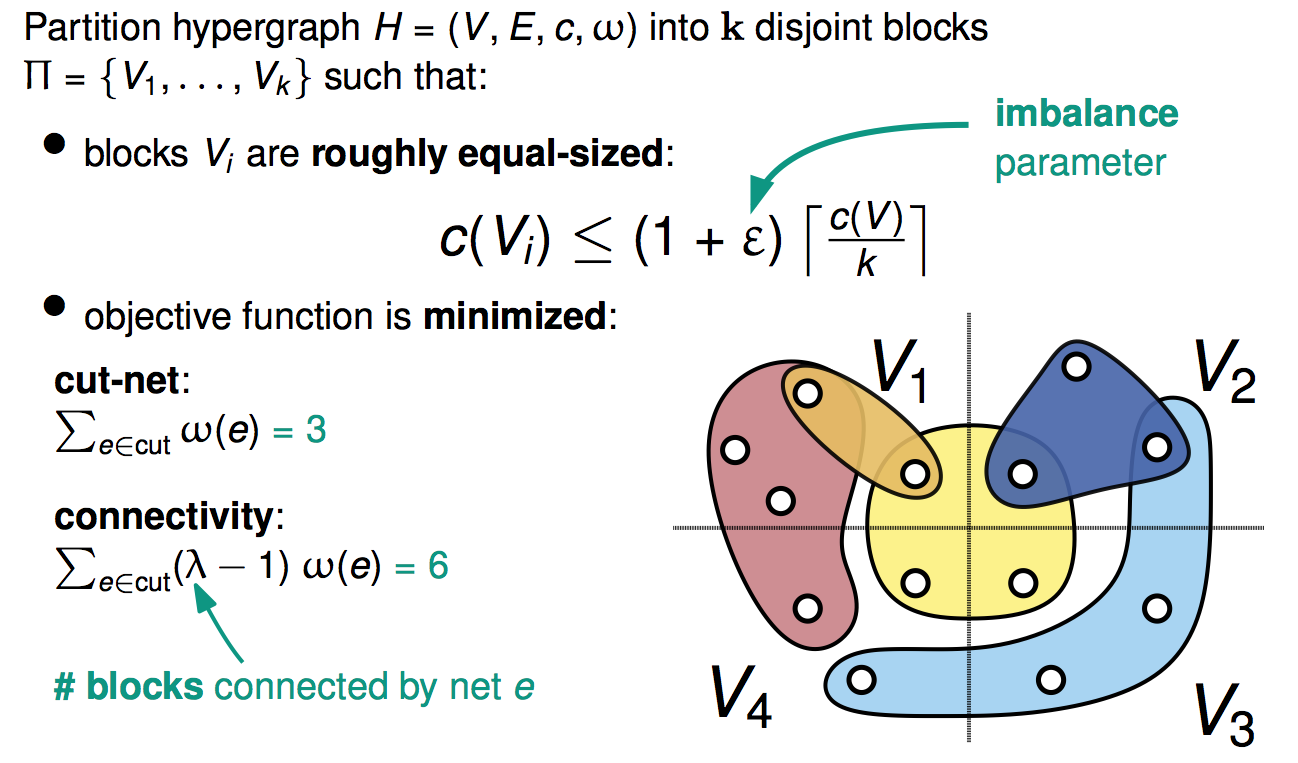
\includegraphics[width=0.8\linewidth]{./figs/Hypergraph_partition.png}
    \caption{超图划分问题的定义}
    \label{Hypergraph_partition}
\end{figure}

超图划分(Hypergrap partitioning)\cite{KaHyPar}能够对节点进行分类,将所有的节点划分为$k$个大致相等的部分,同时最小化基于边定义的目标函数,常见的目标函数有割边重要性和子图连通性,其中割边重要性是指被切割的超边的权重之和,而子图连通性则会同时考虑割边权重和割边连接的子图的数量。图\ref{Hypergraph_partition}展示了超图划分问题的定义以及两种目标函数的形式。
目前最常用的超图划分算法是多层(Multilevel)方法,由三个步骤组成:(1)粗化:对超图中不同连接紧密程度的点进行逐级合并以降低超图的规模;(2)初始划分:粗化完成后得到一个小的超图并对其进行初始划分;(3)细化:逐级分解原先合并的点并执行划分操作,每一次划分后利用局部搜索的方法来调整位于边界上的点以最小化目标函数,直到划分后子图的数目满足要求。

(2)自然划分

通常来讲,EDA工具对电路进行解析后生成布尔网络时会把寄存器与组合逻辑分开,将寄存器的输入变成组合逻辑的输出,将寄存器的输出变成组合逻辑的输入。有工作发现,良好设计的电路中流水线(Pipeline)技术充分,能够将整个电路“自然”地切分成数个均匀的组合逻辑块,转换成布尔网络后对应多个相互独立的DAG。基于此发现,文献\cite{Moucheng_Yang}提出了一种“自然划分(Natural partitioning)”的布尔网络分割方法,该方法基于ABC\cite{LS:ABC}实现,能够对一个大型AIG进行分簇,簇与簇之间没有连接,然后对所有的AIG簇并行地进行LUT映射以提高速度,对13个大型电路的测试结果表明,映射速度平均提高了5.76倍,面积略微增加了0.57\%,延迟保持不变。

(3)基于MFFC和带约束超图划分的有向无环划分

普通的超图划分并没有考虑DAG有向无环的特点,文献\cite{FPGA:Jason_Cong_patition}首先对一个网络进行遍历,利用MFFC缩小超图的规模,之后基于带约束的多层划分方法,提出了一个面向FPGA领域的有向无环划分方案,与普通超图划分相比割边数量更少、分割质量更高。

\subsection{强化学习}

强化学习是机器学习中的一个领域,强调一个智能体(Agent)如何基于环境(Environment)行动,以取得最大化的预期利益,是除了监督学习和非监督学习之外的第三种基本的机器学习方法。强化学习通过感知所处环境的状态(State)对动作(Action)的 反应(Reward),来指导更好的动作,从而获取最大的收益(Return)。以游戏为例,如果在游戏中采取某种策略可以取得较高的得分,那么就进一步“强化”这种策略,以期继续取得较好的结果。目前,强化学习在某些领域已经被证明了达到人类水平,甚至优于人类,比如早在2016年由谷歌研发的电脑围棋软件AlphaGo\cite{AI:AlphaGo}就已经击败了韩国围棋冠军李世石。

强化学习基于马尔科夫决策过程(Markov decision process),即当前状态包含了对未来预测所需要的所有信息,过去信息对未来预测不重要,关注点在于“探索未知领域”和“利用已有知识”的平衡,其实现算法分为有模型学习(Model-Based)和免模型学习(Model-Free)两类,其中免模型学习更容易实现,迁移性也更好,得到了广泛的研究。

\subsection{序列探索}

学术界提出了多种方法用来对逻辑综合中不同命令的组合及顺序进行探索,包括基于强化学习的方法、利用贝叶斯优化进行搜索、以及基于图神经网络进行预测等,下面分别进行介绍。

(1)基于强化学习的方法

\begin{figure}[!htbp]
    \centering
    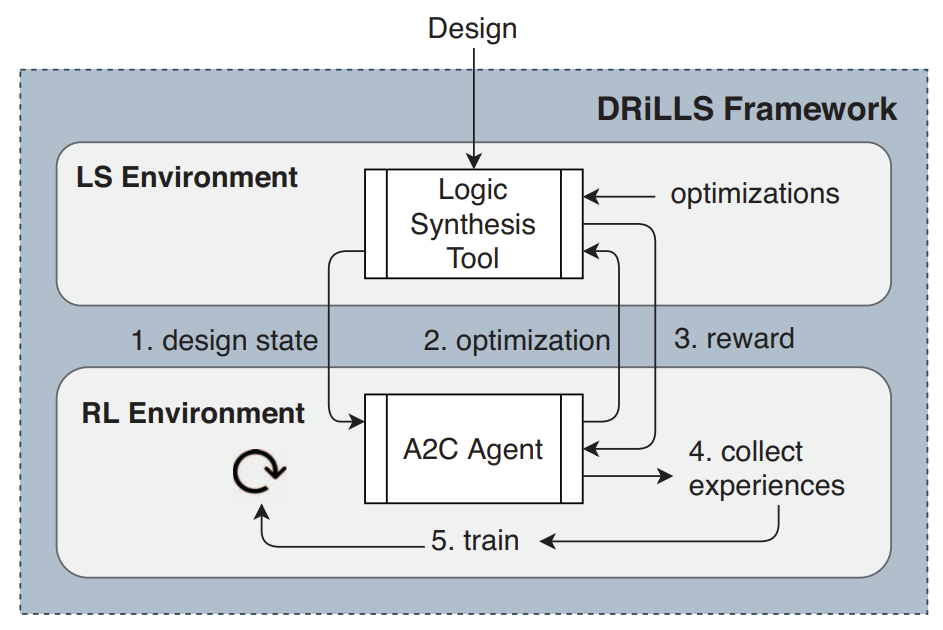
\includegraphics[width=0.7\linewidth]{./figs/LS-DRiLLS-framework.png}
    \caption{基于强化学习的序列优化方法DRiLLS的架构图}
    \label{LS:DRiLLS:Fig:framework}
\end{figure}

假设$\mathbb{A} = \{ a_1,\ a_2,\ a_3,\ \cdots,\ a_n \}$代表$n$个相互之间没有依赖的优化命令集合,$k$表示优化序列长度,则可能的命令组合情况一共有$n^k$种。
文献\cite{LS:DRiLLS}提出了一种基于强化学习的序列优化方法DRiLLS,DRiLLS利用A2C(Advantage Actor Critic)代理来探索序列空间。图\ref{LS:DRiLLS:Fig:framework}给出了DRiLLS的架构图,其中逻辑综合环境由Yosys和ABC实现,强化学习环境由A2C代理,与综合环境进行交互学习。DRiLLS将强化学习中的状态$state$定义为ABC中AIG的信息,包括主要输入输出数量、节点数、级数、寄存器数量、AIG中边的条数、以及AIG中反向边的数量。
同时,DRiLLS中强化学习的奖励函数是一个同时考虑面积和延迟的多目标函数,对于满足延迟约束且面积减少的优化序列,奖励最高(用+++表示),对于不满足延迟约束且面积增加的优化序列,奖励最低(用- - -表示),具体的奖励标准如表\ref{LS:DRiLLS:Table:reward}所示。

\begin{table*}[!htbp]
    \caption{DRiLLS中不同优化效果的序列对应的奖励情况}
    \centering
    \label{LS:DRiLLS:Table:reward}
    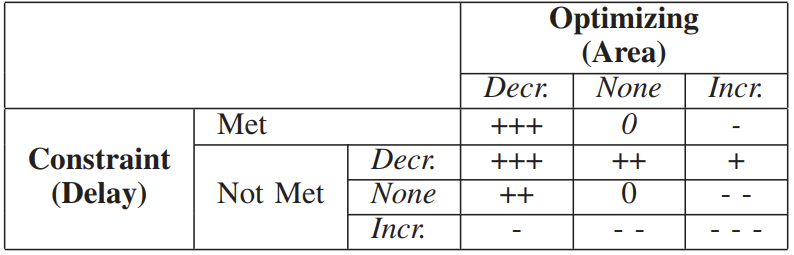
\includegraphics[width=0.7\linewidth]{./figs/LS-DRiLLS-reward_table.png}
\end{table*}

\begin{table*}[!htbp]
    \caption{实验结果}
    \centering
    \label{LS:DRiLLS:Table:results}
    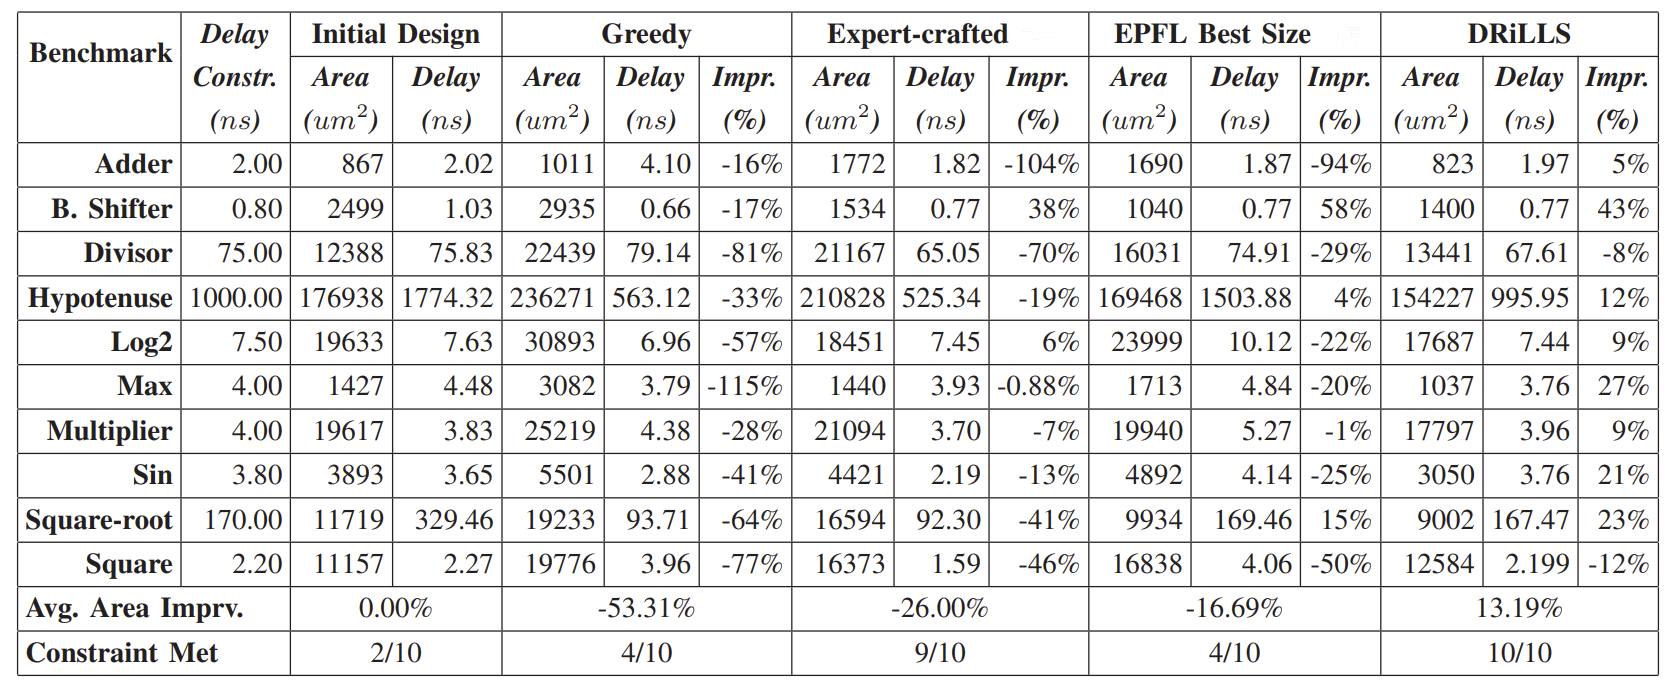
\includegraphics[width=\linewidth]{./figs/LS-DRiLLS-results.png}
\end{table*}

表\ref{LS:DRiLLS:Table:results}展示了基于ABC\cite{LS:ABC}和EPFL测试集\cite{LS:EPFL_benchs_iwls,LS:EPFL_benchs_github}通过4种方法包括贪婪算法(Greedy algorithm)、手工设计的优化序列\cite{LS:DRiLLS:hand_craft}(Expert-crafted)、已有的最佳记录、DRiLLS在开源的7nm工艺库\cite{ASAP7_github}上得到的实验结果,其中DRiLLS的延迟约束是初始的未优化的电路直接映射得到的延迟。
可以看到,DRiLLS在不同的电路上均满足了延迟约束,面积平均提高了13.19\%,这显示了DRiLLS多目标奖励函数的有效性。


(2)利用贝叶斯优化搜索

逻辑优化中的序列探索问题可以归结为黑盒优化问题,文献\cite{LS:BOiLS}提出了BOiLS,利用贝叶斯优化对命令的组合及顺序进行探索。基于ABC,对于一个给定的AIG,BOiLS的目标是在$n$个优化命令中找到一个长度为$K$的序列对电路进行优化,序列的好坏通过ABC进行LUT映射后来评估,其质量由下面的公式进行表达:
\begin{equation}
    \label{LS:BOiLS:Eq:QoR}
    QoR = \frac{Area(seq)}{Area(ref)} + \frac{Delay(seq)}{Delay(ref)}
\end{equation}
其中$Area(ref)$和$Delay(ref)$分别代表对原始电路用resyn2进行优化和映射后LUT的个数和级数,$Area(seq)$和$Delay(seq)$分别代表BOiLS找到的优化序列对原始电路进行优化和映射后LUT的个数和级数。在BOiLS中,考虑的优化命令包括:rewrite, rewrite -z, refactor, refactor -z, resub, resub -z, balance, fraig, sopb, blut, dsdb,序列大小$K=20$。

\begin{figure}[!htbp]
    \centering
    \includegraphics[width=\linewidth]{./figs/LS-BOiLS-results.png}
    \caption{不同序列探索方法在迭代200次后的LUT映射结果}
    \label{LS:BOiLS:Fig:results}
\end{figure}

\begin{figure}[!htbp]
    \centering
    \includegraphics[width=\linewidth]{./figs/LS-BOiLS-results_2.png}
    \caption{不同方法在4个电路上的探索效率对比}
    \label{LS:BOiLS:Fig:results_2}
\end{figure}

基于EPFL电路集\cite{LS:EPFL_benchs_iwls,LS:EPFL_benchs_github},BOiLS与6个前沿工作进行了对比,包括:基于强化学习方法的DRiLLS\cite{LS:DRiLLS},标准贝叶斯优化(Standard Bayesian Optimization, SBO),遗传算法(Genetic Algorithm, GA),随机搜索(Random Search, RS),以及已有的最佳记录。每种方法限制的迭代次数为200,图\ref{LS:BOiLS:Fig:results}展示了不同方法的实验结果。可以看到,BOiLS在8/10个电路中都取得了最优结果,SBO在log2电路中效果最好,BOiLS紧随其后,显示了贝叶斯优化在逻辑综合序列探索中的巨大潜力。图\ref{LS:BOiLS:Fig:results_2}比较了不同优化方法在4个电路上的探索效率,结果显示,基于强化学习的序列搜索方法DRiLLS看起来似乎并没有比随机搜索强多少。

(3)基于图神经网络的方法

图卷积网络(Graph Convolutional Network, GCN)是一种用于处理图数据的深度学习模型,其目标是将传统的卷积神经网络和递归神经网络等深度学习方法扩展到图结构数据如社交网络、推荐系统、生物信息学等领域,填补深度学习对图数据处理方式的空缺。

\begin{figure}[!htbp]
    \centering
    \includegraphics[width=0.7\linewidth]{./figs/LS-Bulls-Eye-QoR_predictor.png}
    \caption{基于AIG和GCN的序列质量预测器}
    \label{LS:Bulls-Eye:Fig:QoR_predictor}
\end{figure}

\begin{figure}[!htbp]
    \centering
    \includegraphics[width=0.9\linewidth]{./figs/LS-Bulls-Eye-overall_framework.png}
    \caption{Bulls-Eye整体框架图}
    \label{LS:Bulls-Eye:Fig:overall_framework}
\end{figure}

文献\cite{LS:Bulls-Eye}首先利用GCN基于AIG提出了一个序列质量预测器,总体结构如图\ref{LS:Bulls-Eye:Fig:QoR_predictor}所示。预测器的输入包括AIG和优化命令序列(图中的Synthesis recipe),两者分别通过AIG嵌入网络和序列嵌入网络进行嵌入,拼接后经过四层全连接层进行输出。之后,在基于小型电路集上对预测器进行训练后,面对新的大型电路,通过主动学习(Active learning)的方式对预测器进行微调,以提高对新电路的预测准确率。最后,基于微调后的预测器,利用模拟退火算法对新电路生成一个高质量的优化序列,整体框架命名为Bulls-Eye,流程如图\ref{LS:Bulls-Eye:Fig:overall_framework}所示。Bulls-Eye的预测器在基于44个开源电路设计组成的数据集上进行训练,实验表明,训练后的模型在新的大型电路的序列质量预测任务中表现良好,微调后的模型准确率进一步上升。

\subsection{多种DAG联合优化}

基于MIG对算术电路的综合及映射效果比AIG更好这一特点,文献\cite{LS:LSOracle}提出了LSOracle,是第一个同时采用多种DAG形式对布尔逻辑电路进行表示和优化的开源异构逻辑综合框架。

\begin{figure}[!htbp]
    \centering
    \includegraphics[width=0.7\linewidth]{./figs/LS-LSOracle-flow.png}
    \caption{LSOracle流程图}
    \label{LS:LSOracle:Fig:flow}
\end{figure}

图\ref{LS:LSOracle:Fig:flow}展示了LSOracle的工作流程图,输入电路首先被转换成AIG,然后变成超图。
接着利用开源的超图划分工具KaHyPar\cite{KaHyPar}将其分割成多个子图,子图之前存在松散的连接。
之后,分类引擎会利用二维图片对子图进行表示,并利用神经网络对图片进行分类,对每个子图挑选出一种最适合的DAG表示(AIG或MIG)并优化。具体来讲,设$B=\{0,\ 1\}$,一个$n$输入的布尔函数是一个从$B^n$到$B$的映射:$f: B^n \rightarrow B$。因此,一个$n$输入的布尔函数可以由一个$n$维空间表示,卡诺图是一种利用二维空间完成$n$维空间映射的表示形式。受卡诺图启发,LSOracle提出了一种用二维图片来表示逻辑函数的方法,命名为KMImage(Karnaugh-Map Image)。
\begin{figure}[!htbp]
    \centering
    \includegraphics[width=0.9\linewidth]{./figs/LS-LSOracle-KMImage.png}
    \caption{将卡诺图转变为KMImage的示例}
    \label{LS:LSOracle:Fig:KMImage}
\end{figure}
图\ref{LS:LSOracle:Fig:KMImage}展示了一个将卡诺图转换为KMImage的例子,在KMImage中,每个像素点对应卡诺图中的一个输出,卡诺图中数值为1的输出在KMImage中以灰色像素表示,卡诺图中数值为0的输出在KMImage中以黑色像素表示。这种表示方法类似于MNIST\cite{DNN:LeNet_MNIST}数据集中的图片表示方法。在MNIST中,每张图片包含28×28个像素点,由黑白两种颜色组成。
通过将布尔函数转换为二维图片,能够利用计算机视觉领域成熟的研究方法对KMImage的特征进行识别和分类,挑选出最适合对应真值表实现的DAG格式。
一个$N \times N$大小的KMImage可以表示任意一个输入数为$2log_2 N$的逻辑函数,易知同一逻辑函数在改变输入顺序后对应不同的KMImage(除非函数是对称的),有可能导致分类结果不一致。然而,一个逻辑函数只会对应一种最优的DAG实现,分类错误会导致电路性能的下降,LSOracle并没有考虑改变输入顺序后有可能得到更优DAG分类的情况,这是其考虑不周的地方。

超图划分后的子图往往是多输出函数,KMImage只能表示单输出函数,为了解决多输出函数子图的分类问题,LSOracle采用了一种计分机制。具体来讲,分类引擎根据所有主要输出节点的最大逻辑锥(见\ref{MFFC}有关锥的定义)得到多个KMImage并赋予不同的权重,节点数目越多、网络深度越大的锥的权重越大。在对每个KMImage进行分类之后,分别计算不同DAG的总得分,得分最高的DAG作为该子图的最终分类结果,计算公式如下所示:
\begin{equation}
\label{LS:LSOracle:Eq:score}
score = \sum_{i=1}^{m} ( W_{ni} * N_i +W_{di} *D_i )
\end{equation}
式中$m$是子图的主要输出数,也是KMImage的个数;$N_i$和$W_{ni}$分别是第$i$个KMImage对应的锥的节点数和节点数权重;$D_i$和$W_{di}$分别是第$i$个KMImage对应的锥的深度和深度权重。LSOracle的分类器采用大小为$256 \times 256$的固定尺寸的KMImage,可以表示不超过16个输入的逻辑函数。对于小于16个输入的逻辑函数,通过随机填充的方法将KMImage扩展到$256 \times 256$大小。对于超过16个输入的逻辑函数,直接通过启发式算法对其进行分类:如果一个锥的逻辑深度超过所在子图逻辑深度的40\%,那么该锥被分类到MIG,否则被分类到AIG,所有锥分类完成后根据式\eqref{LS:LSOracle:Eq:score}计算不同DAG的得分,最终得到该子图的分类结果。一旦一个子图分类完成,该子图立刻被转化成对应的DAG格式,由预先指定的优化脚本进行优化,当所有的子图优化完成后,合并优化后的子图并将整个电路转换成MIG,进行最后的优化并输出。

LSOracle的分类算法具有一定的局限性:(1)KMImage具有固定尺寸,只能表示不大于16个输入数的逻辑函数,对小于16个输入数的布尔函数采用“随机补全”的办法,存在不确定性,影响分类精度;(2)划分后的子图往往是多输出的,然而KMImage只能表示单输出函数,即使能够利用多个KMImage对子图进行表征,但多个KMImage对应的布尔网络(锥)之间存在重复的节点,带来了重复的计算,影响分类精度。解决这两个问题可以采用基于图神经网络(Graph Neural Network, GNN)对子图进行分类的方法,GNN不受电路规模和输出个数的影响,能够极大地提高分类效率。



\section{本章小结}

本章首先介绍了精确定点数乘法器的三个运算过程:部分积的生成、累加、最终相加,以及每个过程不同的硬件实现方法。其中,
% 无符号数相乘的部分积可由与门直接产生,
补码有符号数乘法的部分积
% 根据设计方法的不同有多种生成方式,目前
最常用的生成方法是改进的Baugh-Wooley算法和基4的布斯算法。对于部分积的累加,通过将全加器排列为树形,采用进位保存的思想可得到较为高速的累加阵列。累加结束后
% 部分积的数量减少为2个,
需要一个多位宽的向量加法器完成最终相加,可根据需要采取不同结构。
% 可选择行波进位加法器、超前进位加法器、进位选择加法器、并行前缀加法器等不同结构。
接着介绍了由Mitchell发明的对数乘法器,该乘法器可将乘法转变为加法,大大降低了运算量,误差最大不超过$\dfrac{1}{9}$。
本章之后介绍了用来衡量近似电路误差的不同指标,这些指标均适用于近似乘法器。
最后介绍了已有的ASIC近似乘法器和FPGA近似乘法器设计方法以及逻辑综合相关技术。其中,ASIC近似乘法器设计方法可分为手工设计、数学转换近似、自动化方法和近似电路综合四类,FPGA近似乘法器大部分采用手工修改LUT编码的方式实现。这些工作不仅缺乏对数据分布和输入极性的考虑,同时存在效率低、灵活性差等缺点。对逻辑综合来讲,已有的工作着重在传统逻辑综合的优化序列探索上,如何结合近似单元库对大电路进行高质量的近似实现是一个需要考虑的问题。